\documentclass{article}
\usepackage[utf8]{inputenc}
\usepackage{graphicx}
\usepackage{amsmath}
\usepackage[margin=1.0in]{geometry}
\usepackage{float}
\usepackage{hyperref}
\usepackage{subcaption}
\usepackage{listings}
\usepackage{color}
\usepackage{enumerate}
\usepackage{enumitem}
\usepackage{caption}
\usepackage{hhline}
\usepackage{tabularx}



\title{Predicting COMPASS/AMBER Acceptance with Neural Networks}
\author{Pedro M. P. Curvo \\ Supervisor: Marcin Stolarski}
\date{\today}

\begin{document}
\maketitle

\begin{abstract}
    The COMPASS experiment, conducted at CERN (the European Organization for Nuclear Research),
    is a global effort to explore the subatomic world, delving into the intricate structure and properties of hadrons.
    This paper focuses on the prediction of particle's acceptance by a Neural Network, since the GEANT4 simulation
    is very time consuming. The data used for the analysis was generated using a LEPTO generator and the full
    simulation of the COMPASS spectrometer was done using the GEANT4 programme. 
    The neural network architecture and training process involved two models with different depths and activations.
    Chi-squared tests are used to evaluate model performance. While accuracy and loss metrics are monitored during
    training, chi-squared values are the key evaluation criteria. Multiple training iterations are conducted to
    account for chi-squared instability, with the best models selected post-training.
    Furthermore, the models are evaluated on a separate dataset to gauge their generalization capabilities.
    We also explore the possibility of reconstructing the spectrometer's structure using muon and hadron angles.
    Despite the challenges presented by this complex problem, the models show promise in predicting the acceptance
    of COMPASS/AMBER. Future work could explore alternative neural network architectures to further improve the
    models.

\end{abstract}

\section{Introduction}

\subsection{COMPASS/AMBER}

The COMPASS experiment, short for "Common Muon and Proton Apparatus for Structure 
and Spectroscopy," is a cutting-edge particle physics experiment conducted at CERN, 
the European Organization for Nuclear Research, in Geneva, Switzerland. COMPASS is a 
collaborative endeavor involving scientists and researchers from institutions around the world.
This experiment is dedicated to unraveling the mysteries of the subatomic world by probing the 
structure and properties of hadrons, which are particles composed of fundamental constituents 
called quarks and held together by the strong nuclear force. COMPASS achieves this by utilizing 
a high-energy polarized muon beam, making it unique in its precision measurements of hadron 
physics and spin properties.
With its sophisticated array of detectors, including spectrometers and tracking chambers, 
COMPASS captures and analyzes particles produced during high-energy collisions, providing 
valuable insights into the internal structure of nucleons like protons and neutrons. 
Additionally, COMPASS explores the production of exotic hadrons, expanding our understanding 
of the strong force interactions and the fundamental constituents of matter.
The data generated by the COMPASS experiment contributes significantly to advancing our 
knowledge of the building blocks of the universe and the forces that govern them, 
furthering our understanding of the intricacies of particle physics.


\section{Data Origin and Preprocessing}

\subsection{Data Origin: Generation and Reconstruction}
The data used for the analysis presented in this paper was generated using a LEPTO generator,
a dedicated generator for deep inelastic scattering (DIS) processes. Beyond that, the full simulation
of the COMPASS spectrometer was done using the GEANT4 programme. The data was then reconstructed
using the COMPASS reconstruction software. With this process, two files were generated for each type of events (Hadrons and Inclusive), one with the
Monte Carlo (MC) data, and another with the reconstructed data. 
The goal with this data is to check if it is possible to predict the acceptance of the COMPASS/AMBER
using a Neural Network, since the GEANT4 simulation is very time consuming, aproximately 30 seconds per event.
That might not seem like a lot, but when you have millions of events, it becomes a problem.
Therefore, one could use a Neural Network to have a better idea of how changed parameters affect the data/MC
agreement, and then only run the GEANT4 simulation for the events that are more likely to be accepted.


\subsection{Data Variables}
In this study, we used two types of events, Inclusive and Hadrons. The Inclusive events are events where the muon is detected, while the Hadrons events are events where hadrons are detected.
The data used for the analysis of the Inclusive events has 11 variables:

\begin{table}[H]
    \centering
    \begin{tabular}{c|l}
    \textbf{Variable} & \textbf{Description} \\ \hline
    $X_b$ & $Bjorken_x$ \\
    $Y$ & Virtual Photon Energy Fraction of the initial momentum\\
    $Q^2$ & Four-momentum transfer \\
    $Trig$ & Trigger \\
    $PV_z$ & X-Position of interaction vertex in the target\\
    $PV_x$ & Y-Position of interaction vertex in the target\\
    $PV_y$ & Z-Position of interaction vertex in the target\\
    $Mom_{mu}$ & Incoming beam momentum\\
    $Mom_{mup}$ & Outgoing muon momentum\\
    $d_xd_zmup$ & Angle of Muon \\
    $d_{y}d_{z}mup$ & Angle of Muon \\
    \end{tabular}
\end{table}

While the data used for the analysis of the Hadrons events has 16 variables:

\begin{table}[H]
    \centering
    \begin{tabular}{c|l}
    \textbf{Variable} & \textbf{Description} \\ \hline
    $X_b$ & $Bjorken_x$ \\
    $Y$ & Virtual Photon Energy Fraction of the initial momentum\\
    $Z$ & Fraction of hadron energy to the virtual photon energy \\
    $Q^2$ & Four-momentum transfer \\
    $Trig$ & Trigger \\
    $PV_z$ & X-Position of interaction vertex in the target\\
    $PV_x$ & Y-Position of interaction vertex in the target\\
    $PV_y$ & Z-Position of interaction vertex in the target\\
    $Mom_{mu}$ & Incoming beam momentum\\
    $Mom_{mup}$ & Outgoing muon momentum\\
    $d_xd_zmup$ & Angle of Muon \\
    $d_yd_zmup$ & Angle of Muon \\
    $q$ & Hadron Charge \\
    $mom$ & Momentum of Hadron \\
    $d_xd_z$ & Angle of Hadron \\
    $d_yd_z$ & Angle of Hadron \\
    \end{tabular}
\end{table}



As mentioned before, for each type of events, we have a file with the Monte Carlo data and another with the reconstructed data.
Since the goal is to find a way to predict the acceptance of the COMPASS/AMBER, we created a new variable, called "Accepted",
which is 1 if the event was accepted and 0 if it was rejected. Therefore, for the data with the Monte Carlo information, we added
a column with the value 1 for all the events, and for the data with the reconstructed information, we added a column with the value 0.
It's important to refer that the number of events for each of the files is different, since the Monte Carlo data has more events than the reconstructed data.
Hence, we had to balance the data for the training and testing of the Neural Network, which will be explained in the following sections.

\subsection{Data Visualization}
In order to have a better understanding of the data, we plotted the histograms for each of the variables, for the Inclusive and Hadrons events.

\textbf{The histograms for the Inclusive events are shown in the figures below:}

\begin{figure}[H]
    \centering
    \begin{subfigure}[b]{0.45\textwidth}
        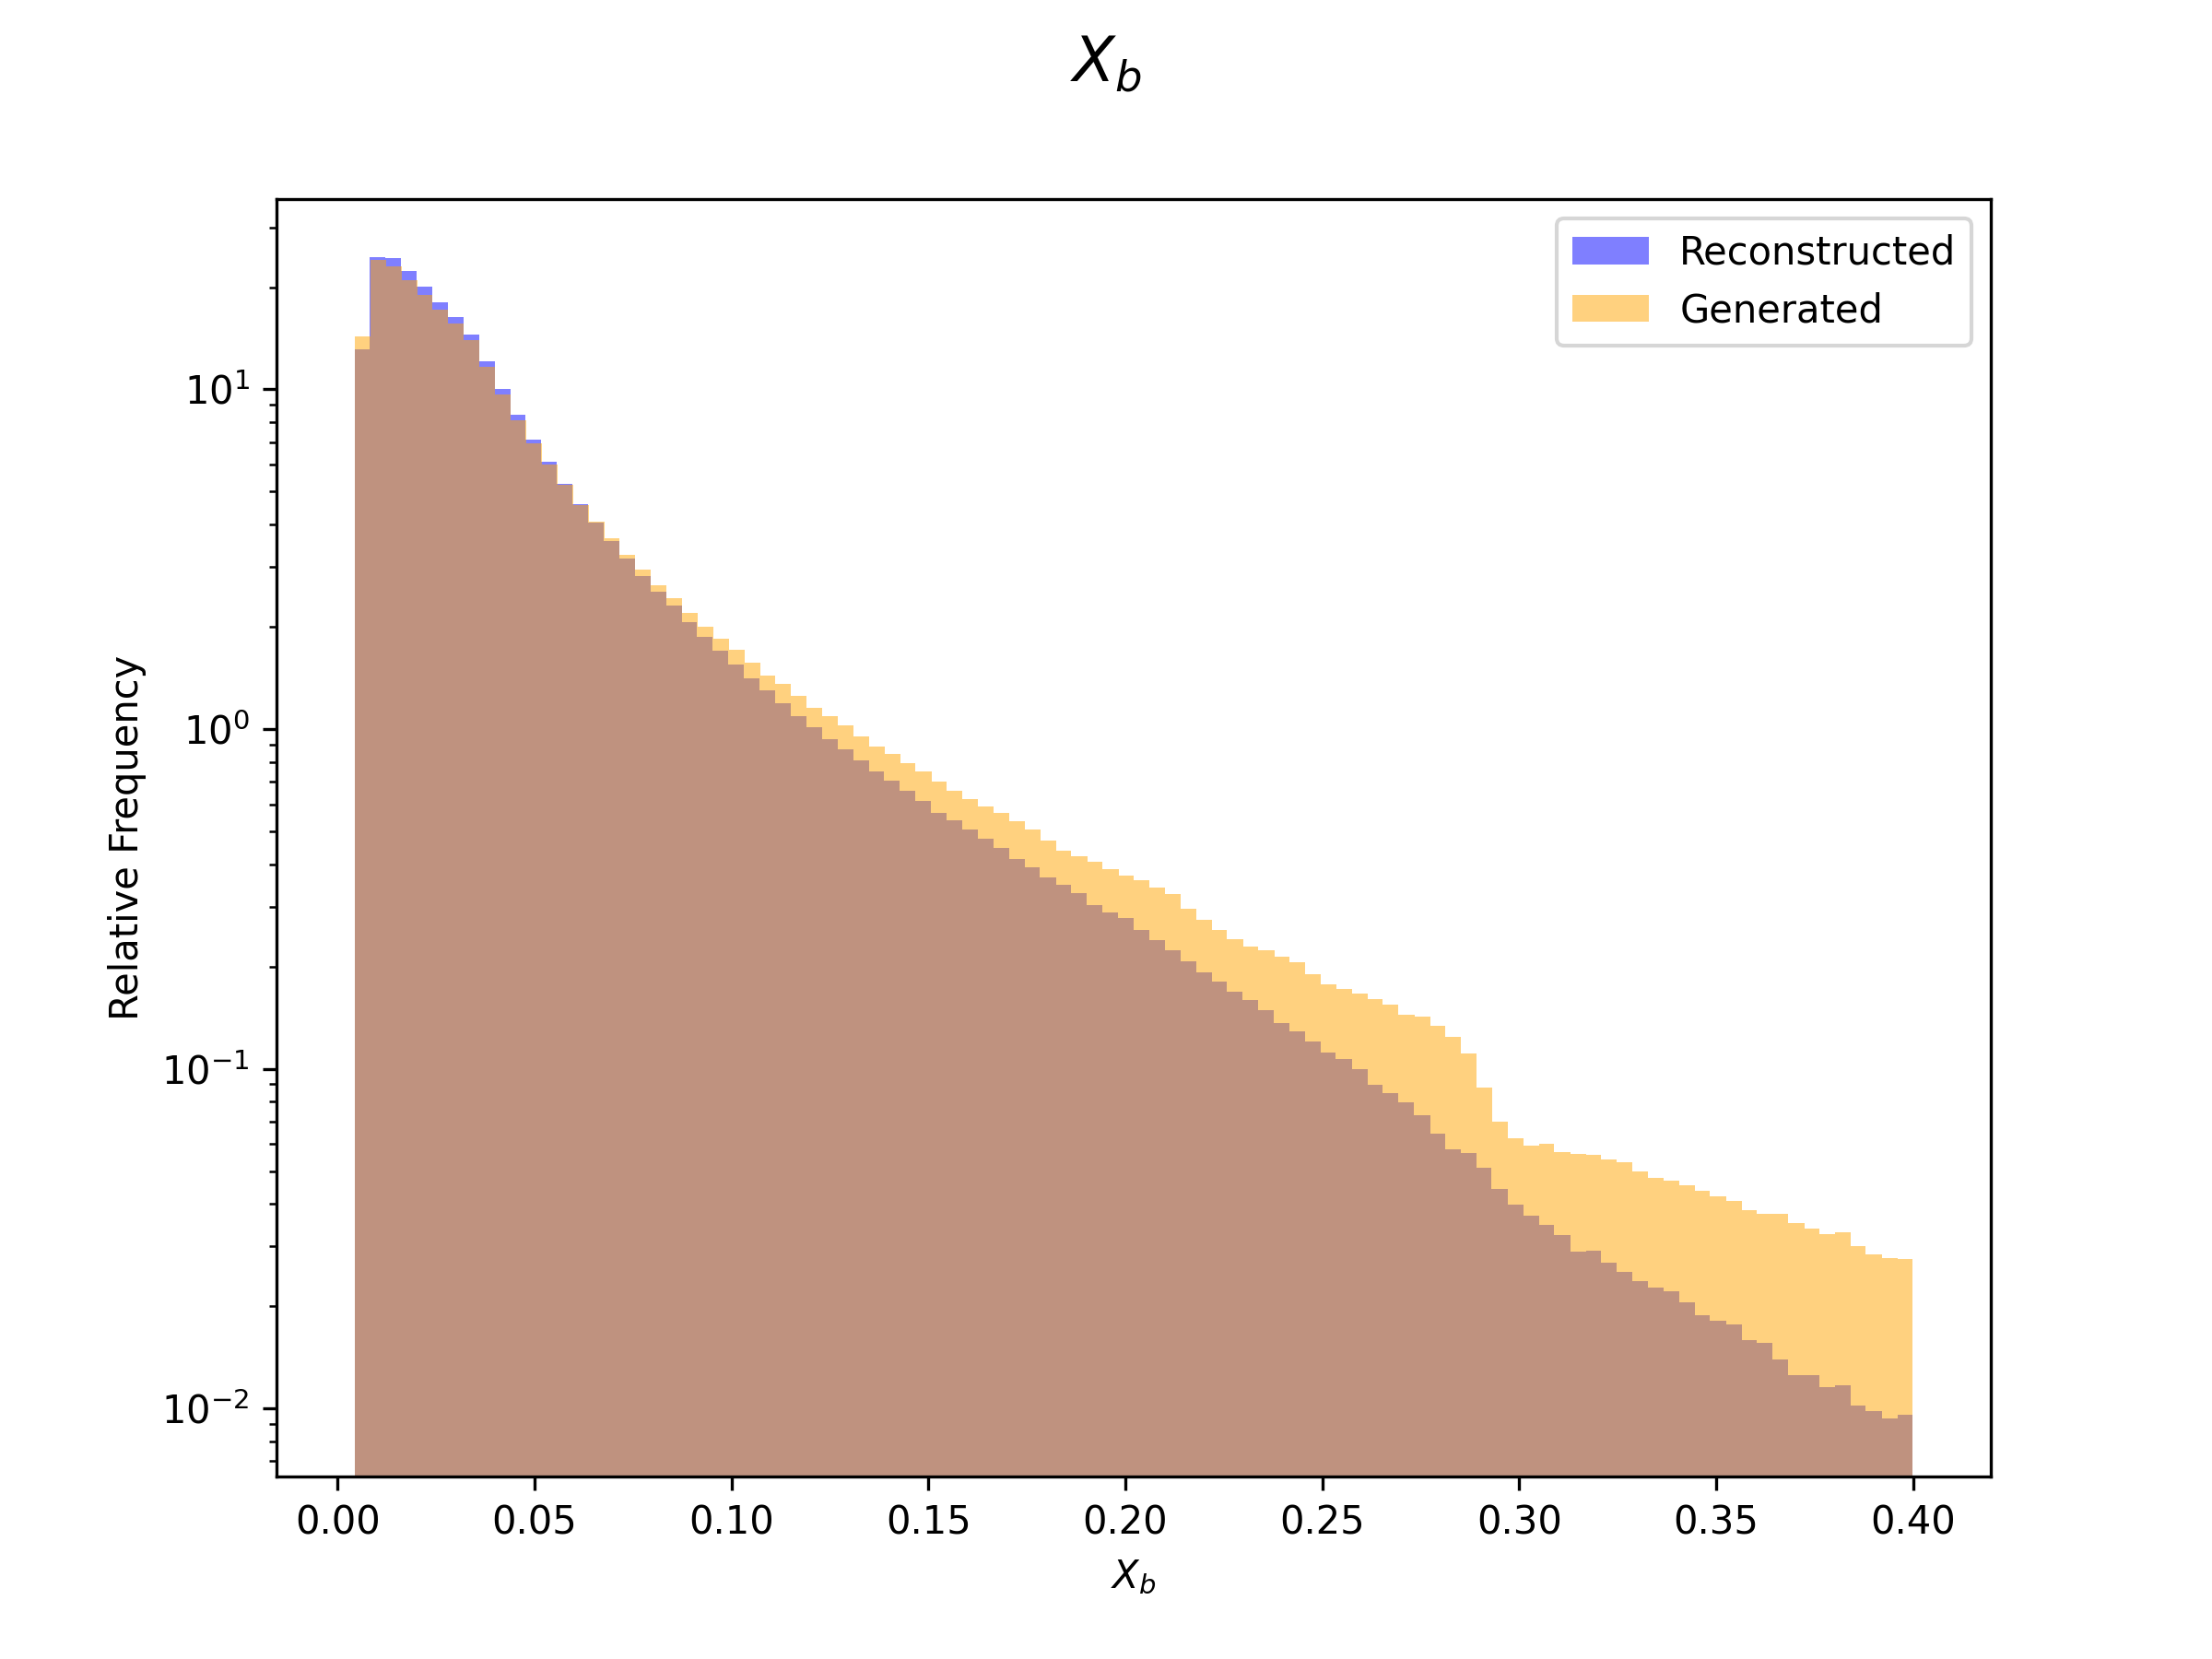
\includegraphics[width=\textwidth]{graphs/incl_X_b.png}
        \caption{Histogram for $X_b$}
        \label{fig:incl_X_b}
    \end{subfigure}
    \hfill
    \begin{subfigure}[b]{0.45\textwidth}
        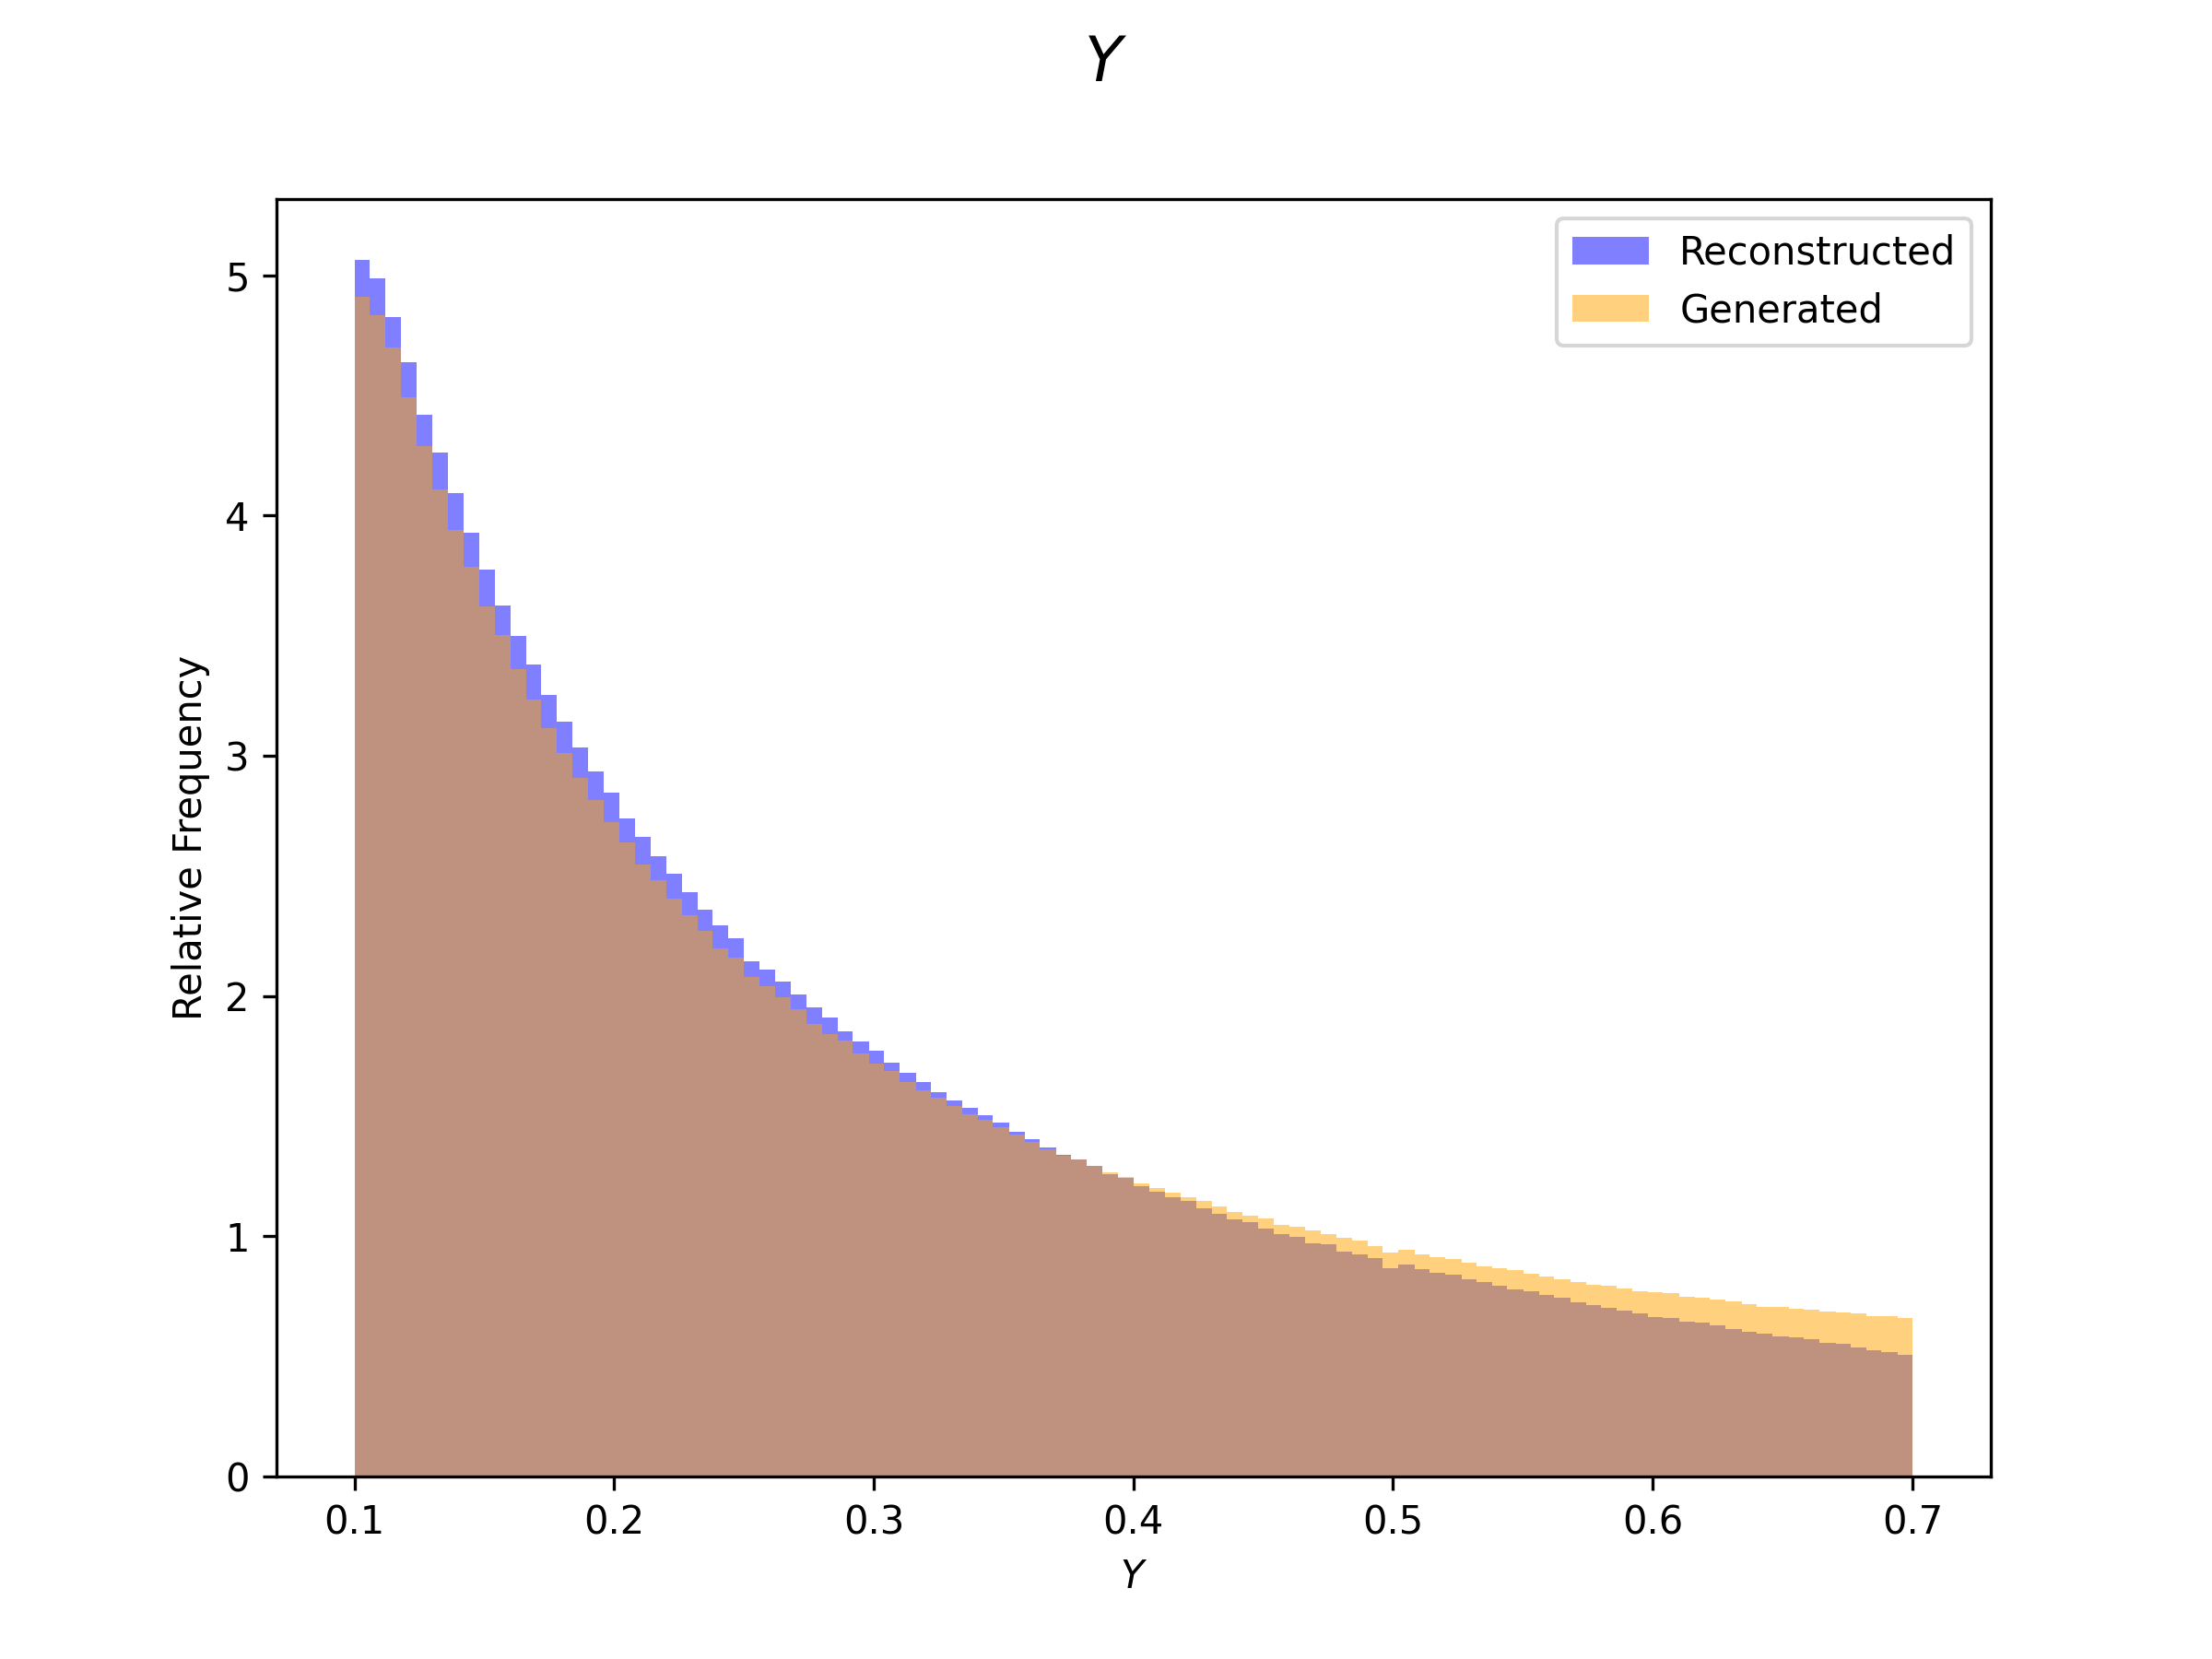
\includegraphics[width=\textwidth]{graphs/incl_Y.png}
        \caption{Histogram for $Y$}
        \label{fig:incl_Y}
    \end{subfigure}
    \caption{Histograms for $X_b$ and $Y$}
\end{figure}

\begin{figure}[H]
    \centering
    \begin{subfigure}[b]{0.45\textwidth}
        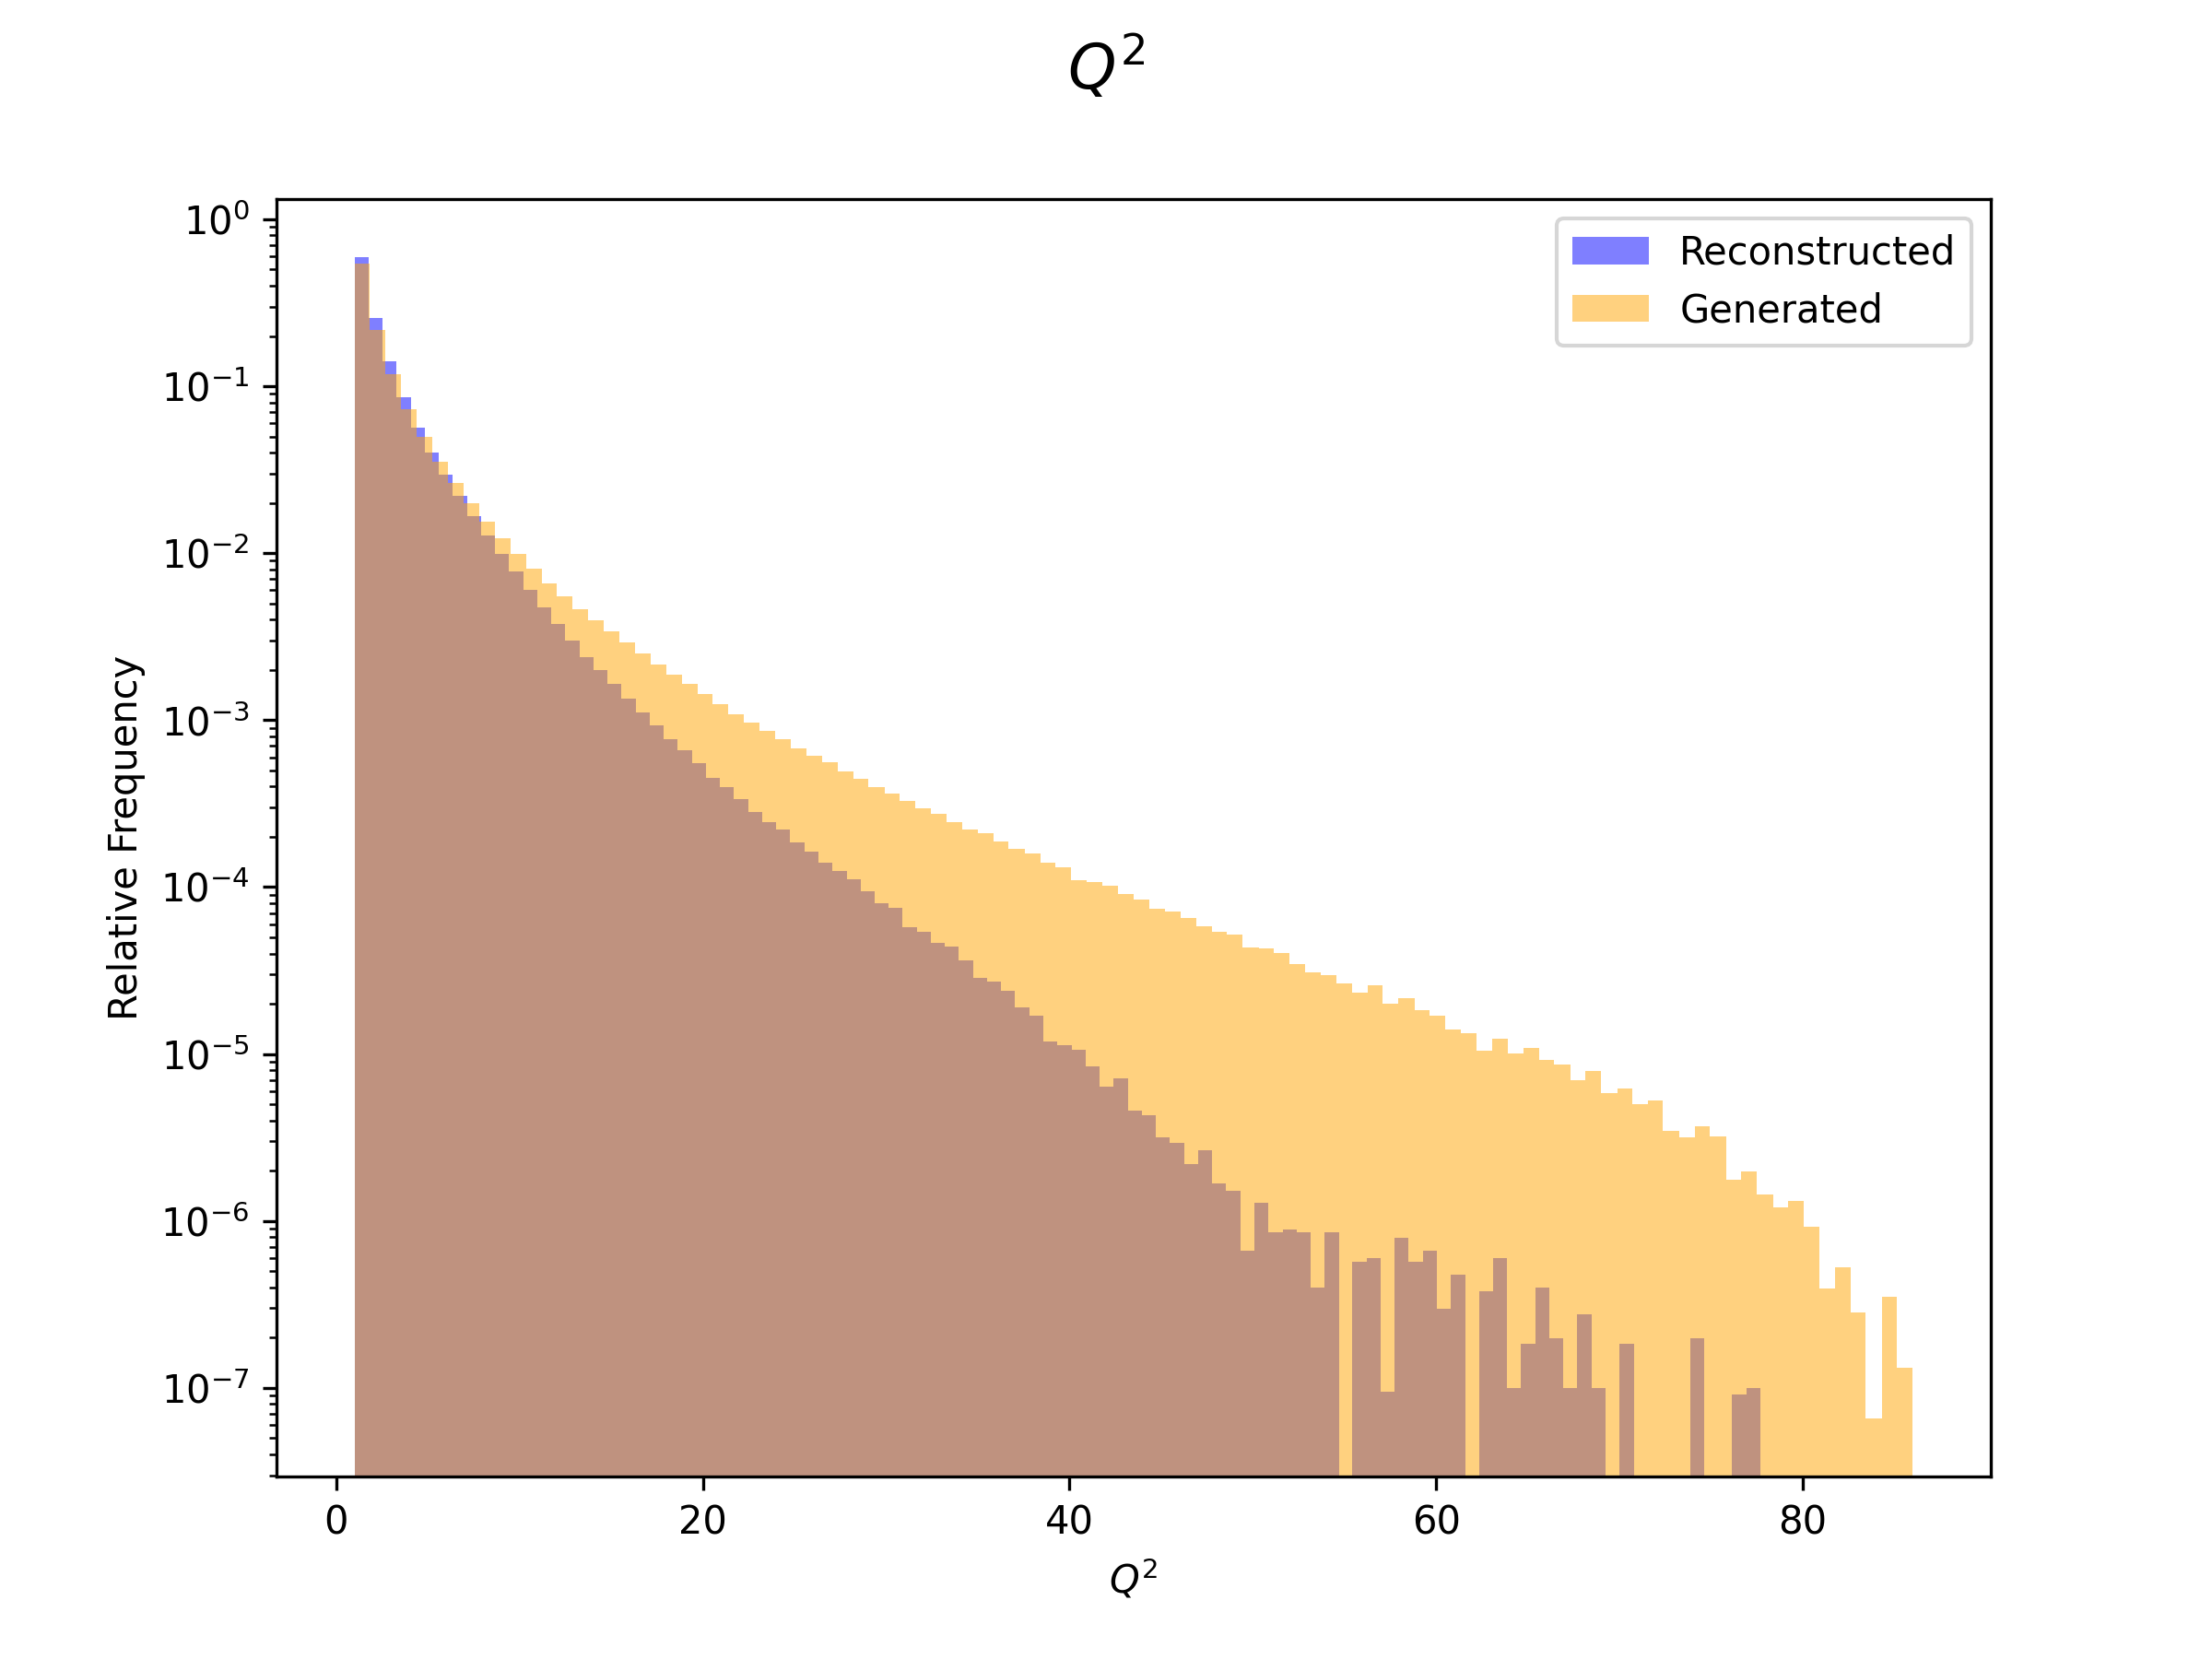
\includegraphics[width=\textwidth]{graphs/incl_Q2.png}
        \caption{Histogram for $Q^2$}
        \label{fig:incl_Q2}
    \end{subfigure}
    \hfill
    \begin{subfigure}[b]{0.45\textwidth}
        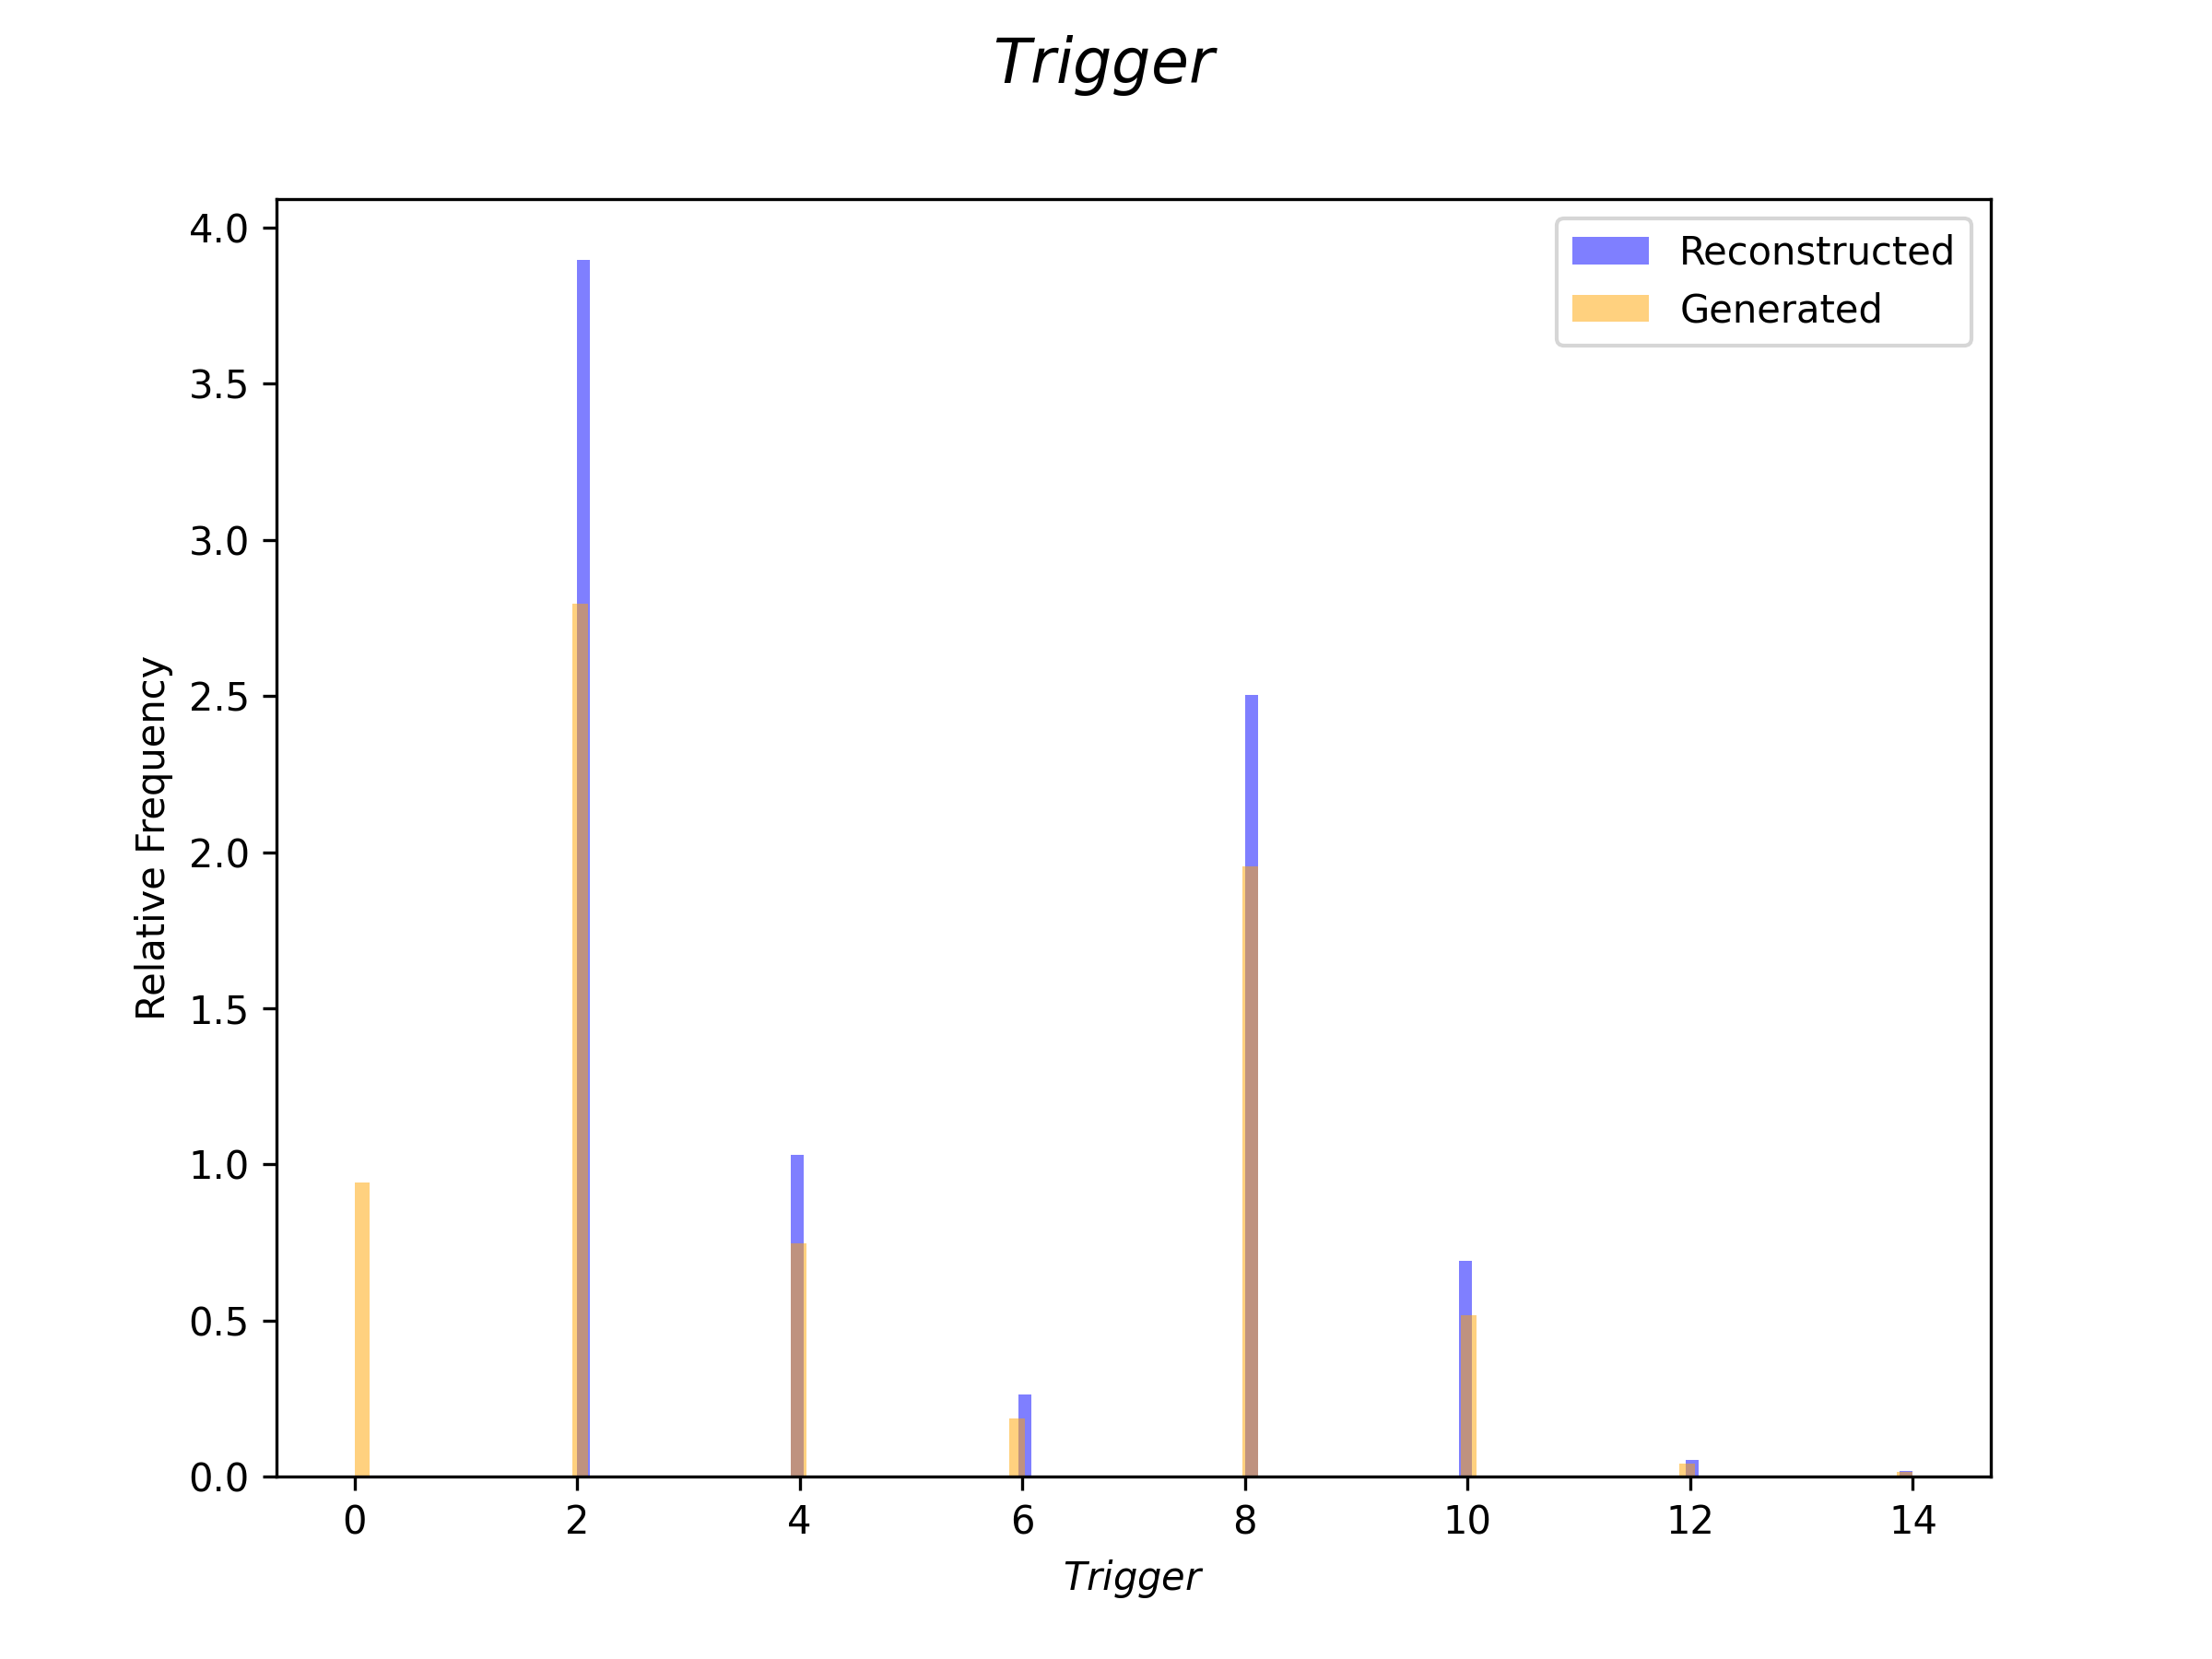
\includegraphics[width=\textwidth]{graphs/incl_Trigger.png}
        \caption{Histogram for $Trigger$}
        \label{fig:incl_Trig}
    \end{subfigure}
    \caption{Histograms for $Q^2$ and $Trig$}
\end{figure}

\begin{figure}[H]
    \centering
    \begin{subfigure}[b]{0.45\textwidth}
        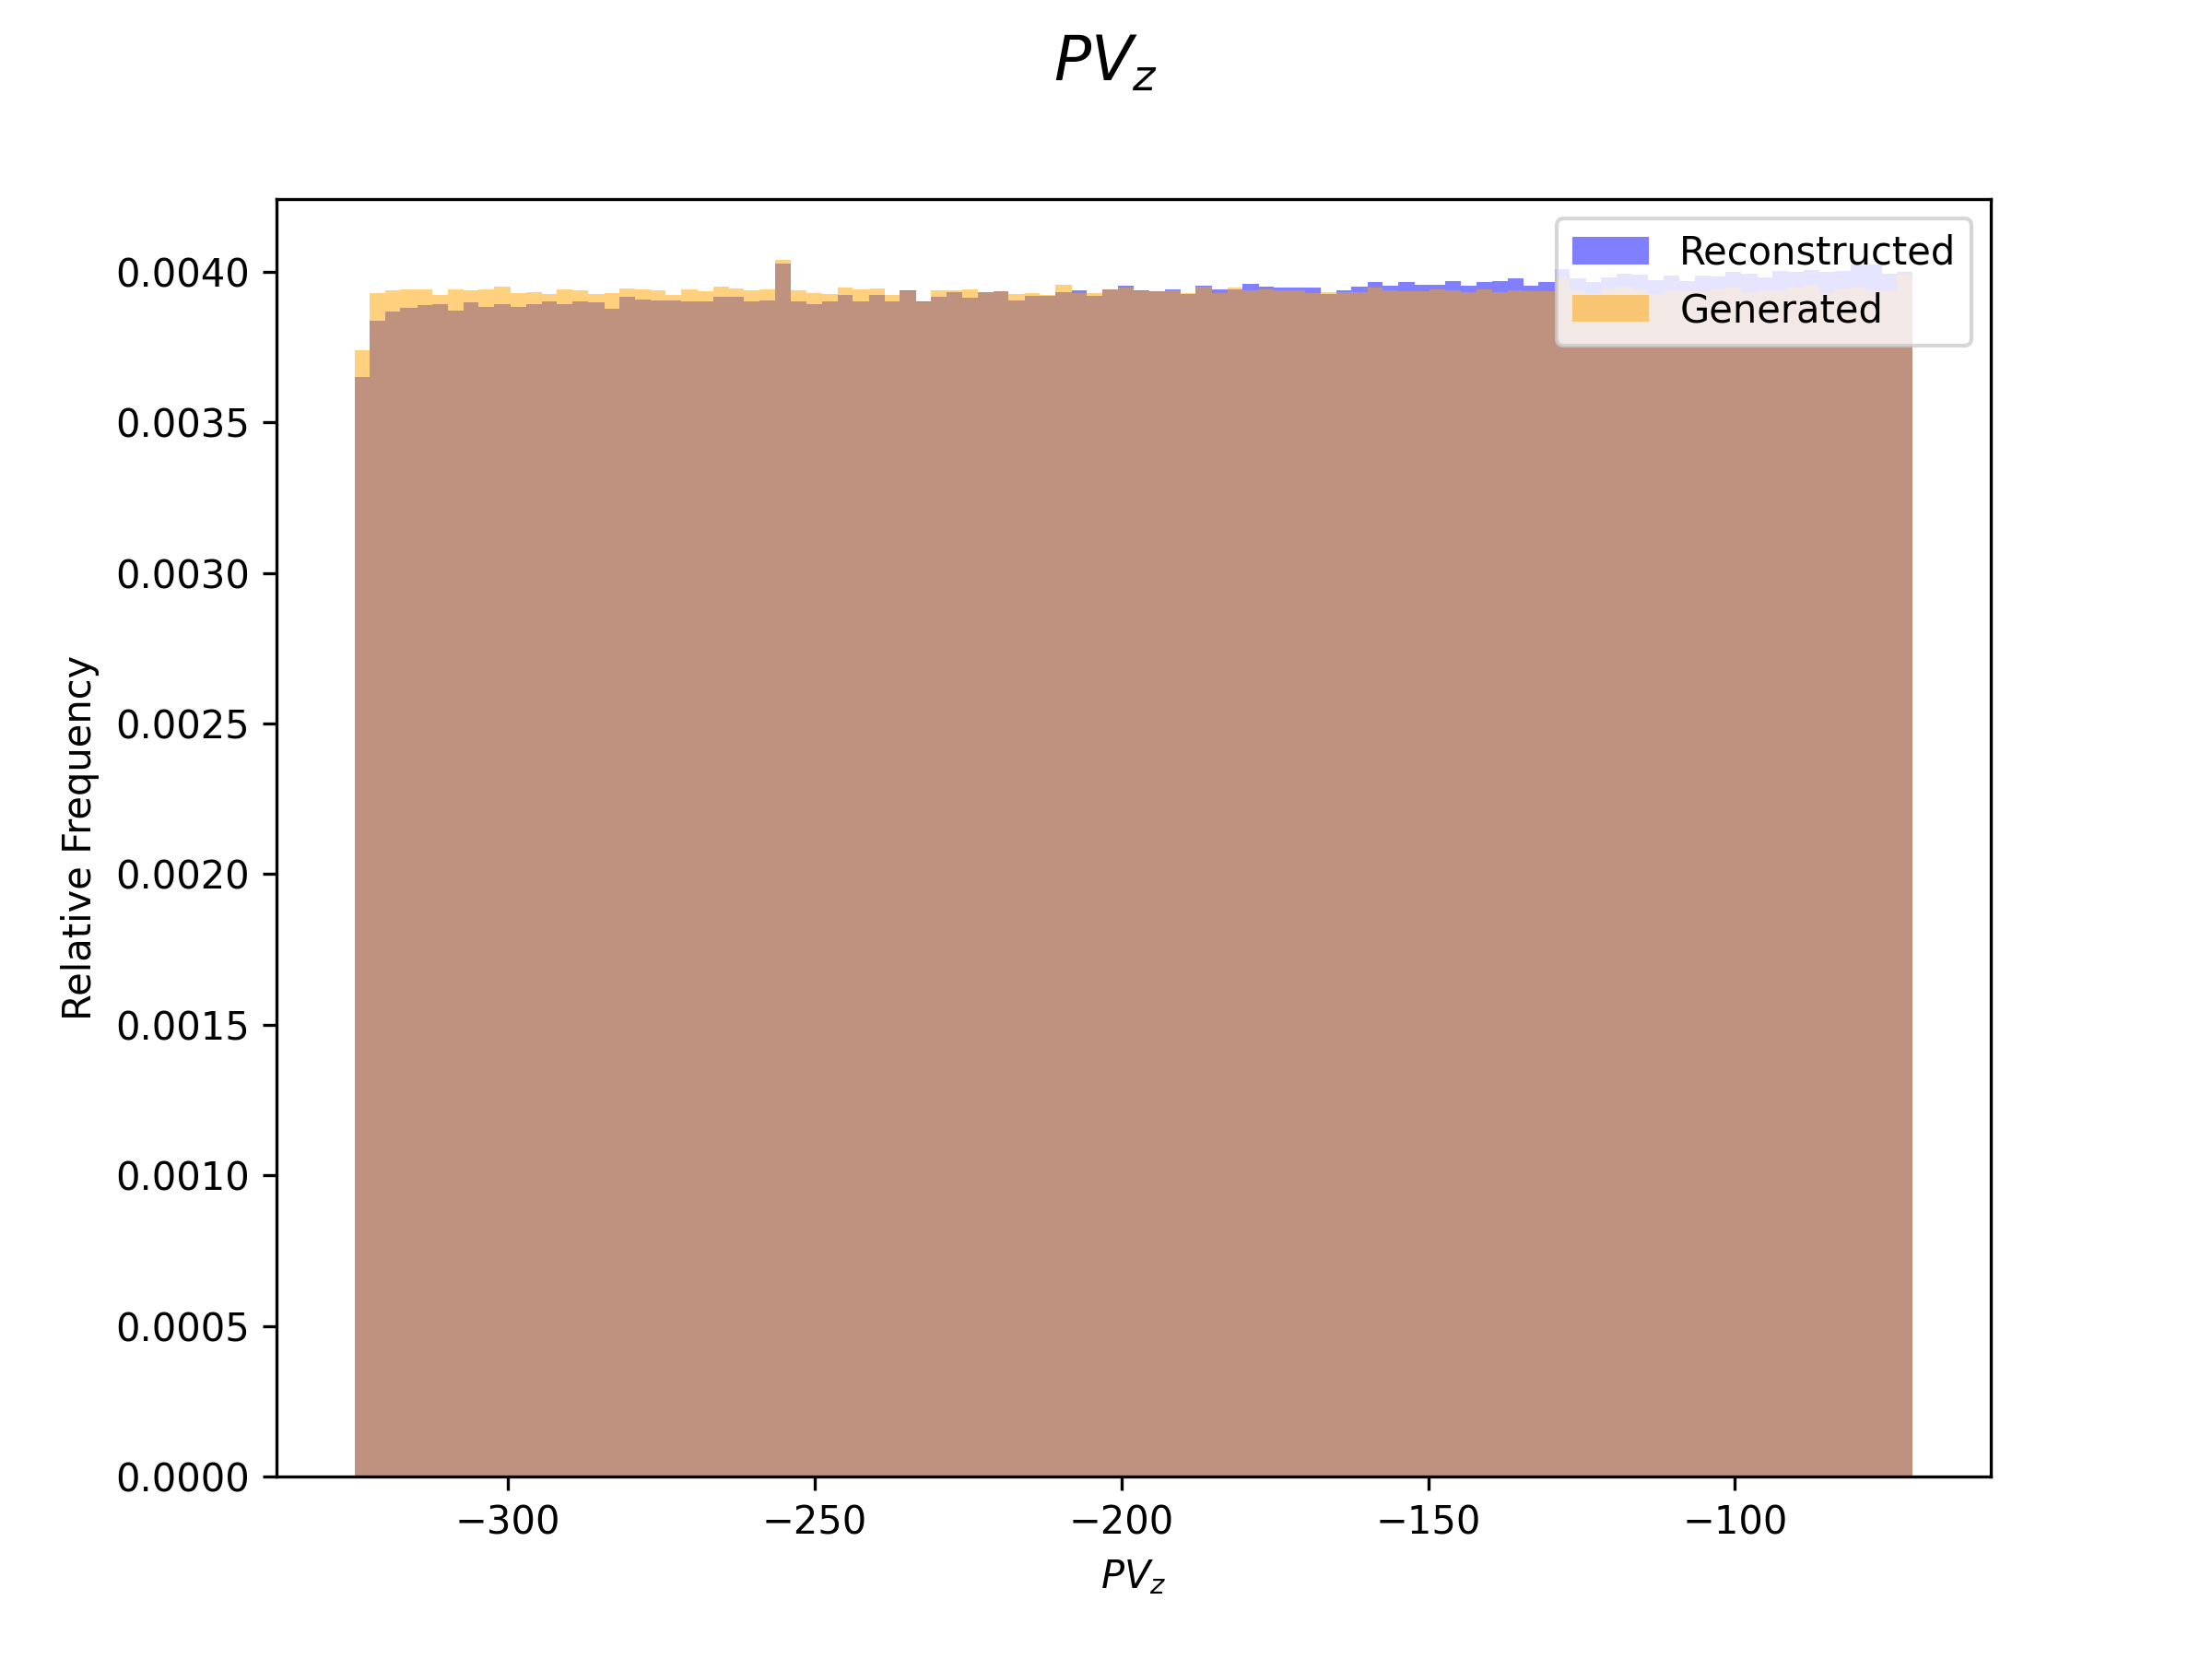
\includegraphics[width=\textwidth]{graphs/incl_PV_z.png}
        \caption{Histogram for $PV_z$}
        \label{fig:incl_PV_z}
    \end{subfigure}
    \hfill
    \begin{subfigure}[b]{0.45\textwidth}
        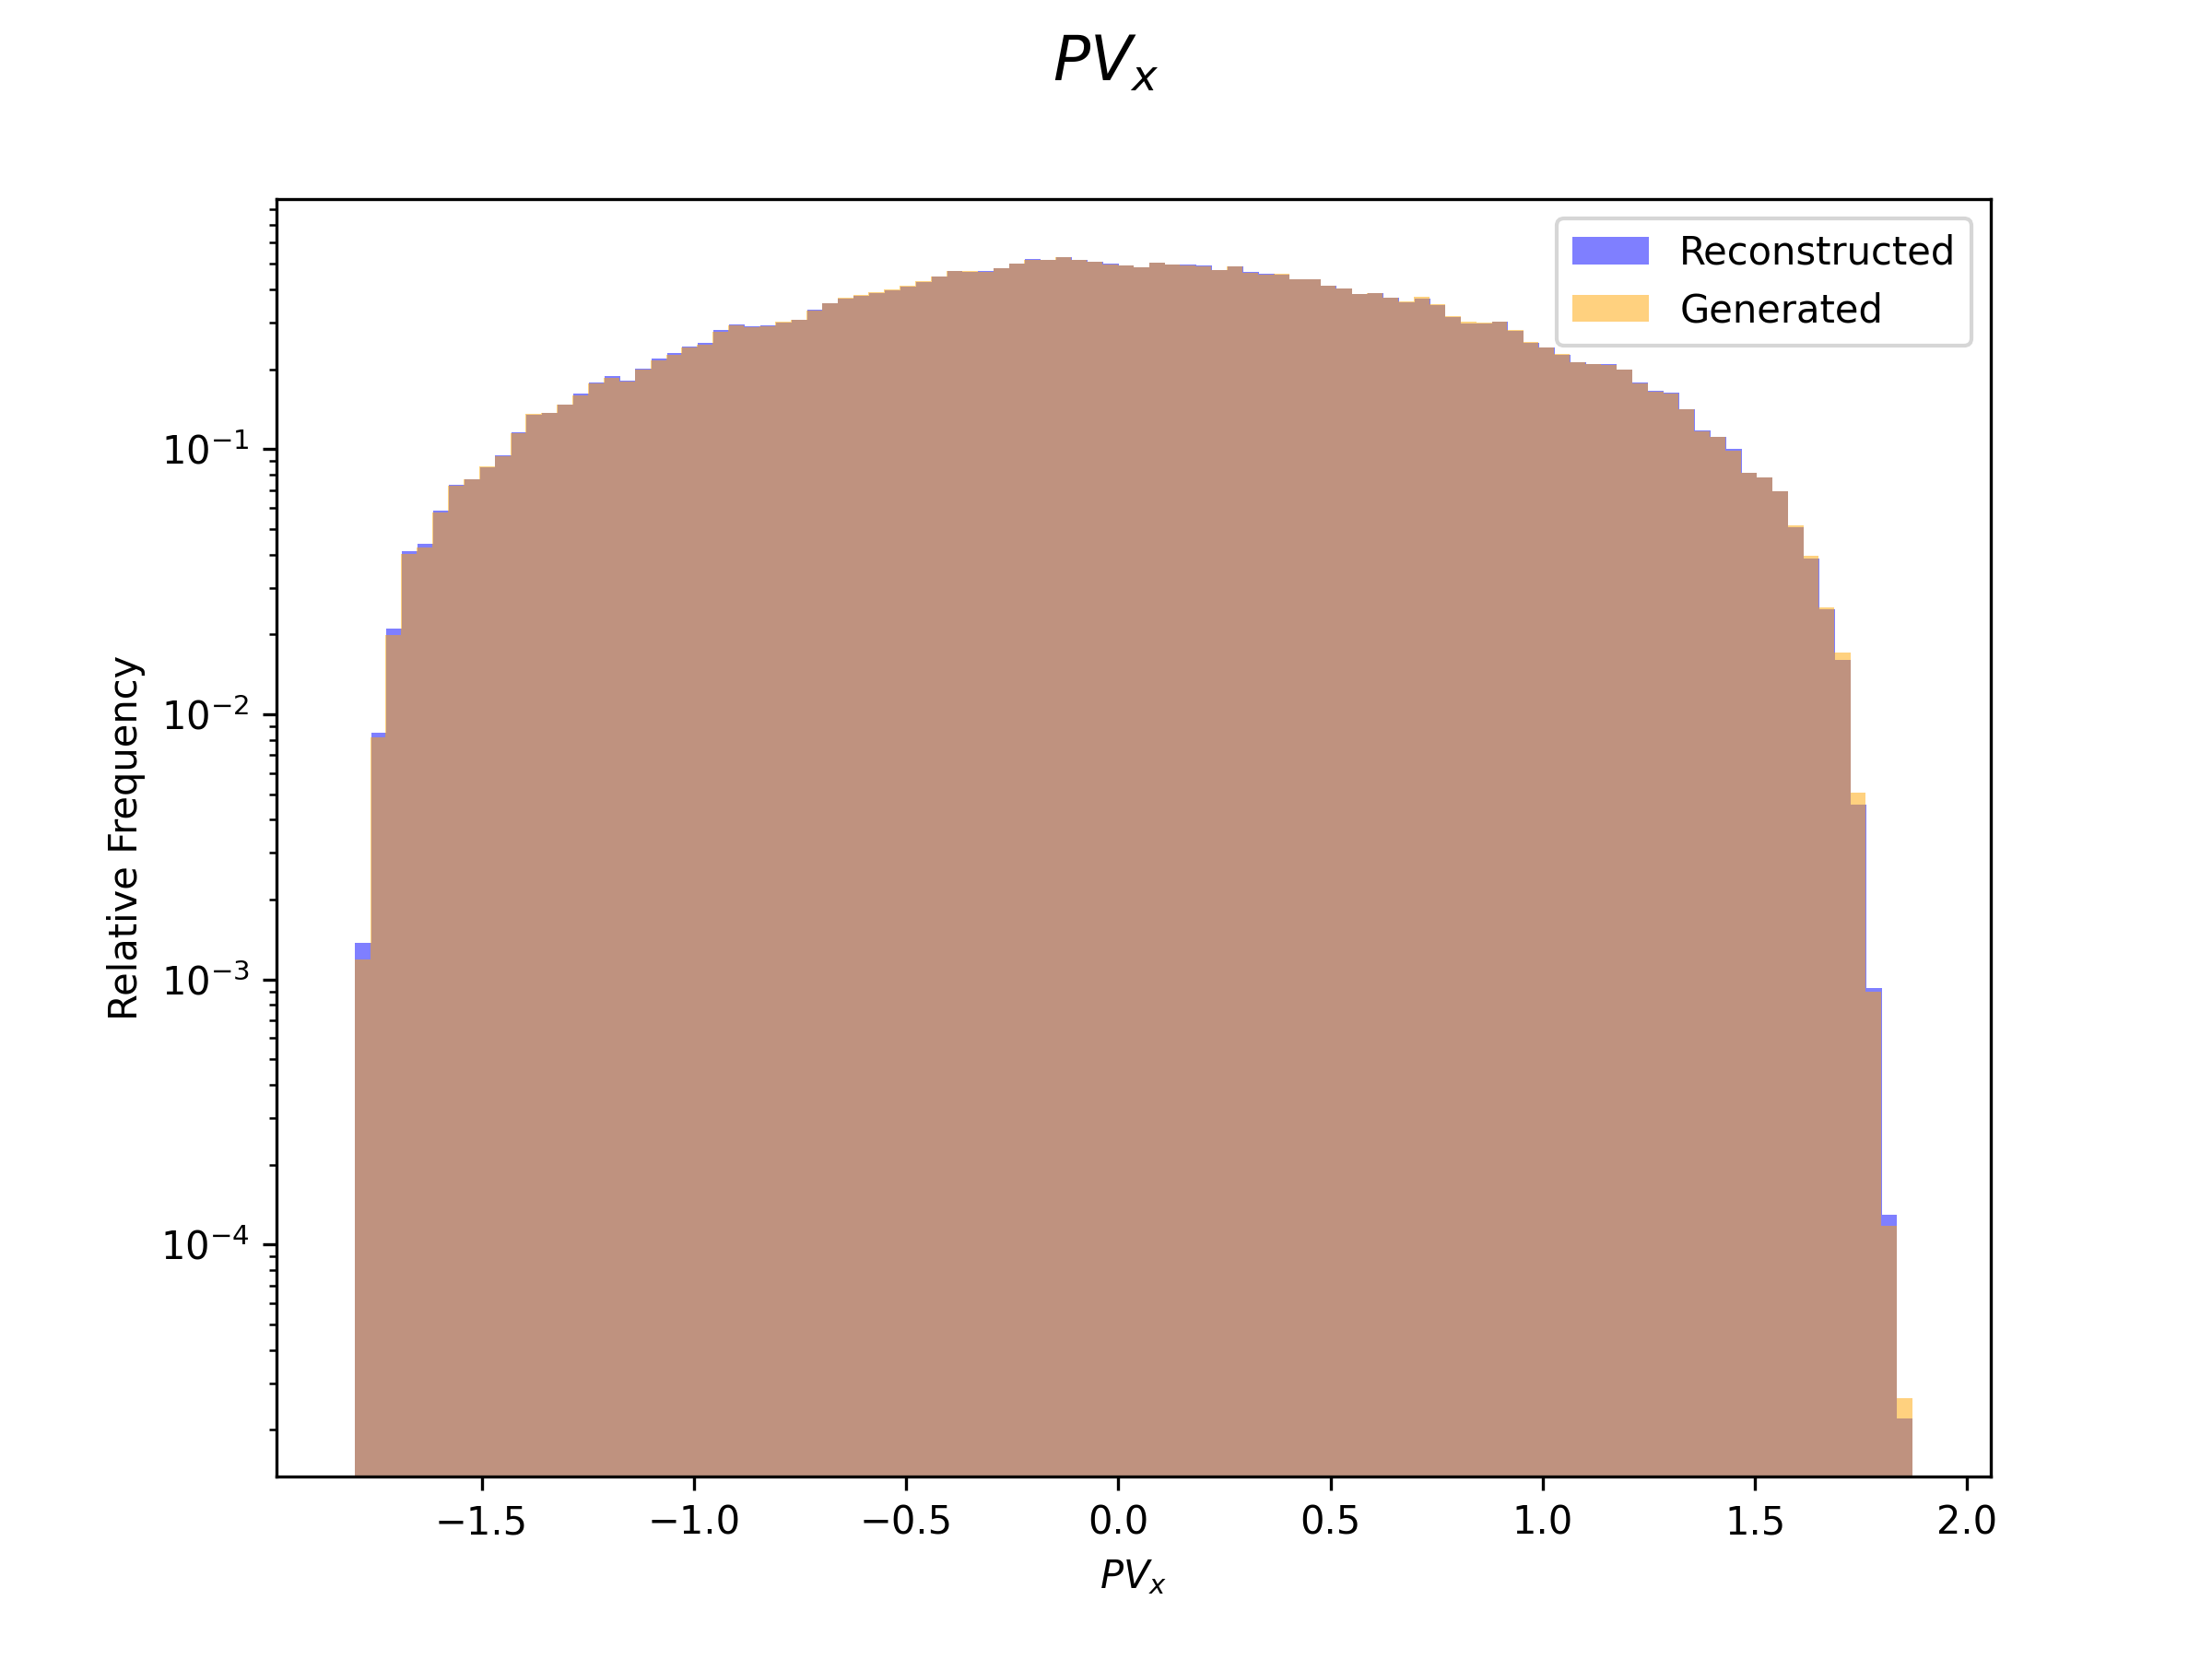
\includegraphics[width=\textwidth]{graphs/incl_PV_x.png}
        \caption{Histogram for $PV_x$}
        \label{fig:incl_PV_x}
    \end{subfigure}
    \caption{Histograms for $PV_z$ and $PV_x$}
\end{figure}

\begin{figure}[H]
    \centering
    \begin{subfigure}[b]{0.45\textwidth}
        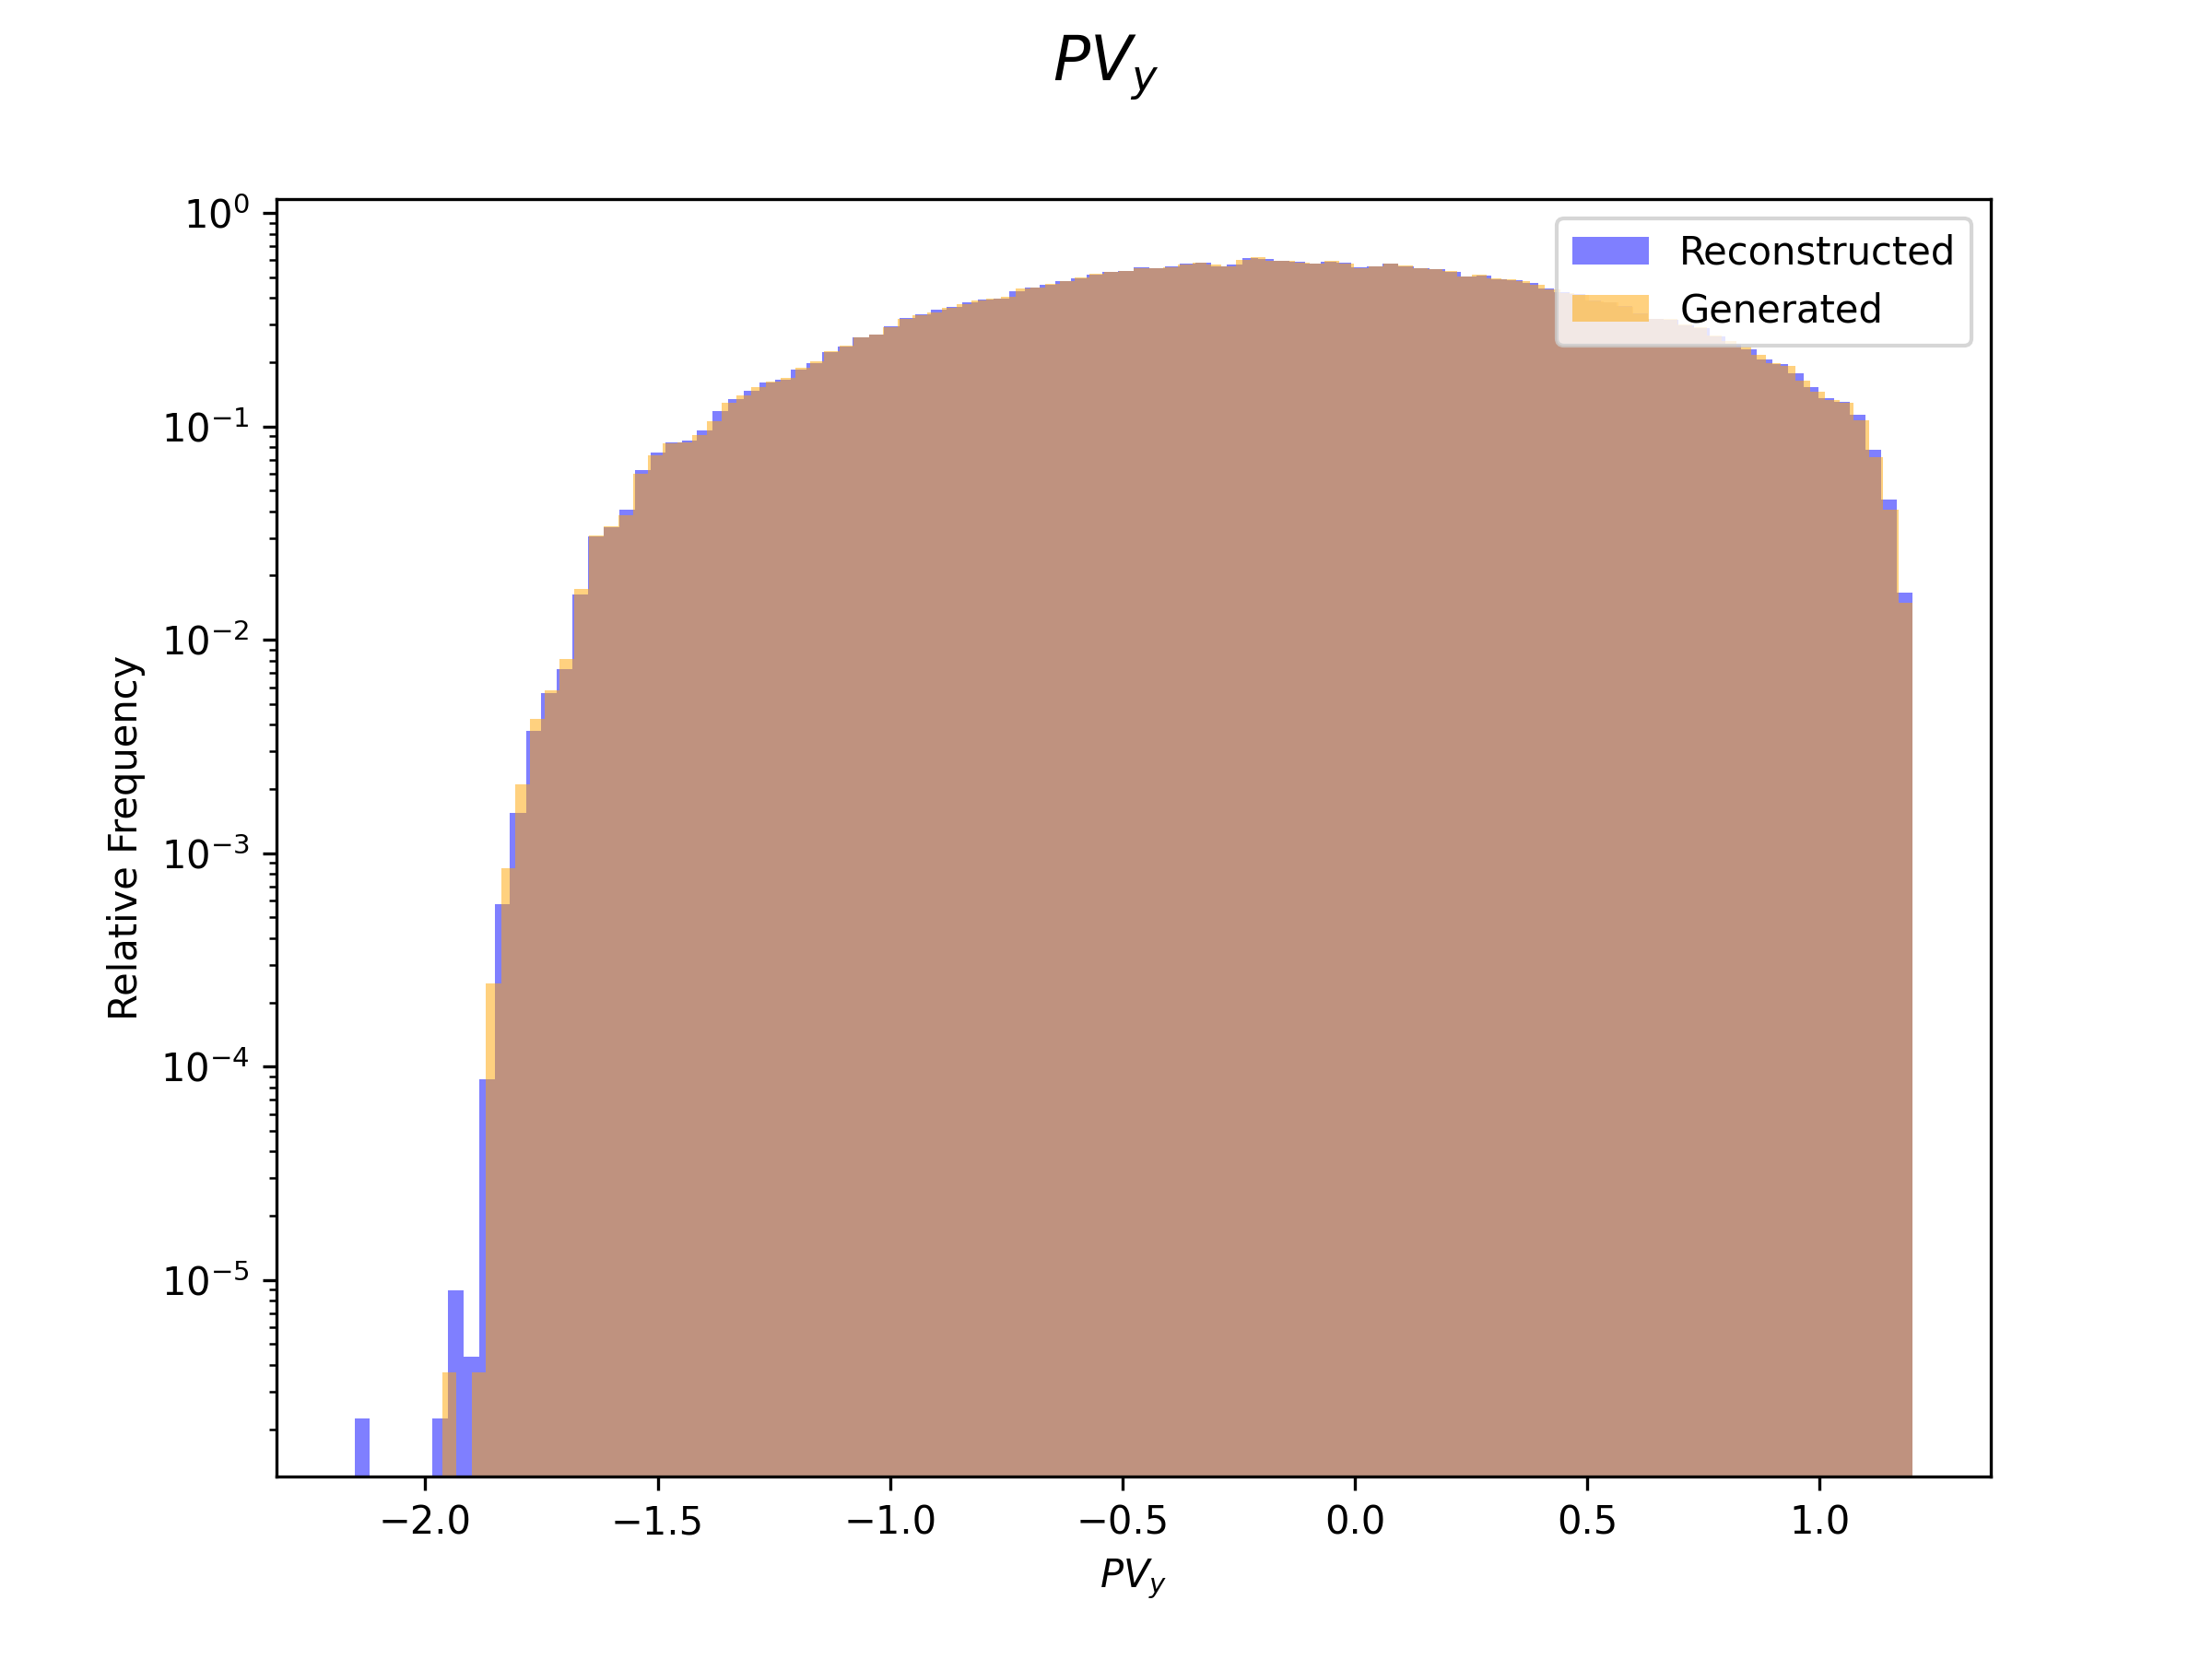
\includegraphics[width=\textwidth]{graphs/incl_PV_y.png}
        \caption{Histogram for $PV_y$}
        \label{fig:incl_PV_y}
    \end{subfigure}
    \hfill
    \begin{subfigure}[b]{0.45\textwidth}
        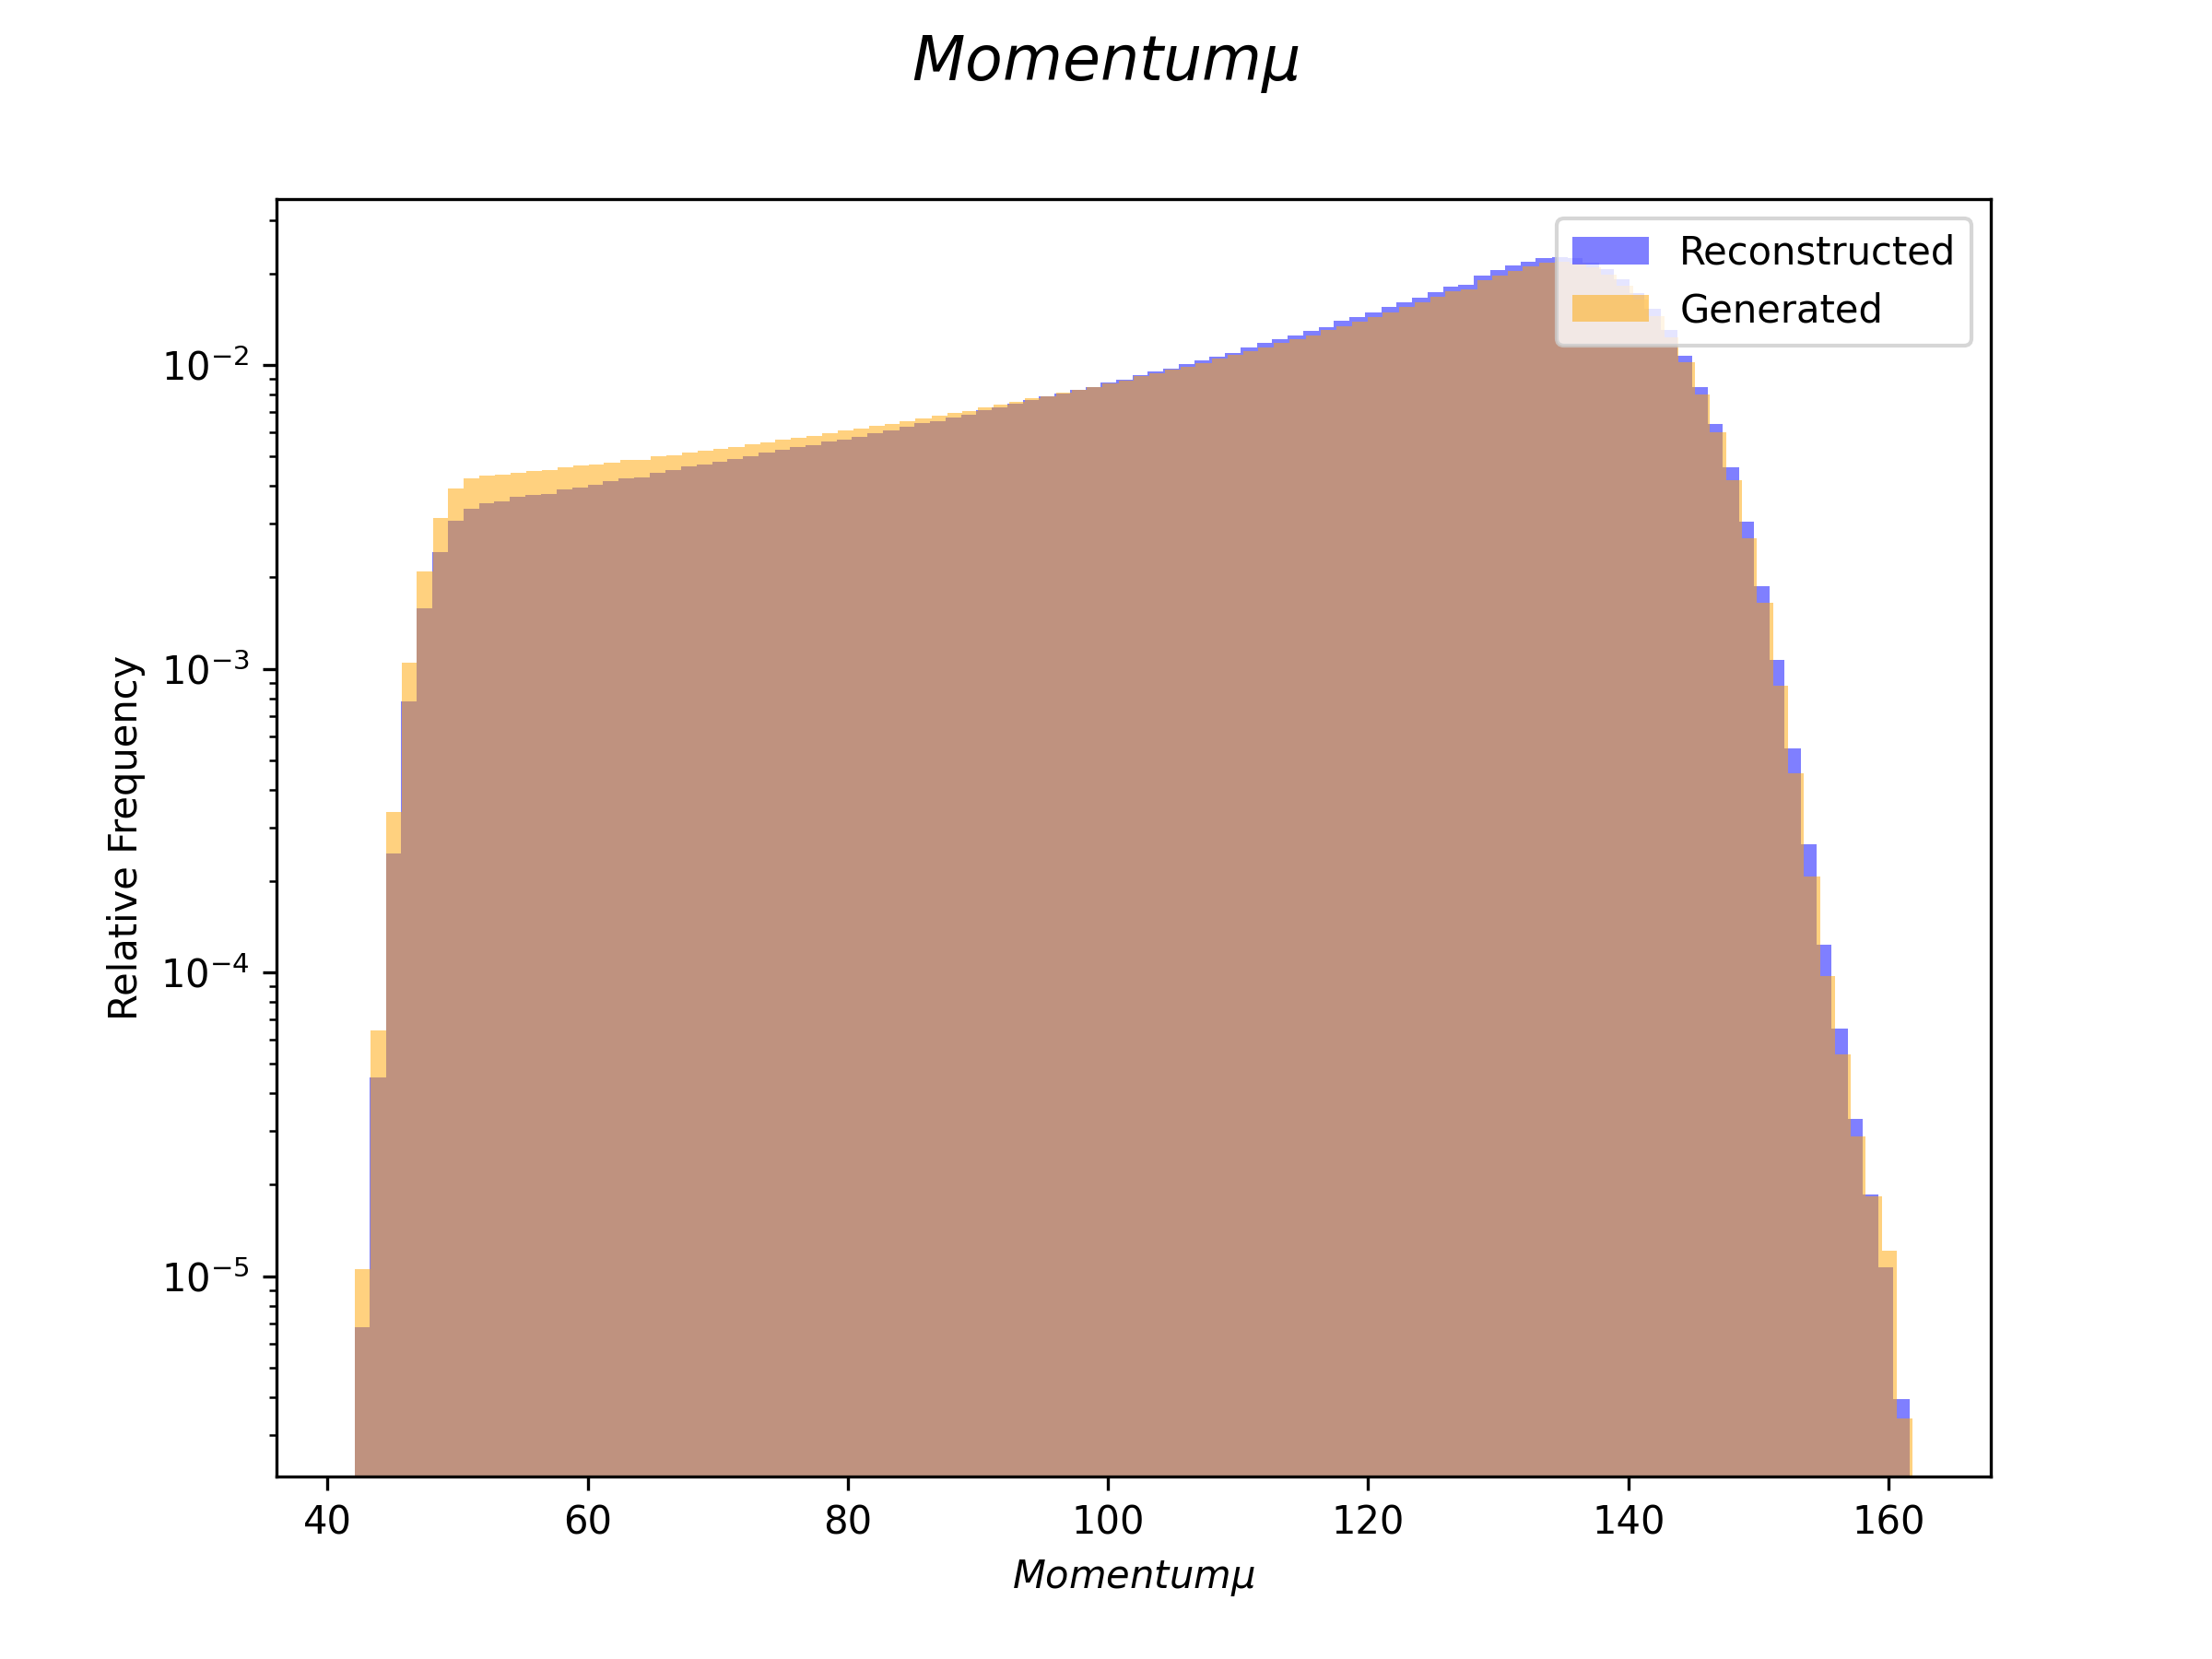
\includegraphics[width=\textwidth]{graphs/incl_Momentum_mu.png}
        \caption{Histogram for $Mom_{mu}$}
        \label{fig:incl_Momentum_mu}
    \end{subfigure}
    \caption{Histograms for $PV_y$ and $Mom_{mu}$}
\end{figure}

\begin{figure}[H]
    \centering
    \begin{subfigure}[b]{0.45\textwidth}
        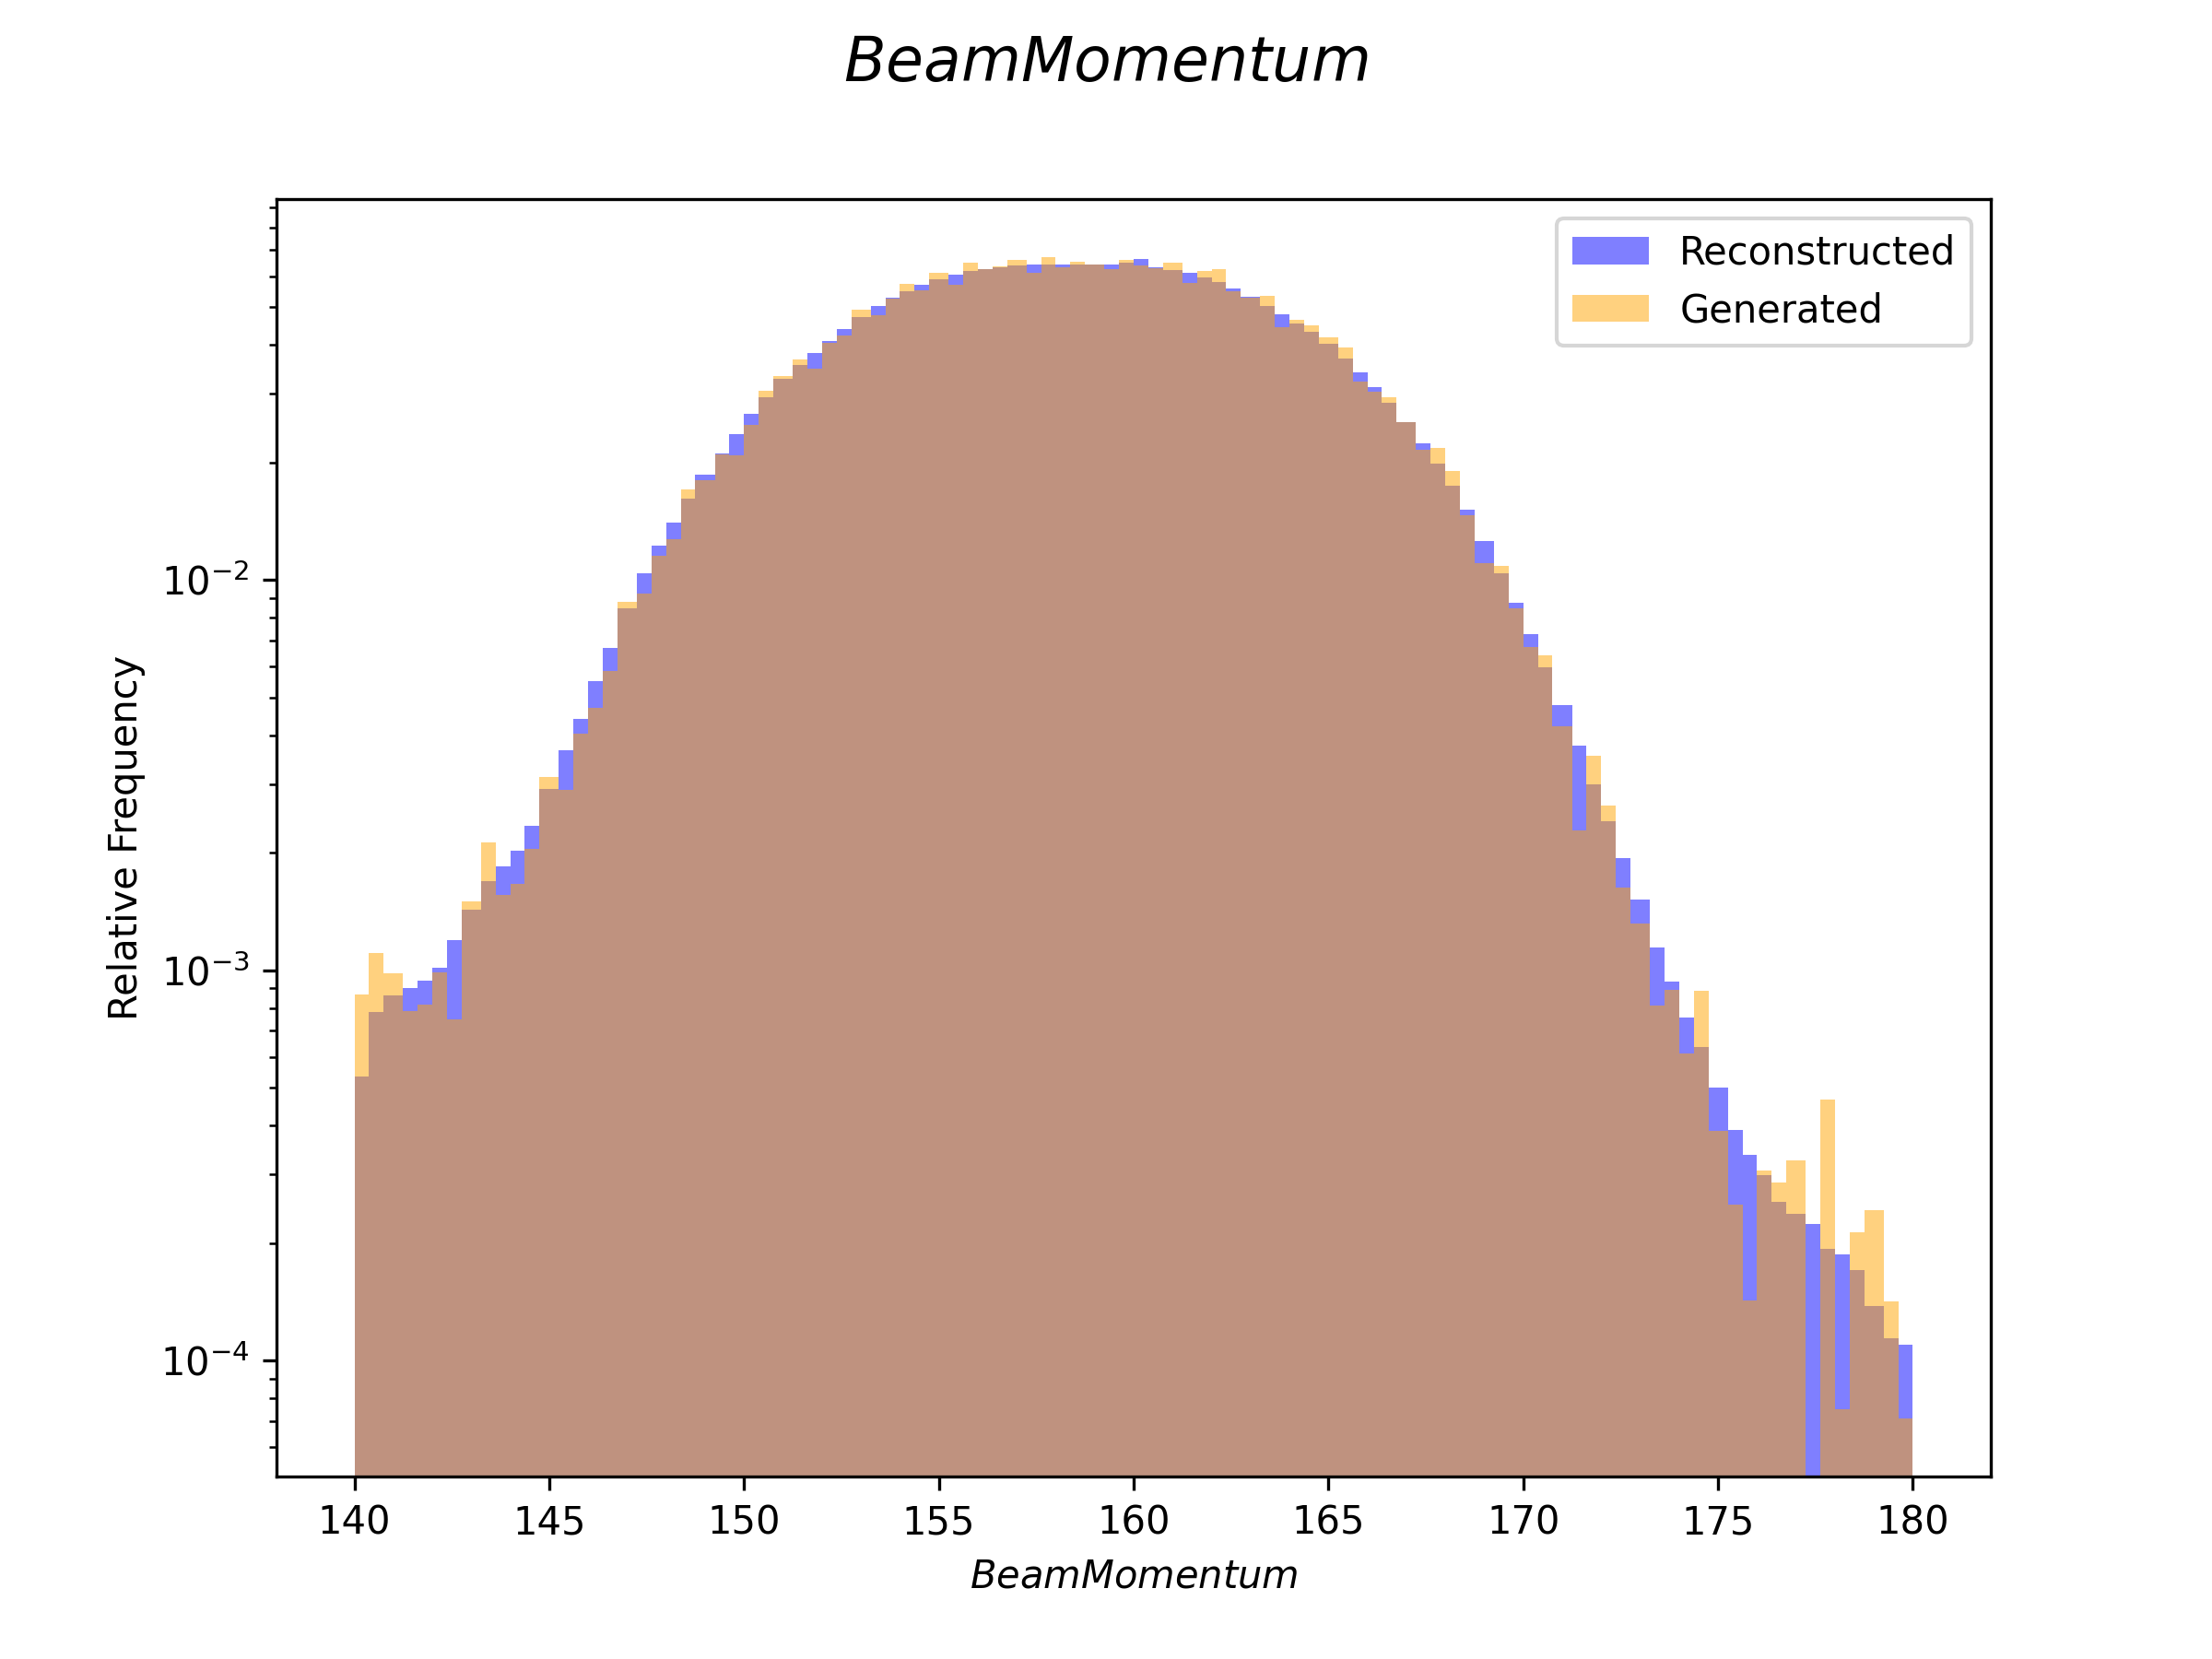
\includegraphics[width=\textwidth]{graphs/incl_Beam_Momentum.png}
        \caption{Histogram for $Mom_{mup}$}
        \label{fig:incl_Momentum_mup}
    \end{subfigure}
    \hfill
    \begin{subfigure}[b]{0.45\textwidth}
        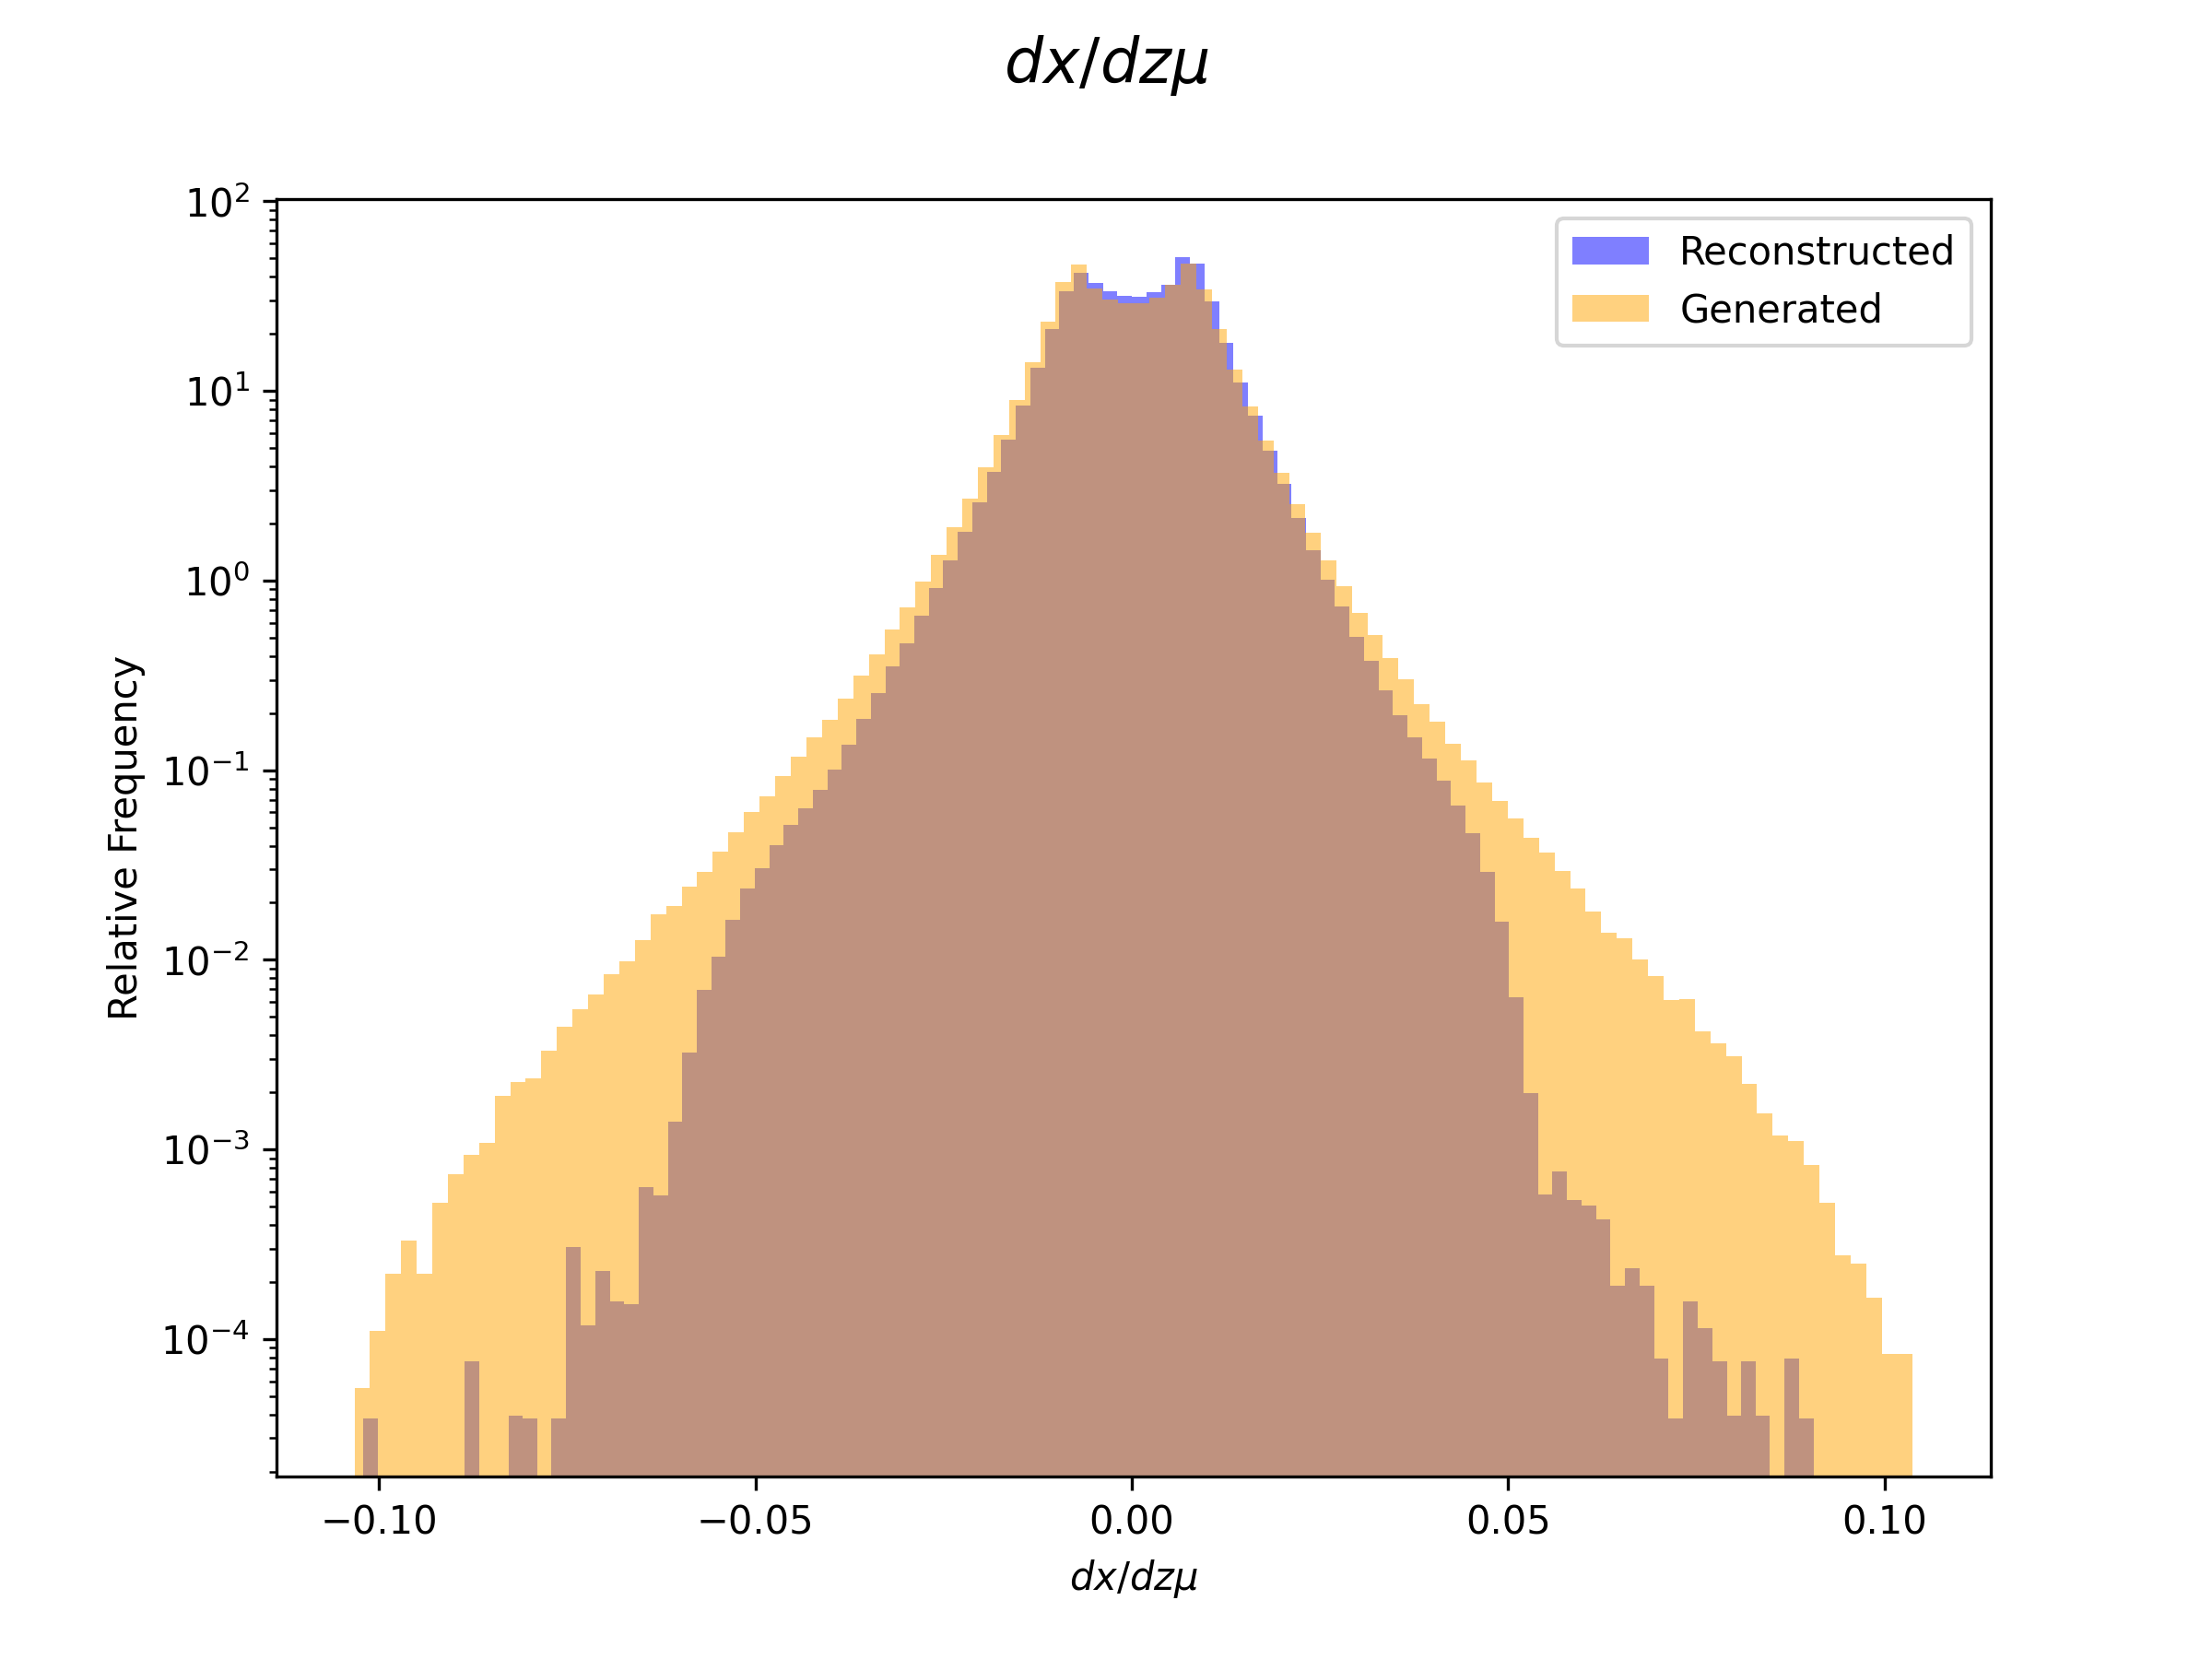
\includegraphics[width=\textwidth]{graphs/incl_dx_dz_mu.png}
        \caption{Histogram for $d_xd_zmup$}
        \label{fig:incl_Angle_mu_1}
    \end{subfigure}
    \caption{Histograms for $Mom_{mup}$ and $d_xd_zmup$}
\end{figure}

\begin{figure}[H]
    \centering
    \begin{subfigure}[b]{0.45\textwidth}
        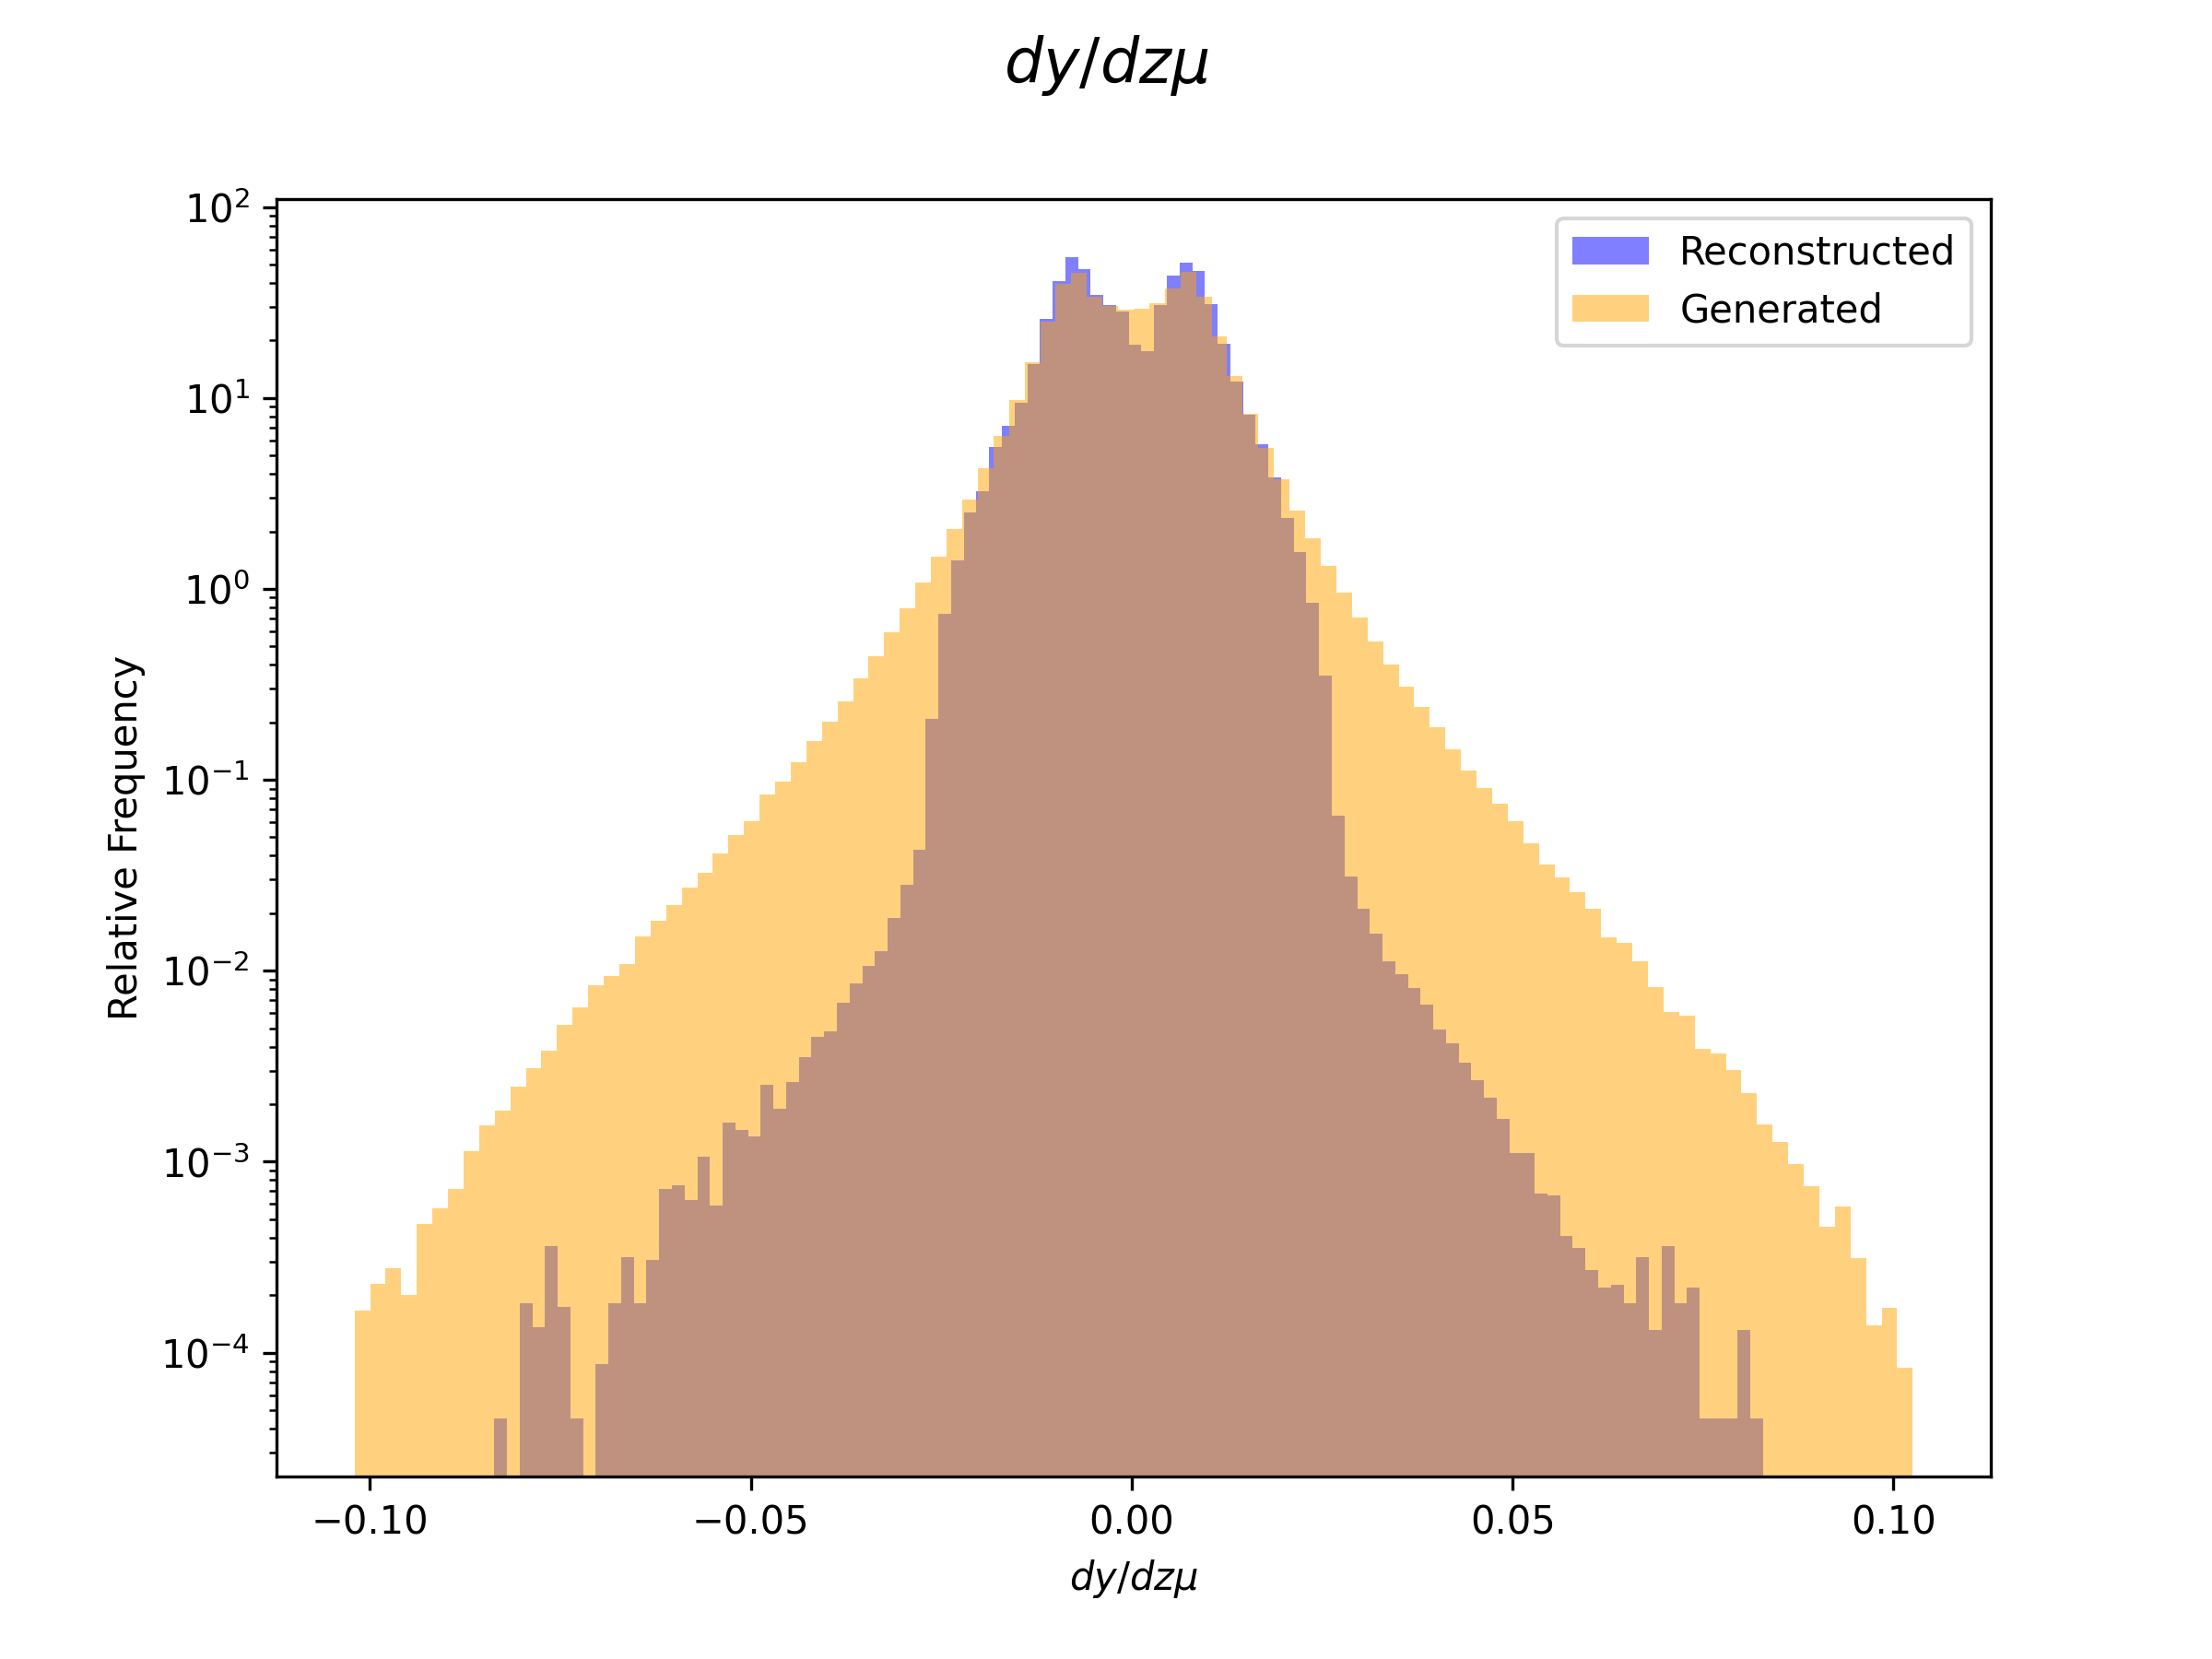
\includegraphics[width=\textwidth]{graphs/incl_dy_dz_mu.png}
        \caption{Histogram for $d_yd_zmup$}
        \label{fig:incl_Angle_mu}
    \end{subfigure}
    \caption{Histogram for $d_yd_zmup$}
\end{figure}

Since we're going to use a 2D histogram for the chi-squared test to further evaluate the performance of the models (explained in section METER AQUI), we plotted the 2D histogram for the $X$ and $Y$ variables for the Inclusive:

\begin{figure}[H]
    \centering
    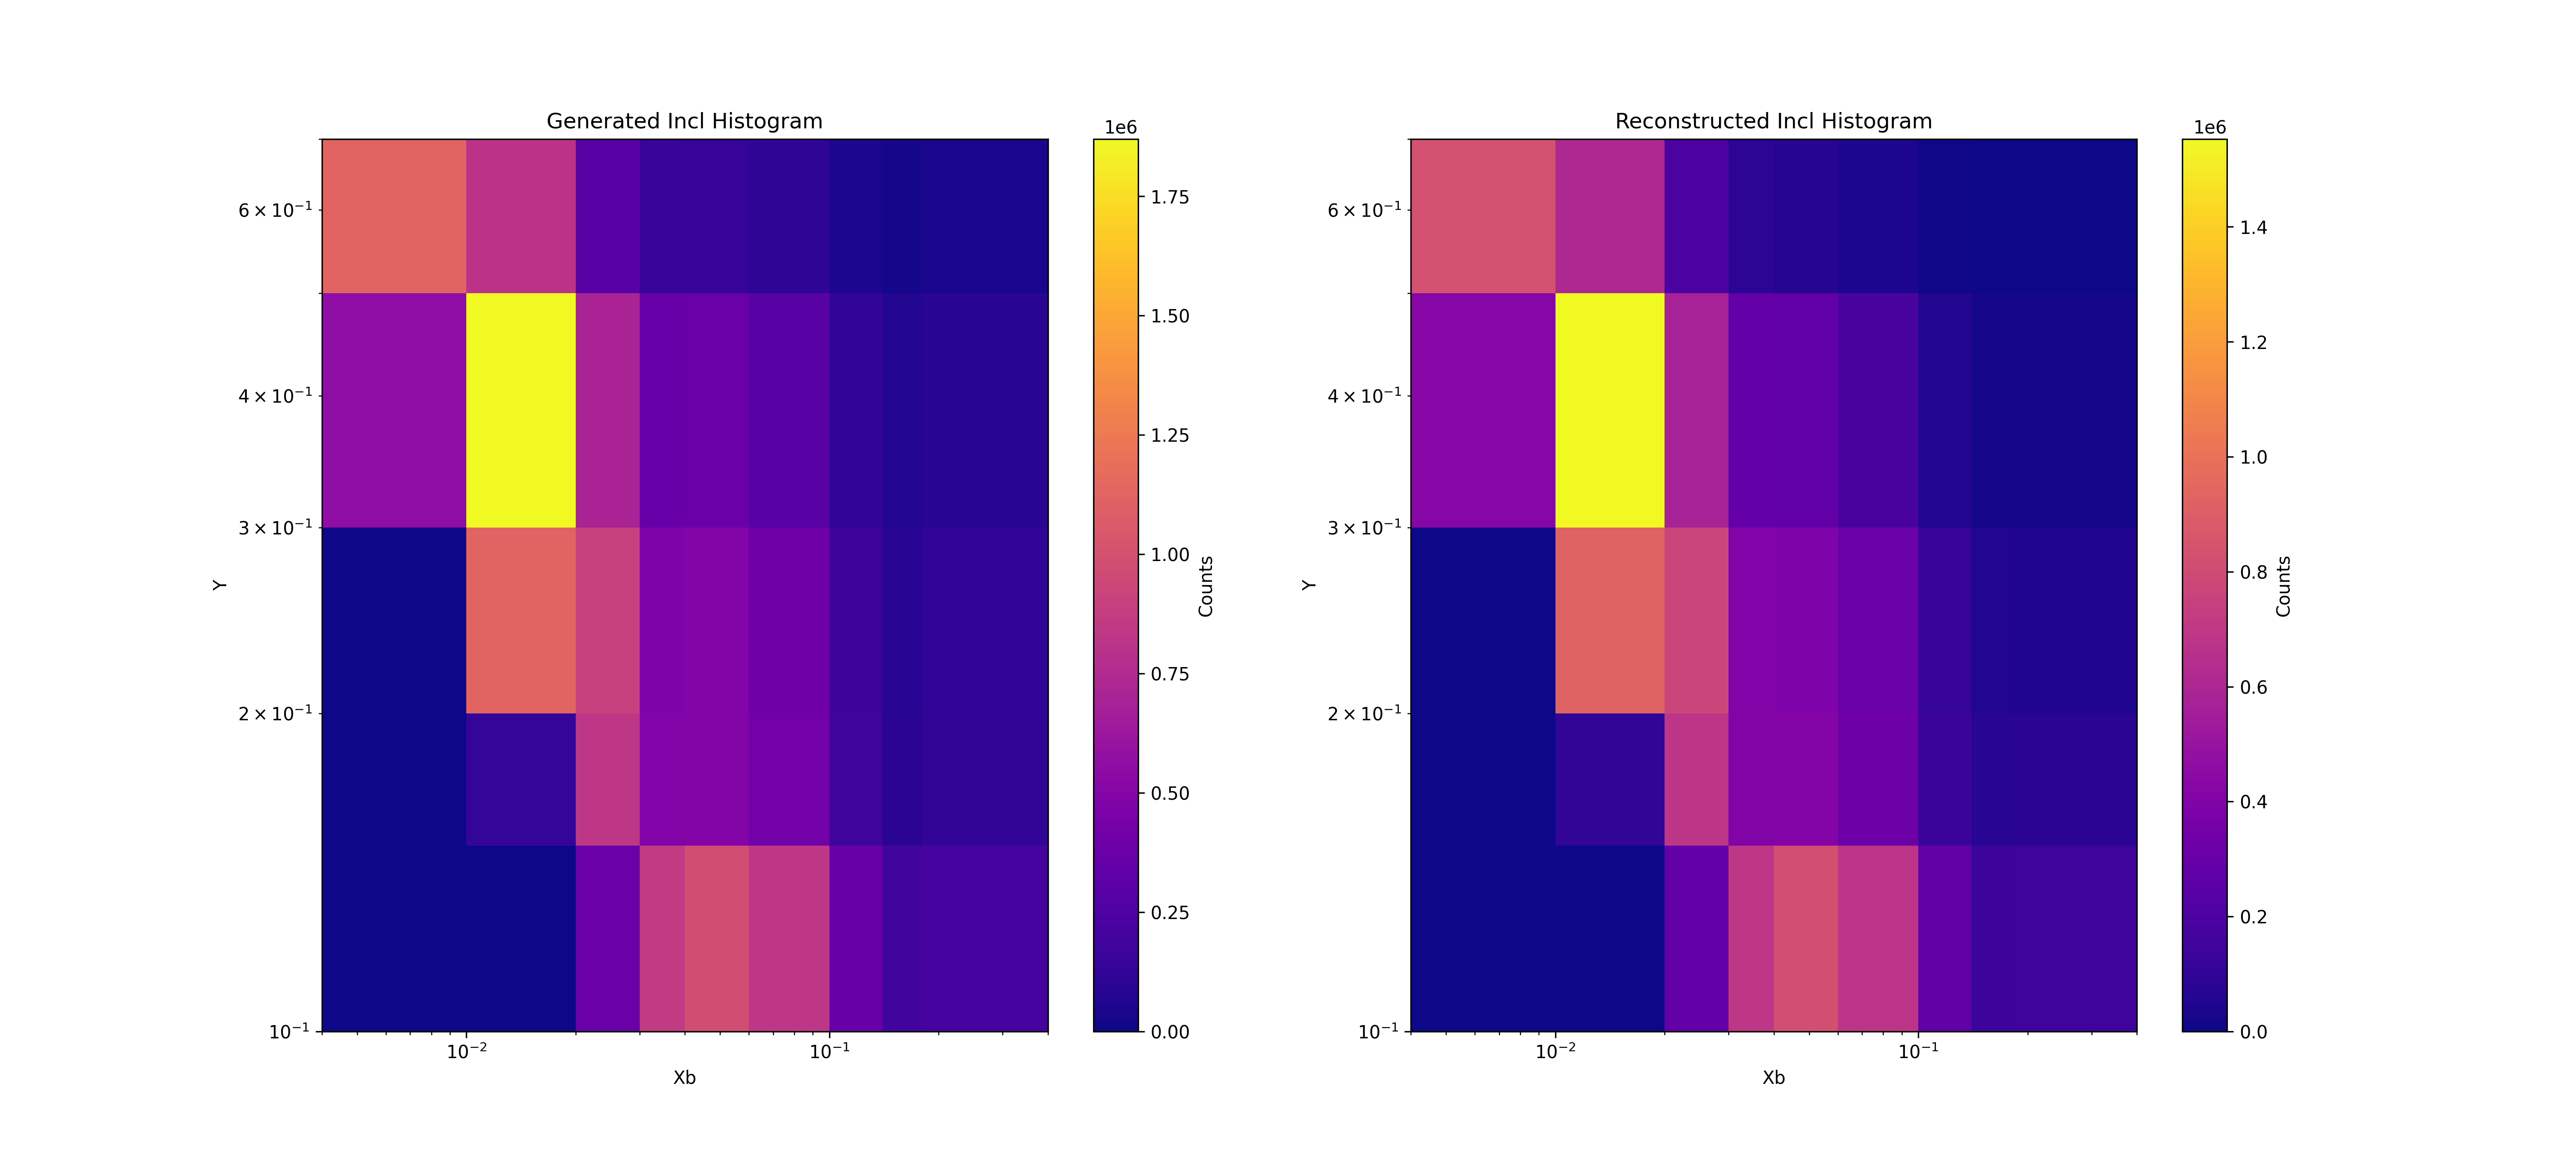
\includegraphics[width=0.9\textwidth]{graphs/incl_xb_y.png}
    \caption{2D Histogram with $X$ and $Y$ for the Inclusive Events}
    \label{fig:inclusive_2D_histogram}
\end{figure}

\textbf{The histograms for the Hadrons events are shown in the figures below:}

\begin{figure}[H]
    \centering
    \begin{subfigure}[b]{0.45\textwidth}
        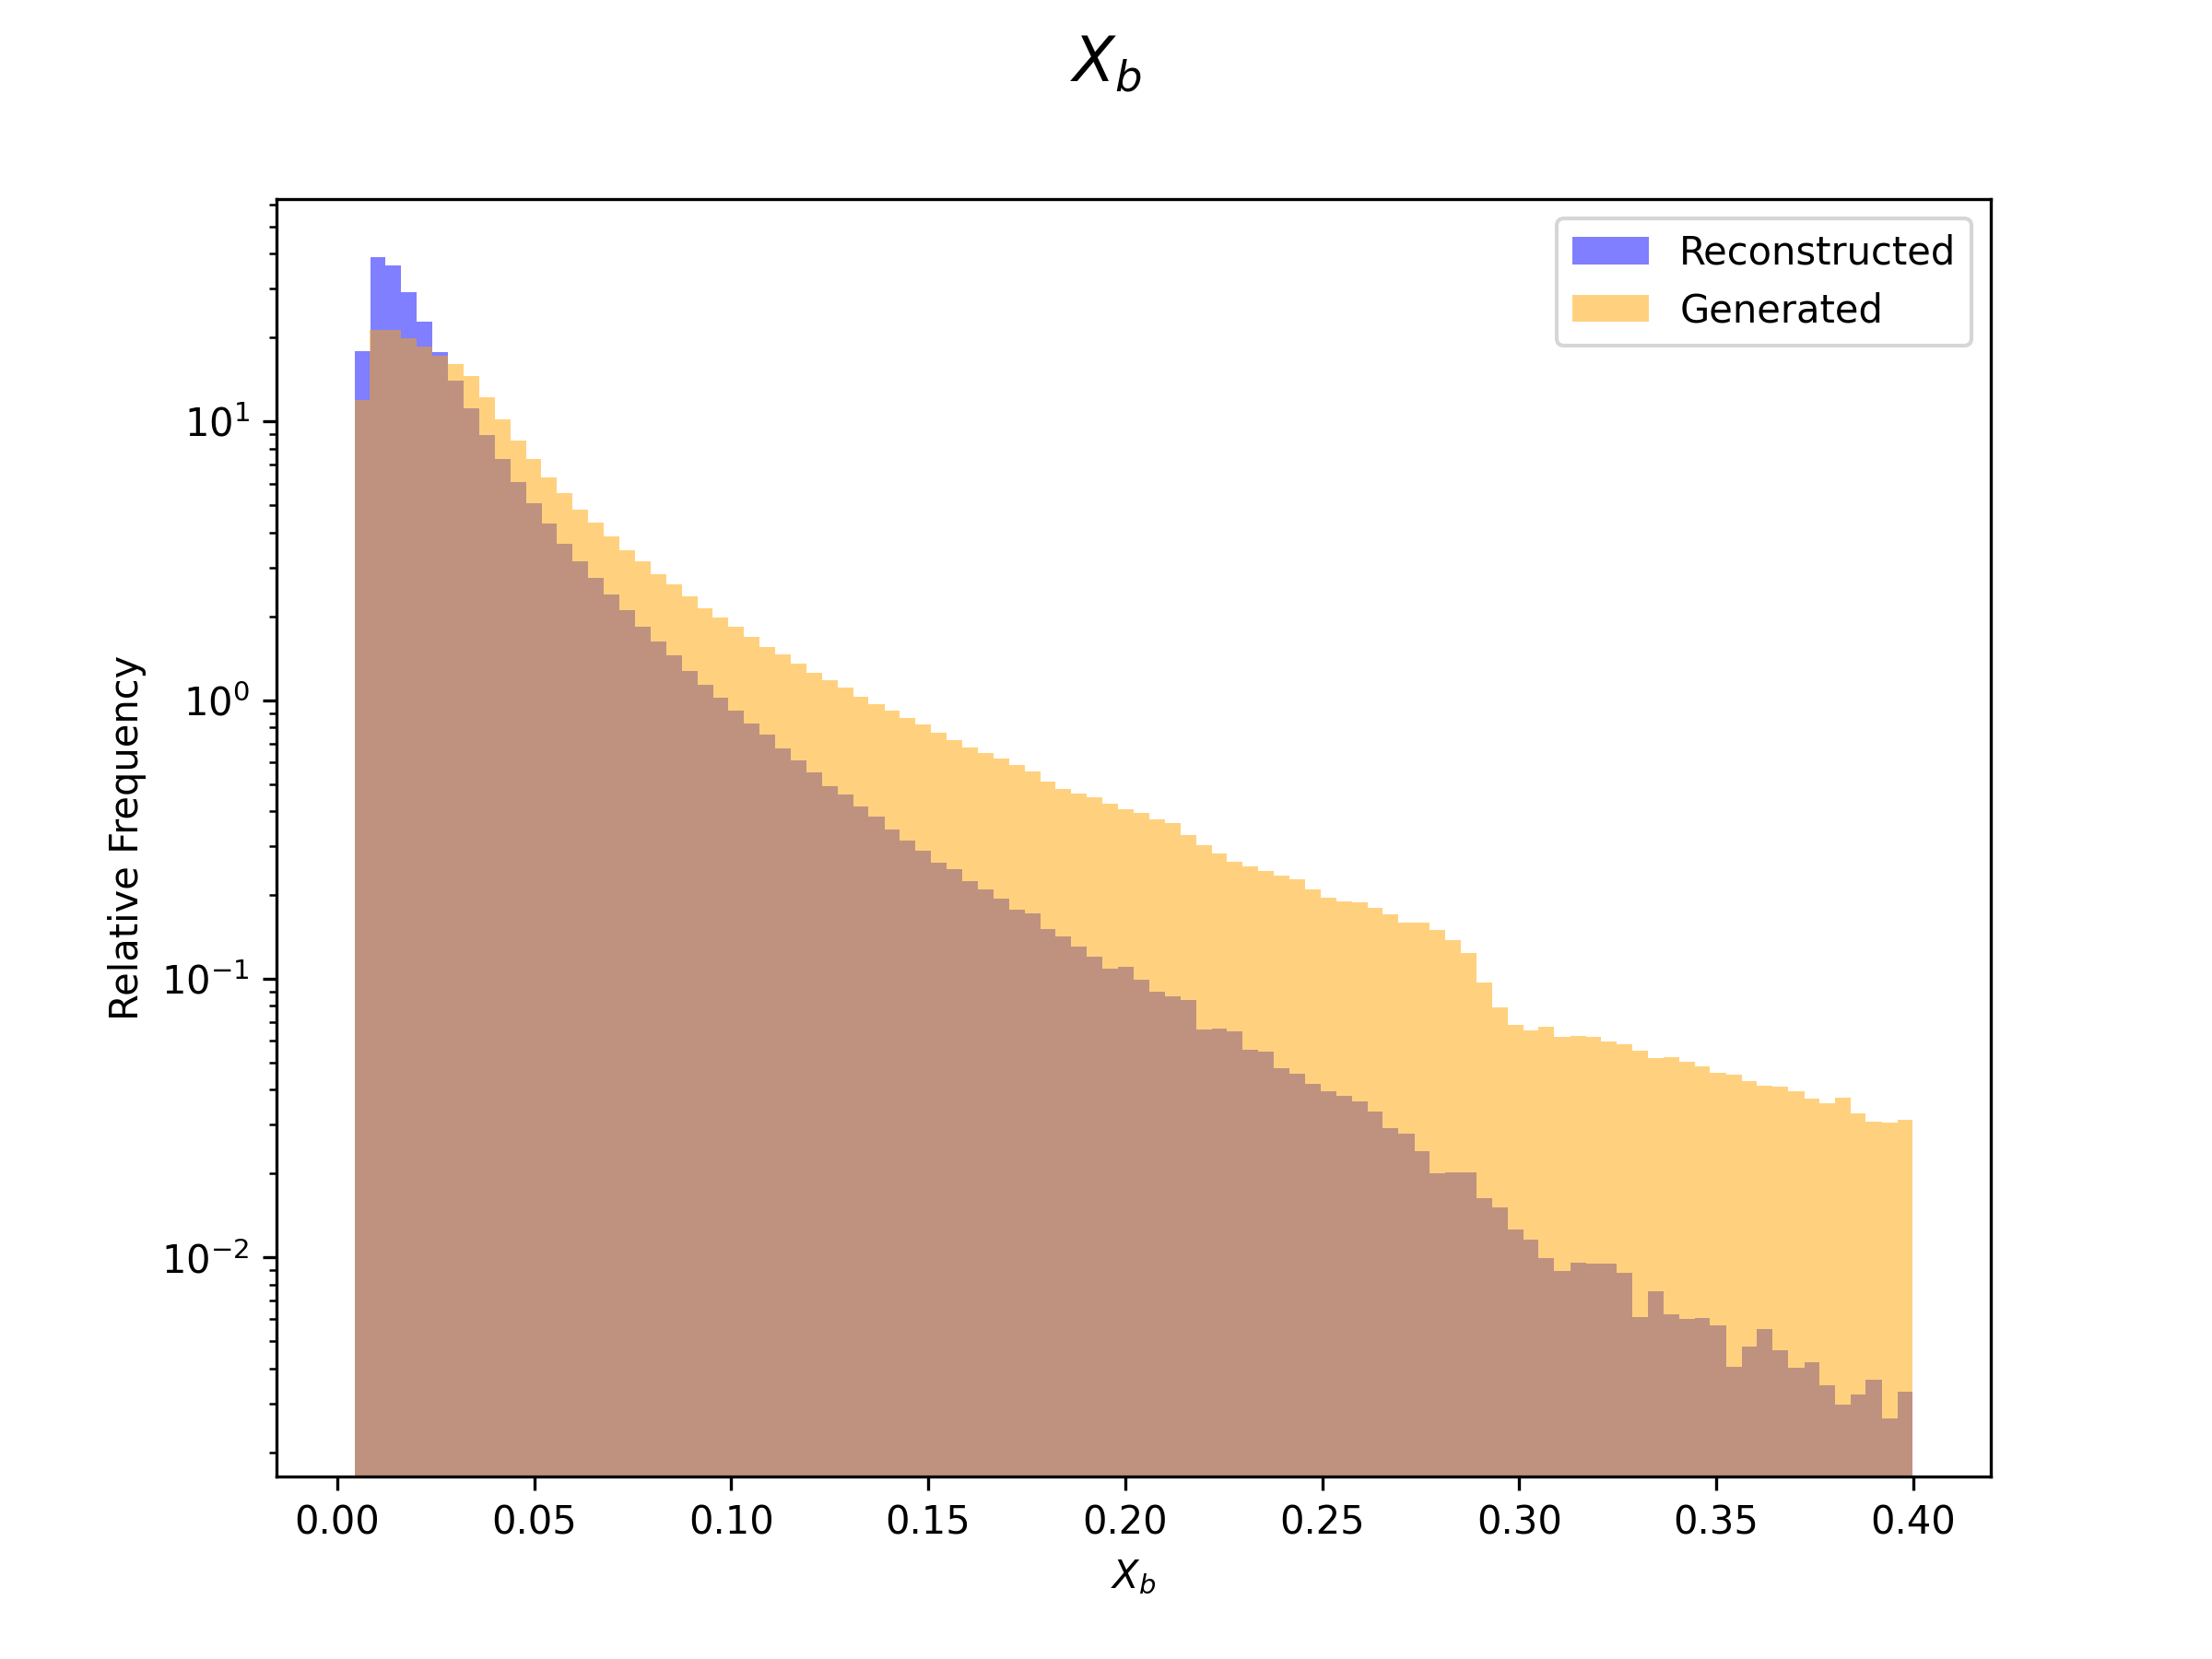
\includegraphics[width=\textwidth]{graphs/hadr_X_b.png}
        \caption{Histogram for $X_b$}
        \label{fig:had_X_b}
    \end{subfigure}
    \hfill
    \begin{subfigure}[b]{0.45\textwidth}
        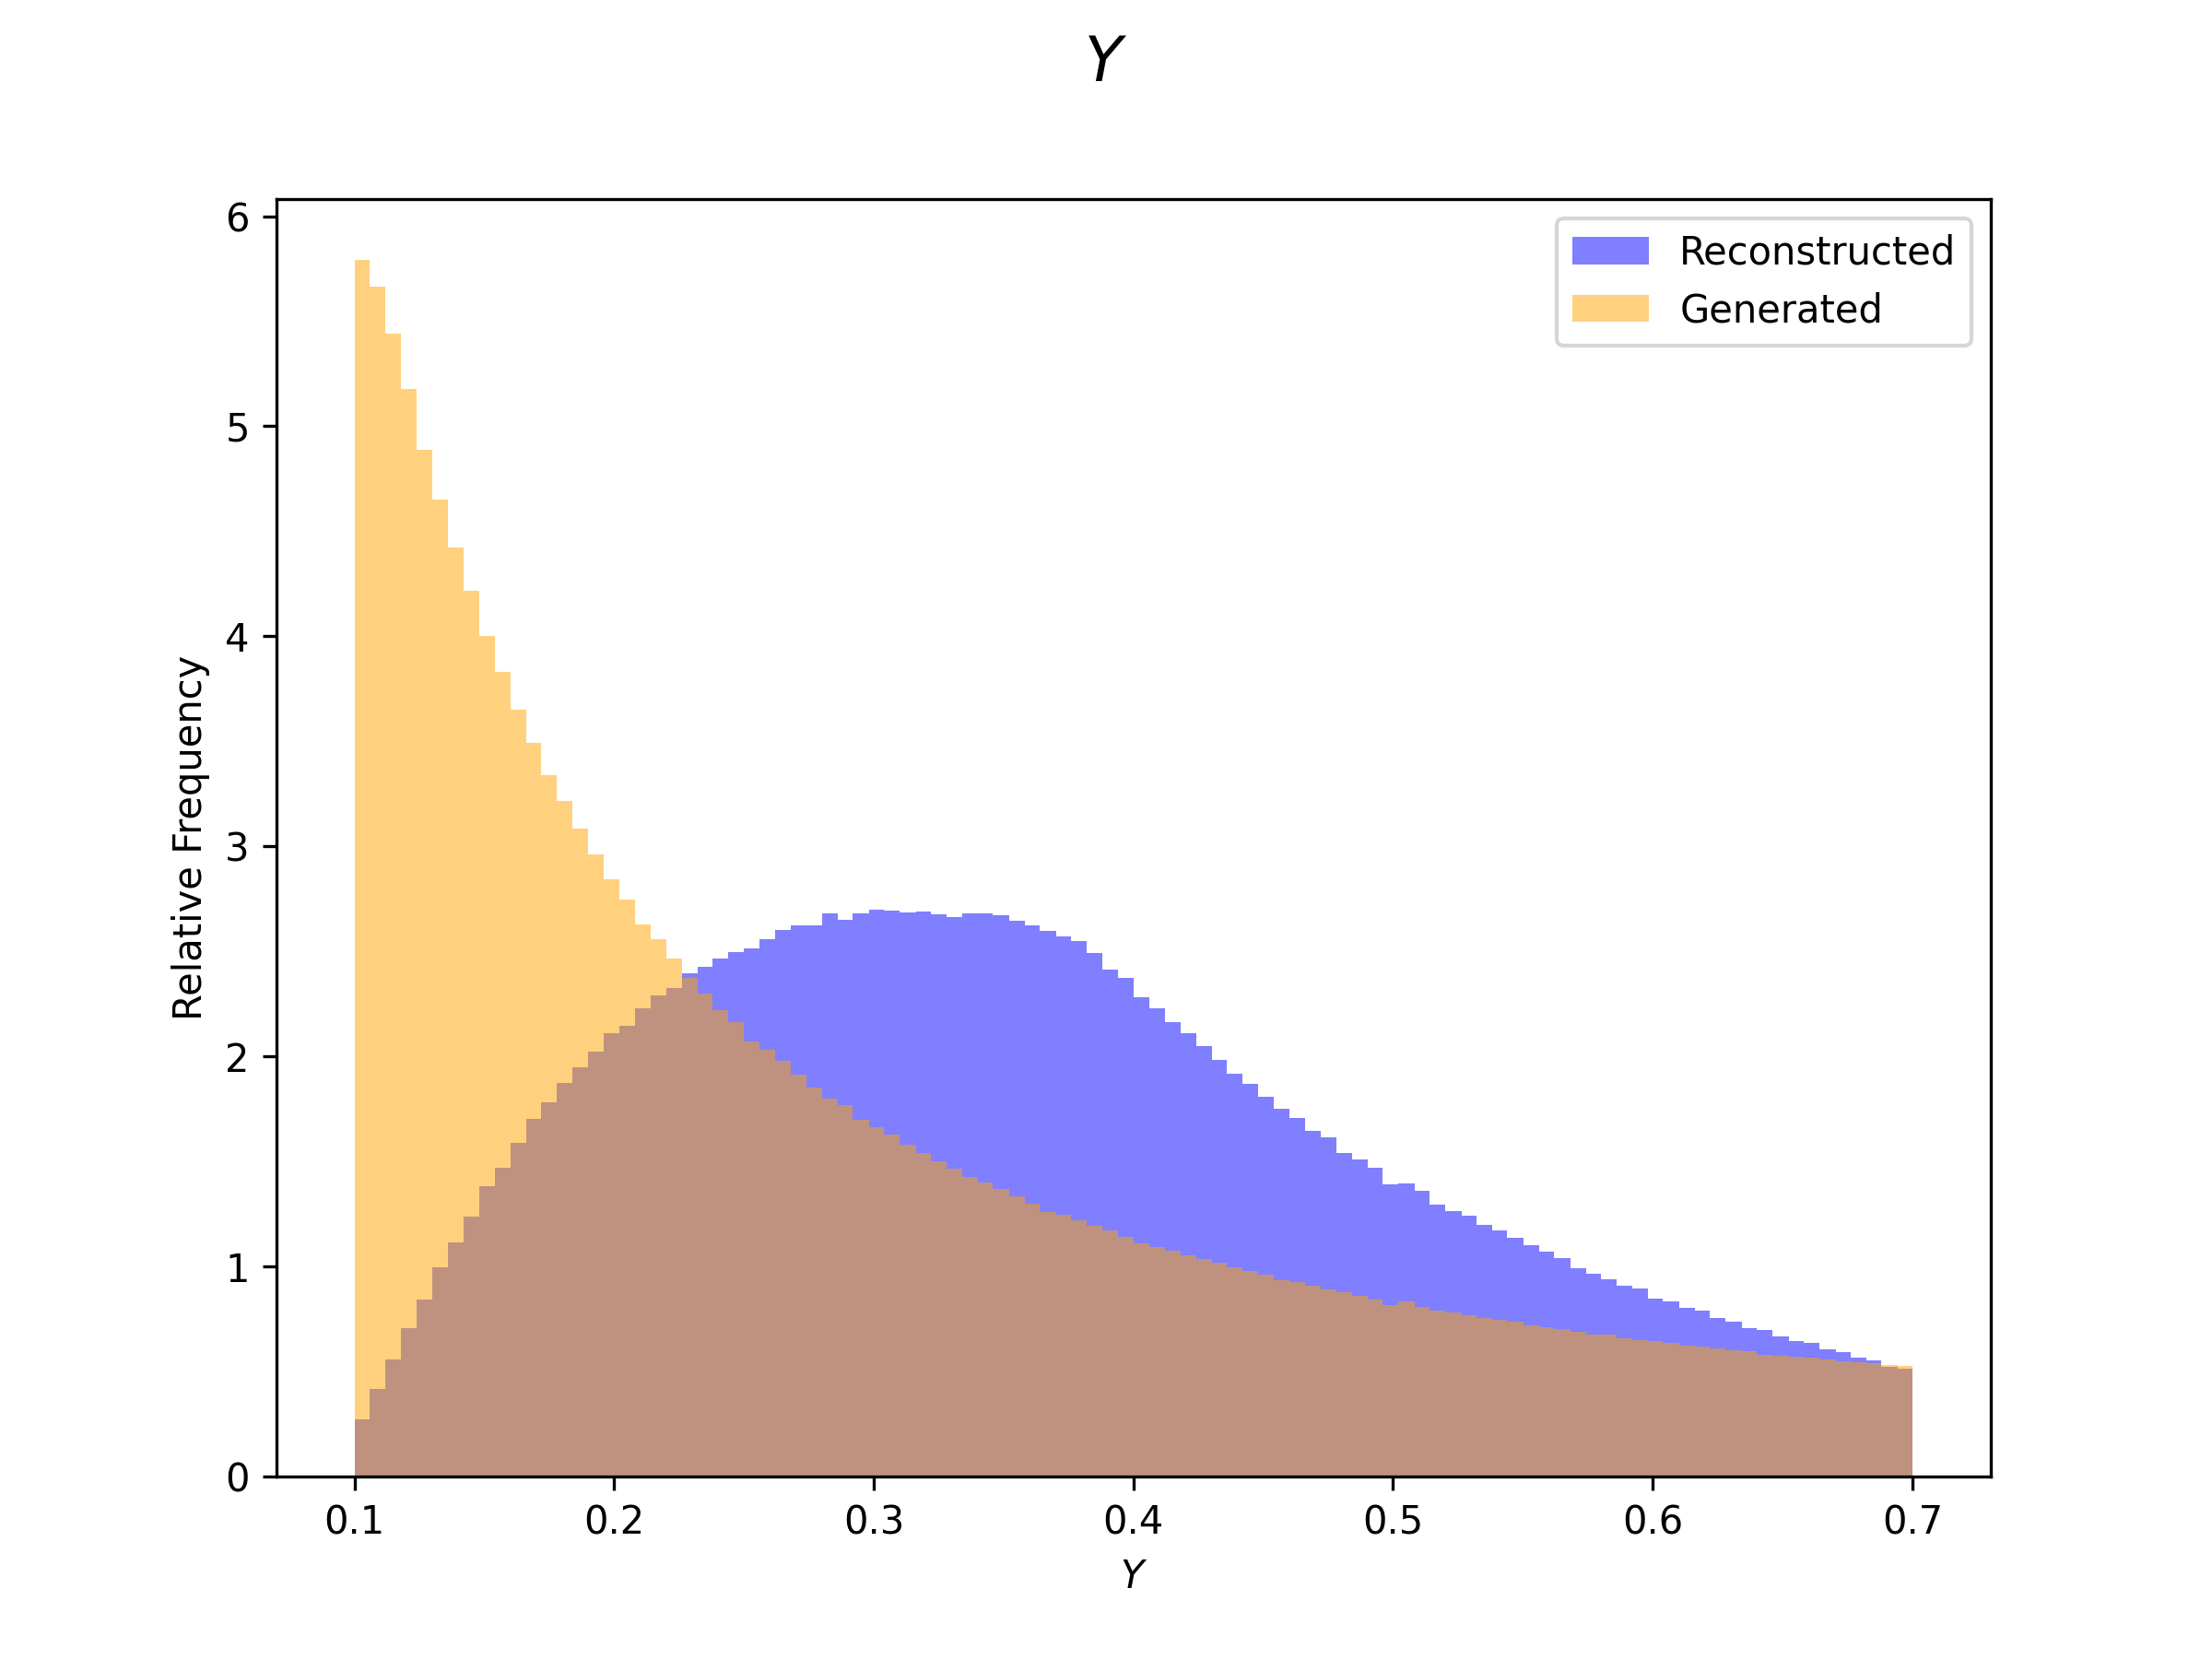
\includegraphics[width=\textwidth]{graphs/hadr_Y.png}
        \caption{Histogram for $Y$}
        \label{fig:had_Y}
    \end{subfigure}
    \caption{Histograms for $X_b$ and $Y$}
\end{figure}

\begin{figure}[H]
    \centering
    \begin{subfigure}[b]{0.45\textwidth}
        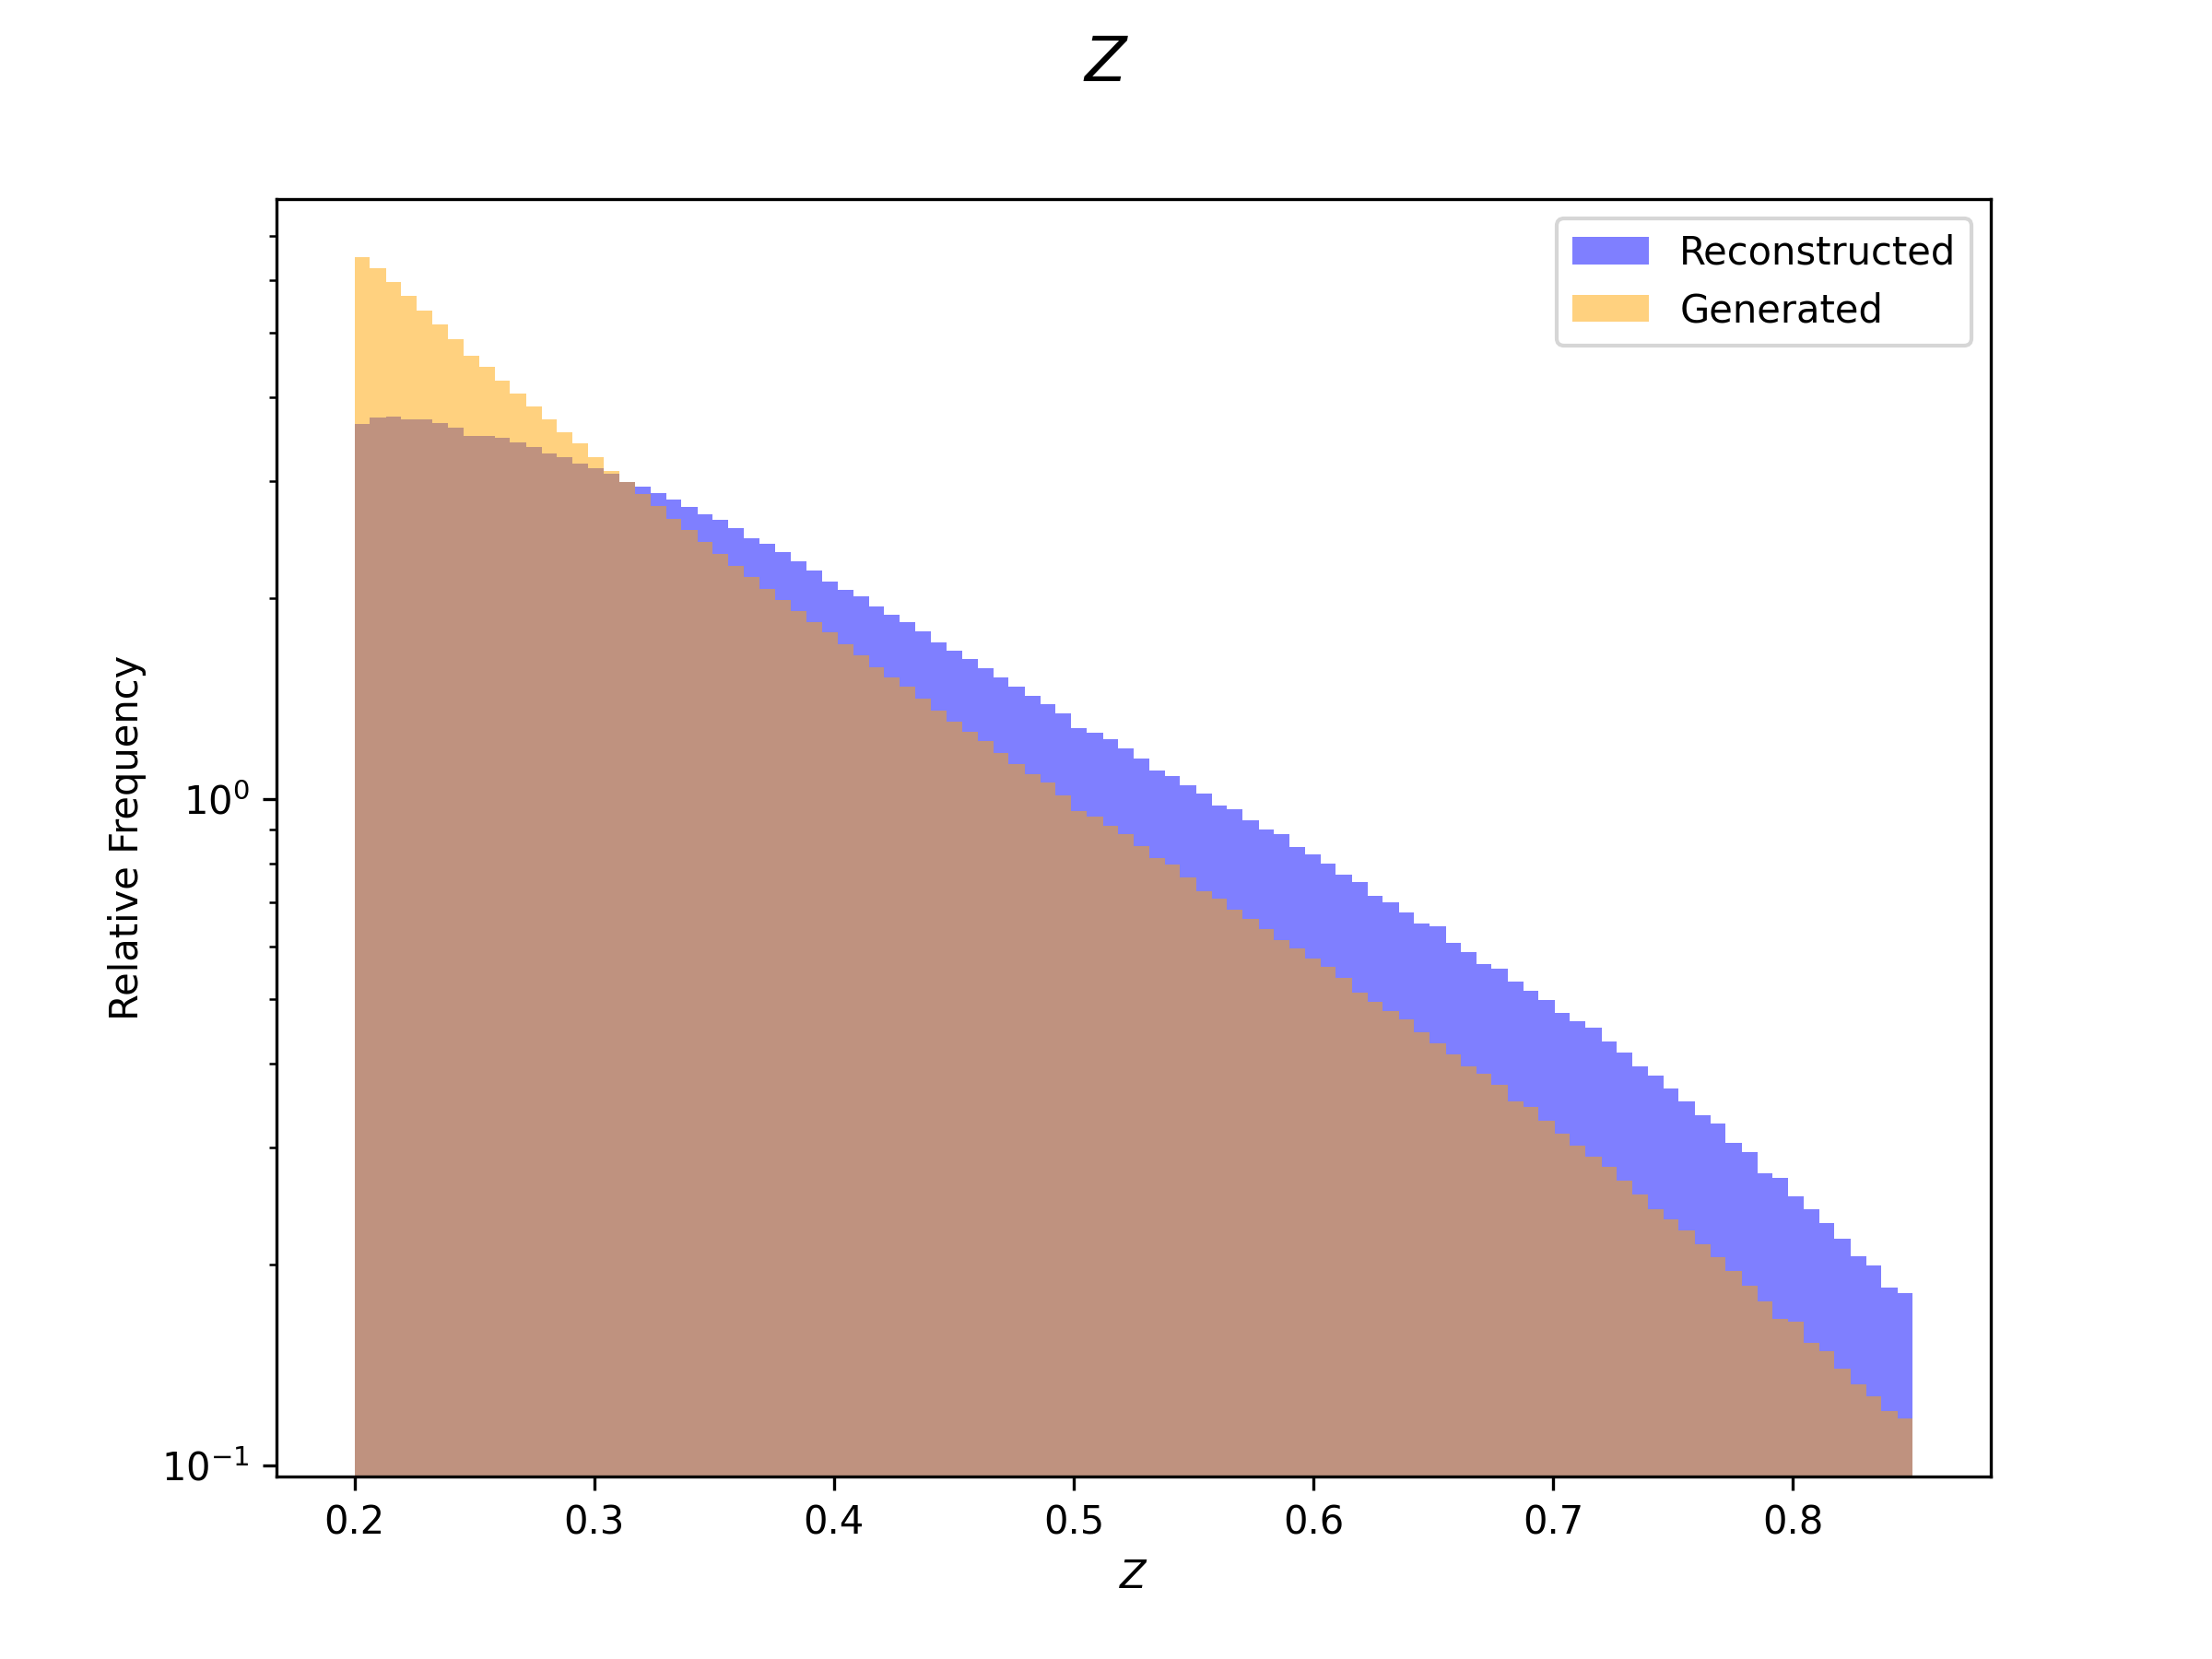
\includegraphics[width=\textwidth]{graphs/hadr_Z.png}
        \caption{Histogram for $Z$}
        \label{fig:had_Z}
    \end{subfigure}
    \hfill
    \begin{subfigure}[b]{0.45\textwidth}
        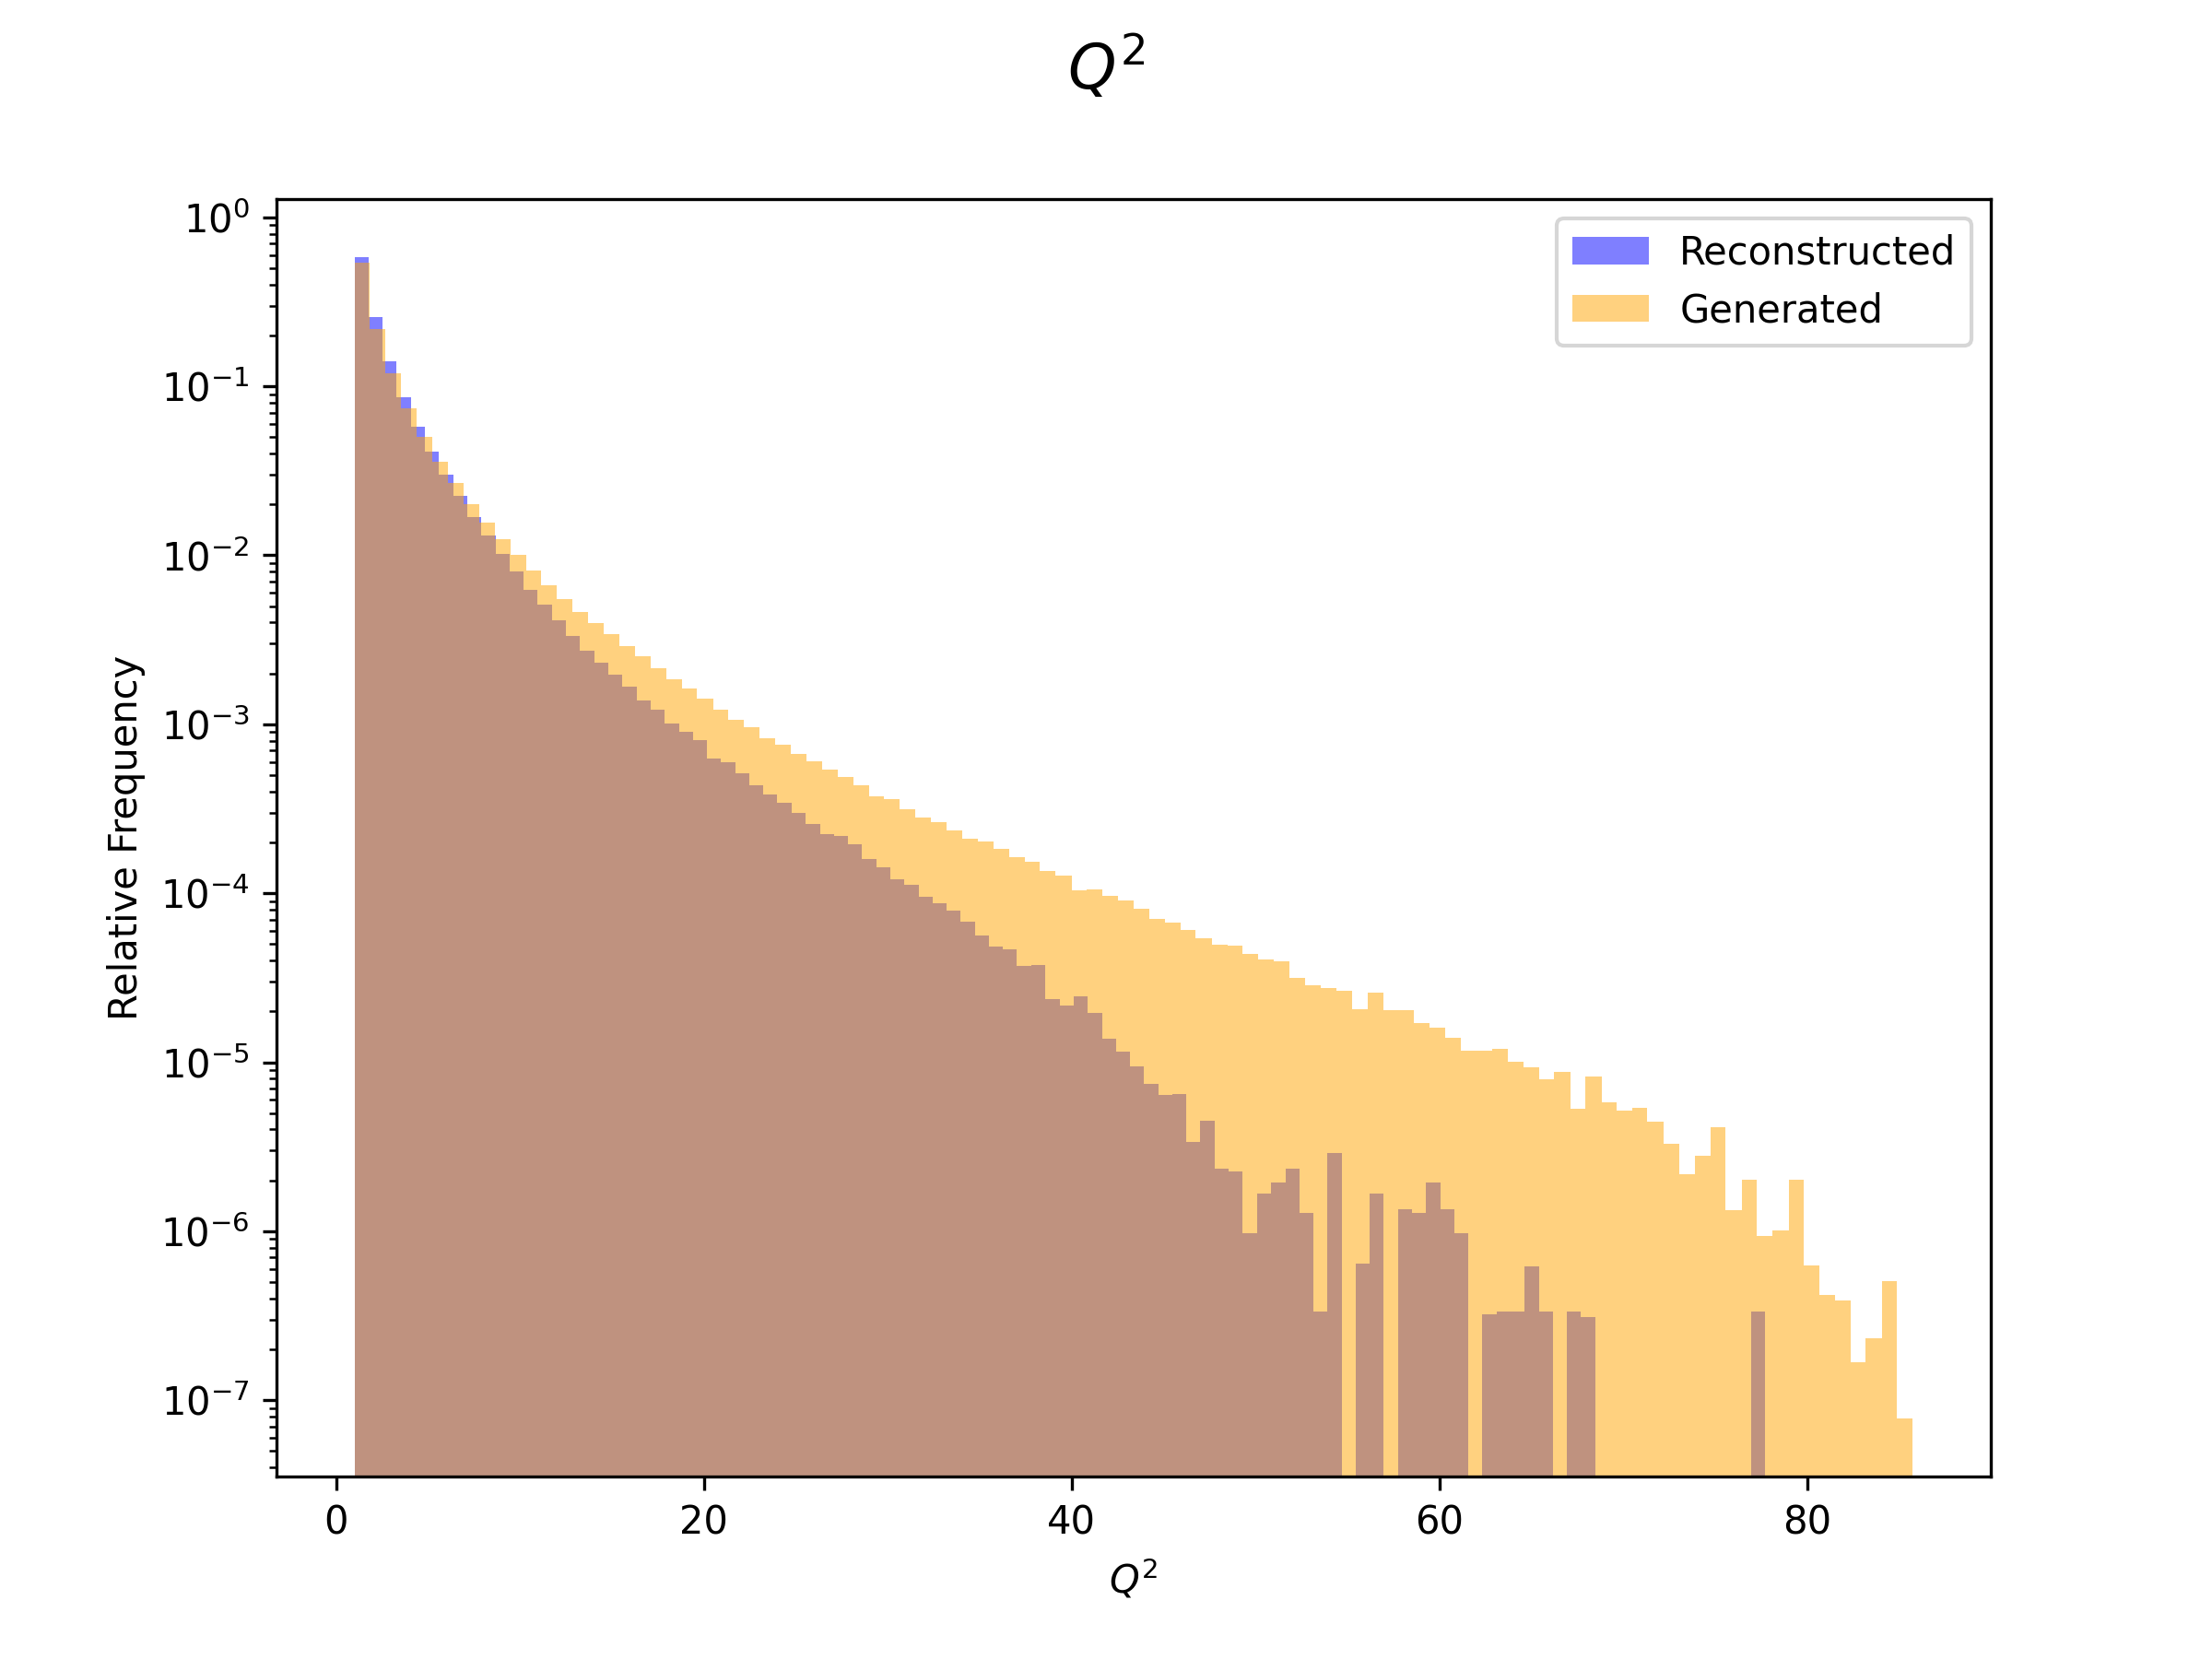
\includegraphics[width=\textwidth]{graphs/hadr_Q2.png}
        \caption{Histogram for $Q^2$}
        \label{fig:had_Q2}
    \end{subfigure}
    \caption{Histograms for $Z$ and $Q^2$}
\end{figure}

\begin{figure}[H]
    \centering
    \begin{subfigure}[b]{0.45\textwidth}
        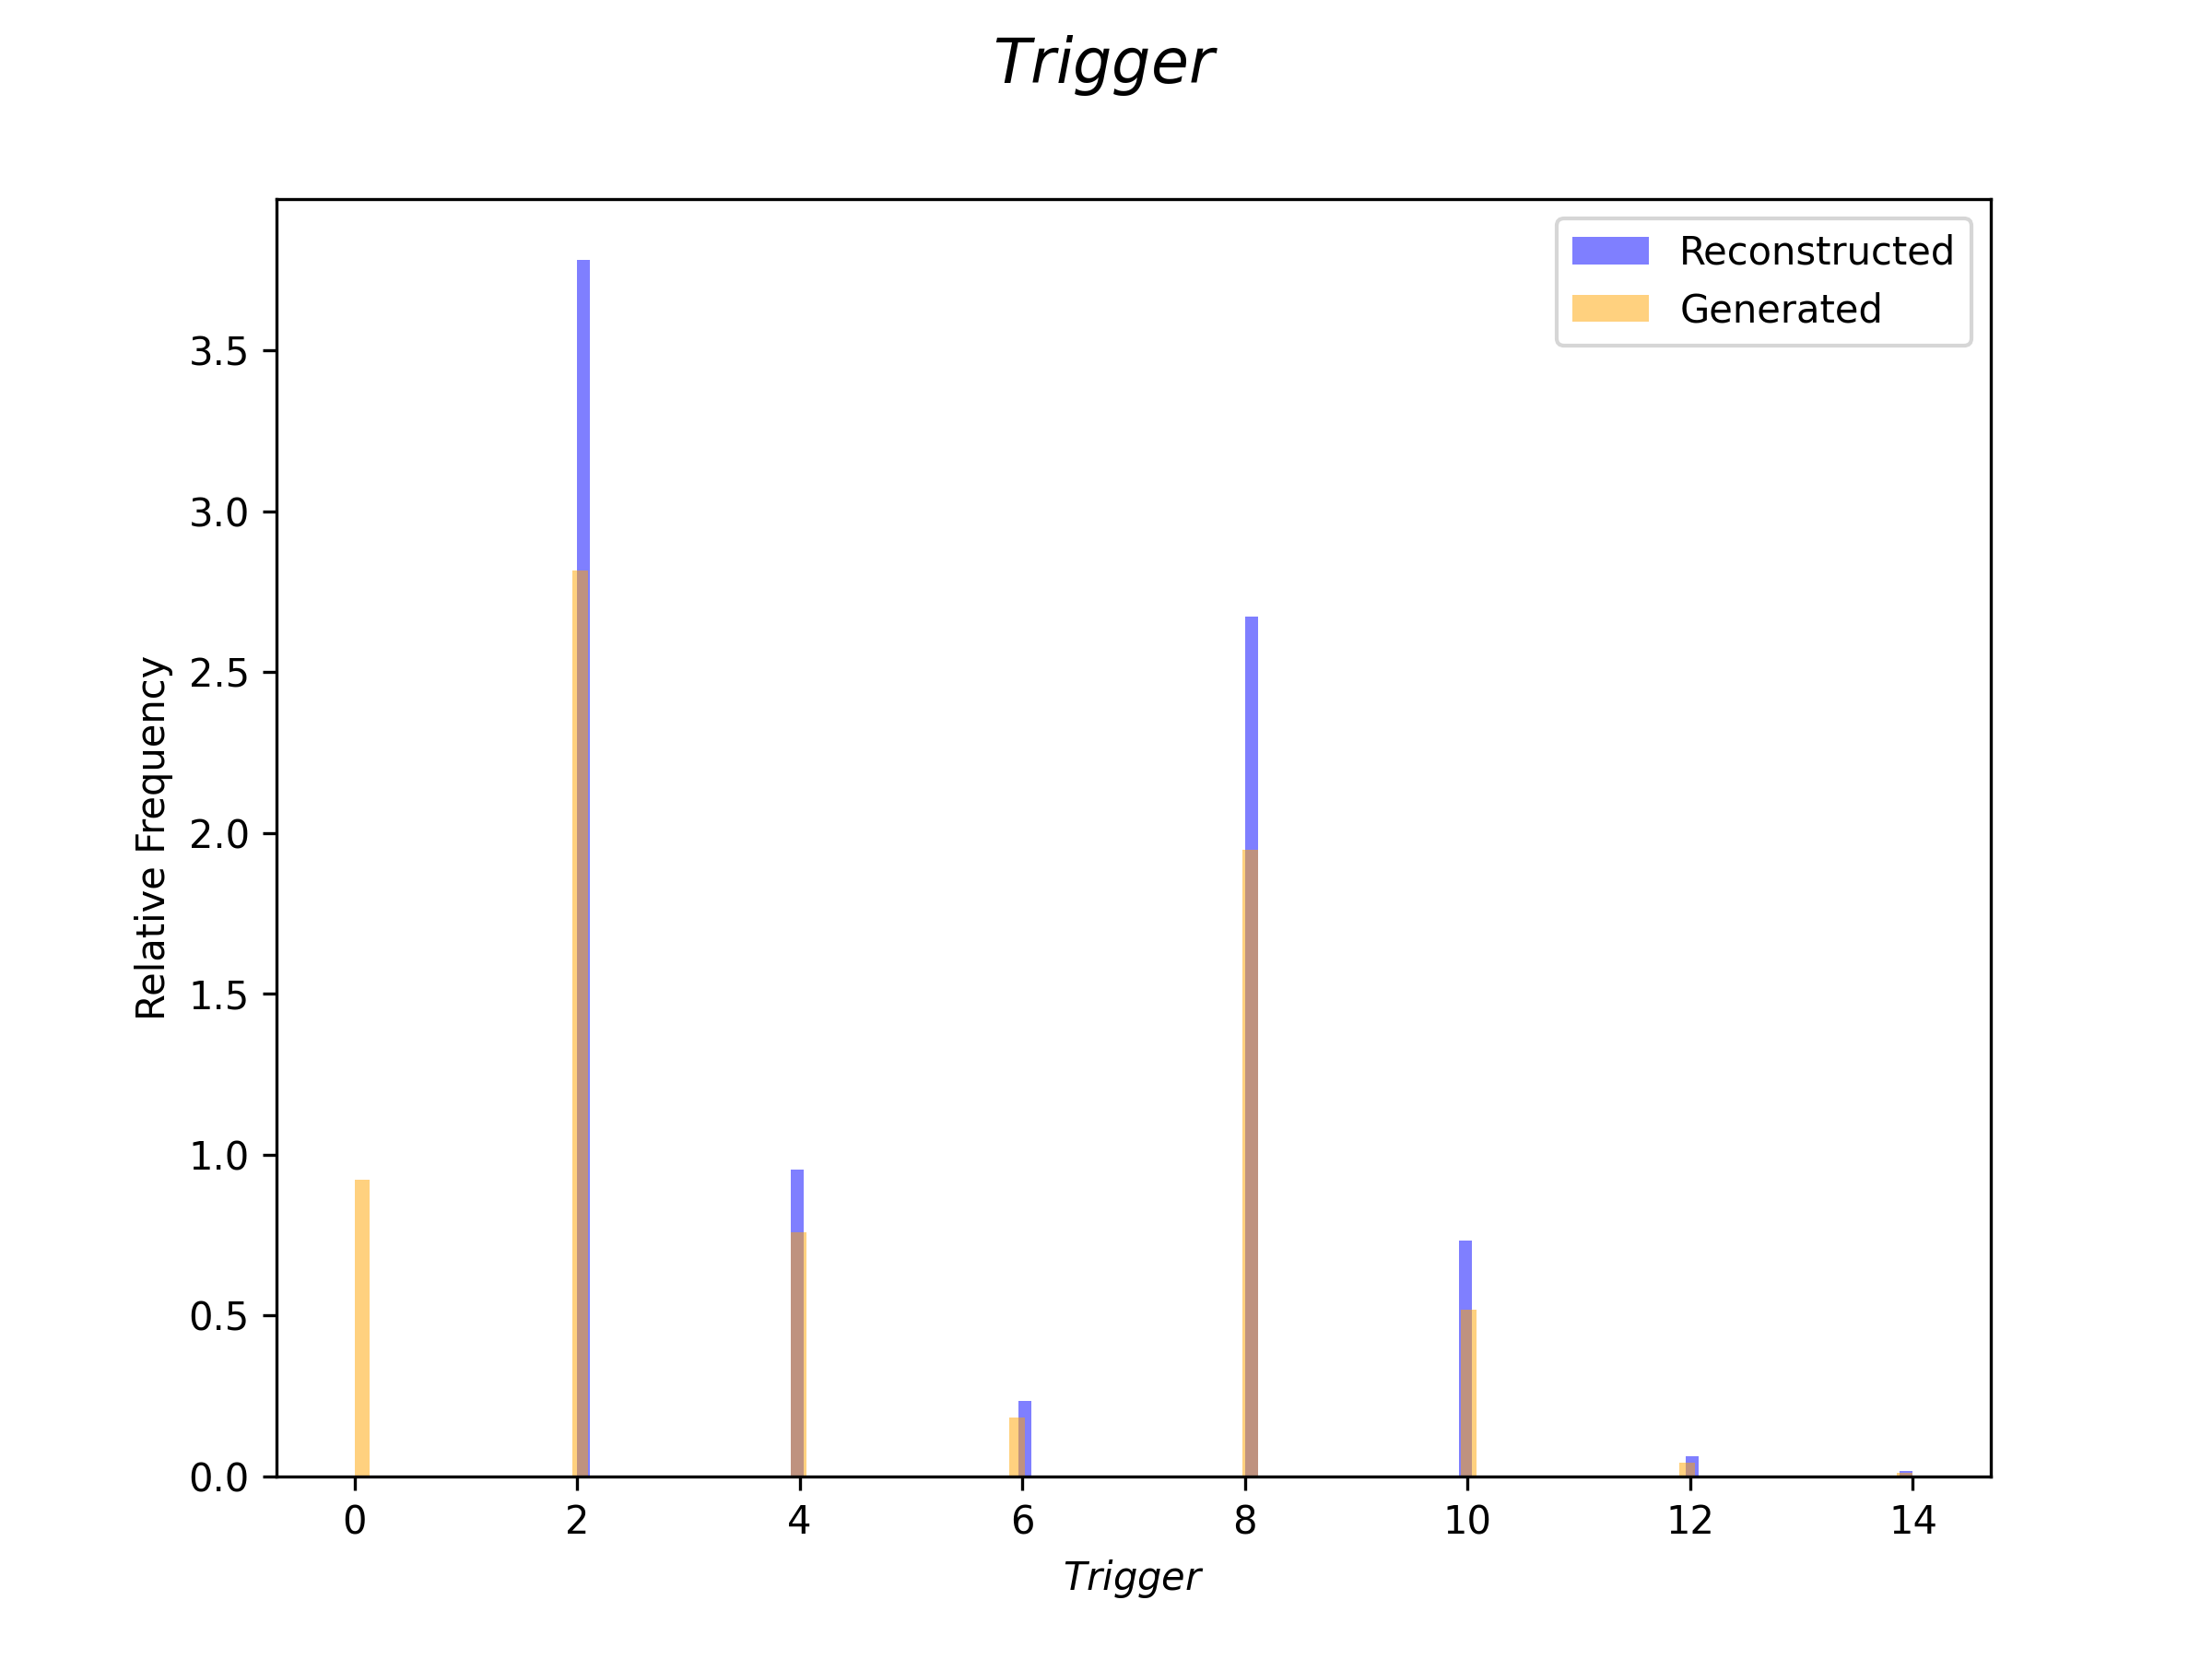
\includegraphics[width=\textwidth]{graphs/hadr_Trigger.png}
        \caption{Histogram for $Trig$}
        \label{fig:had_Trig}
    \end{subfigure}
    \hfill
    \begin{subfigure}[b]{0.45\textwidth}
        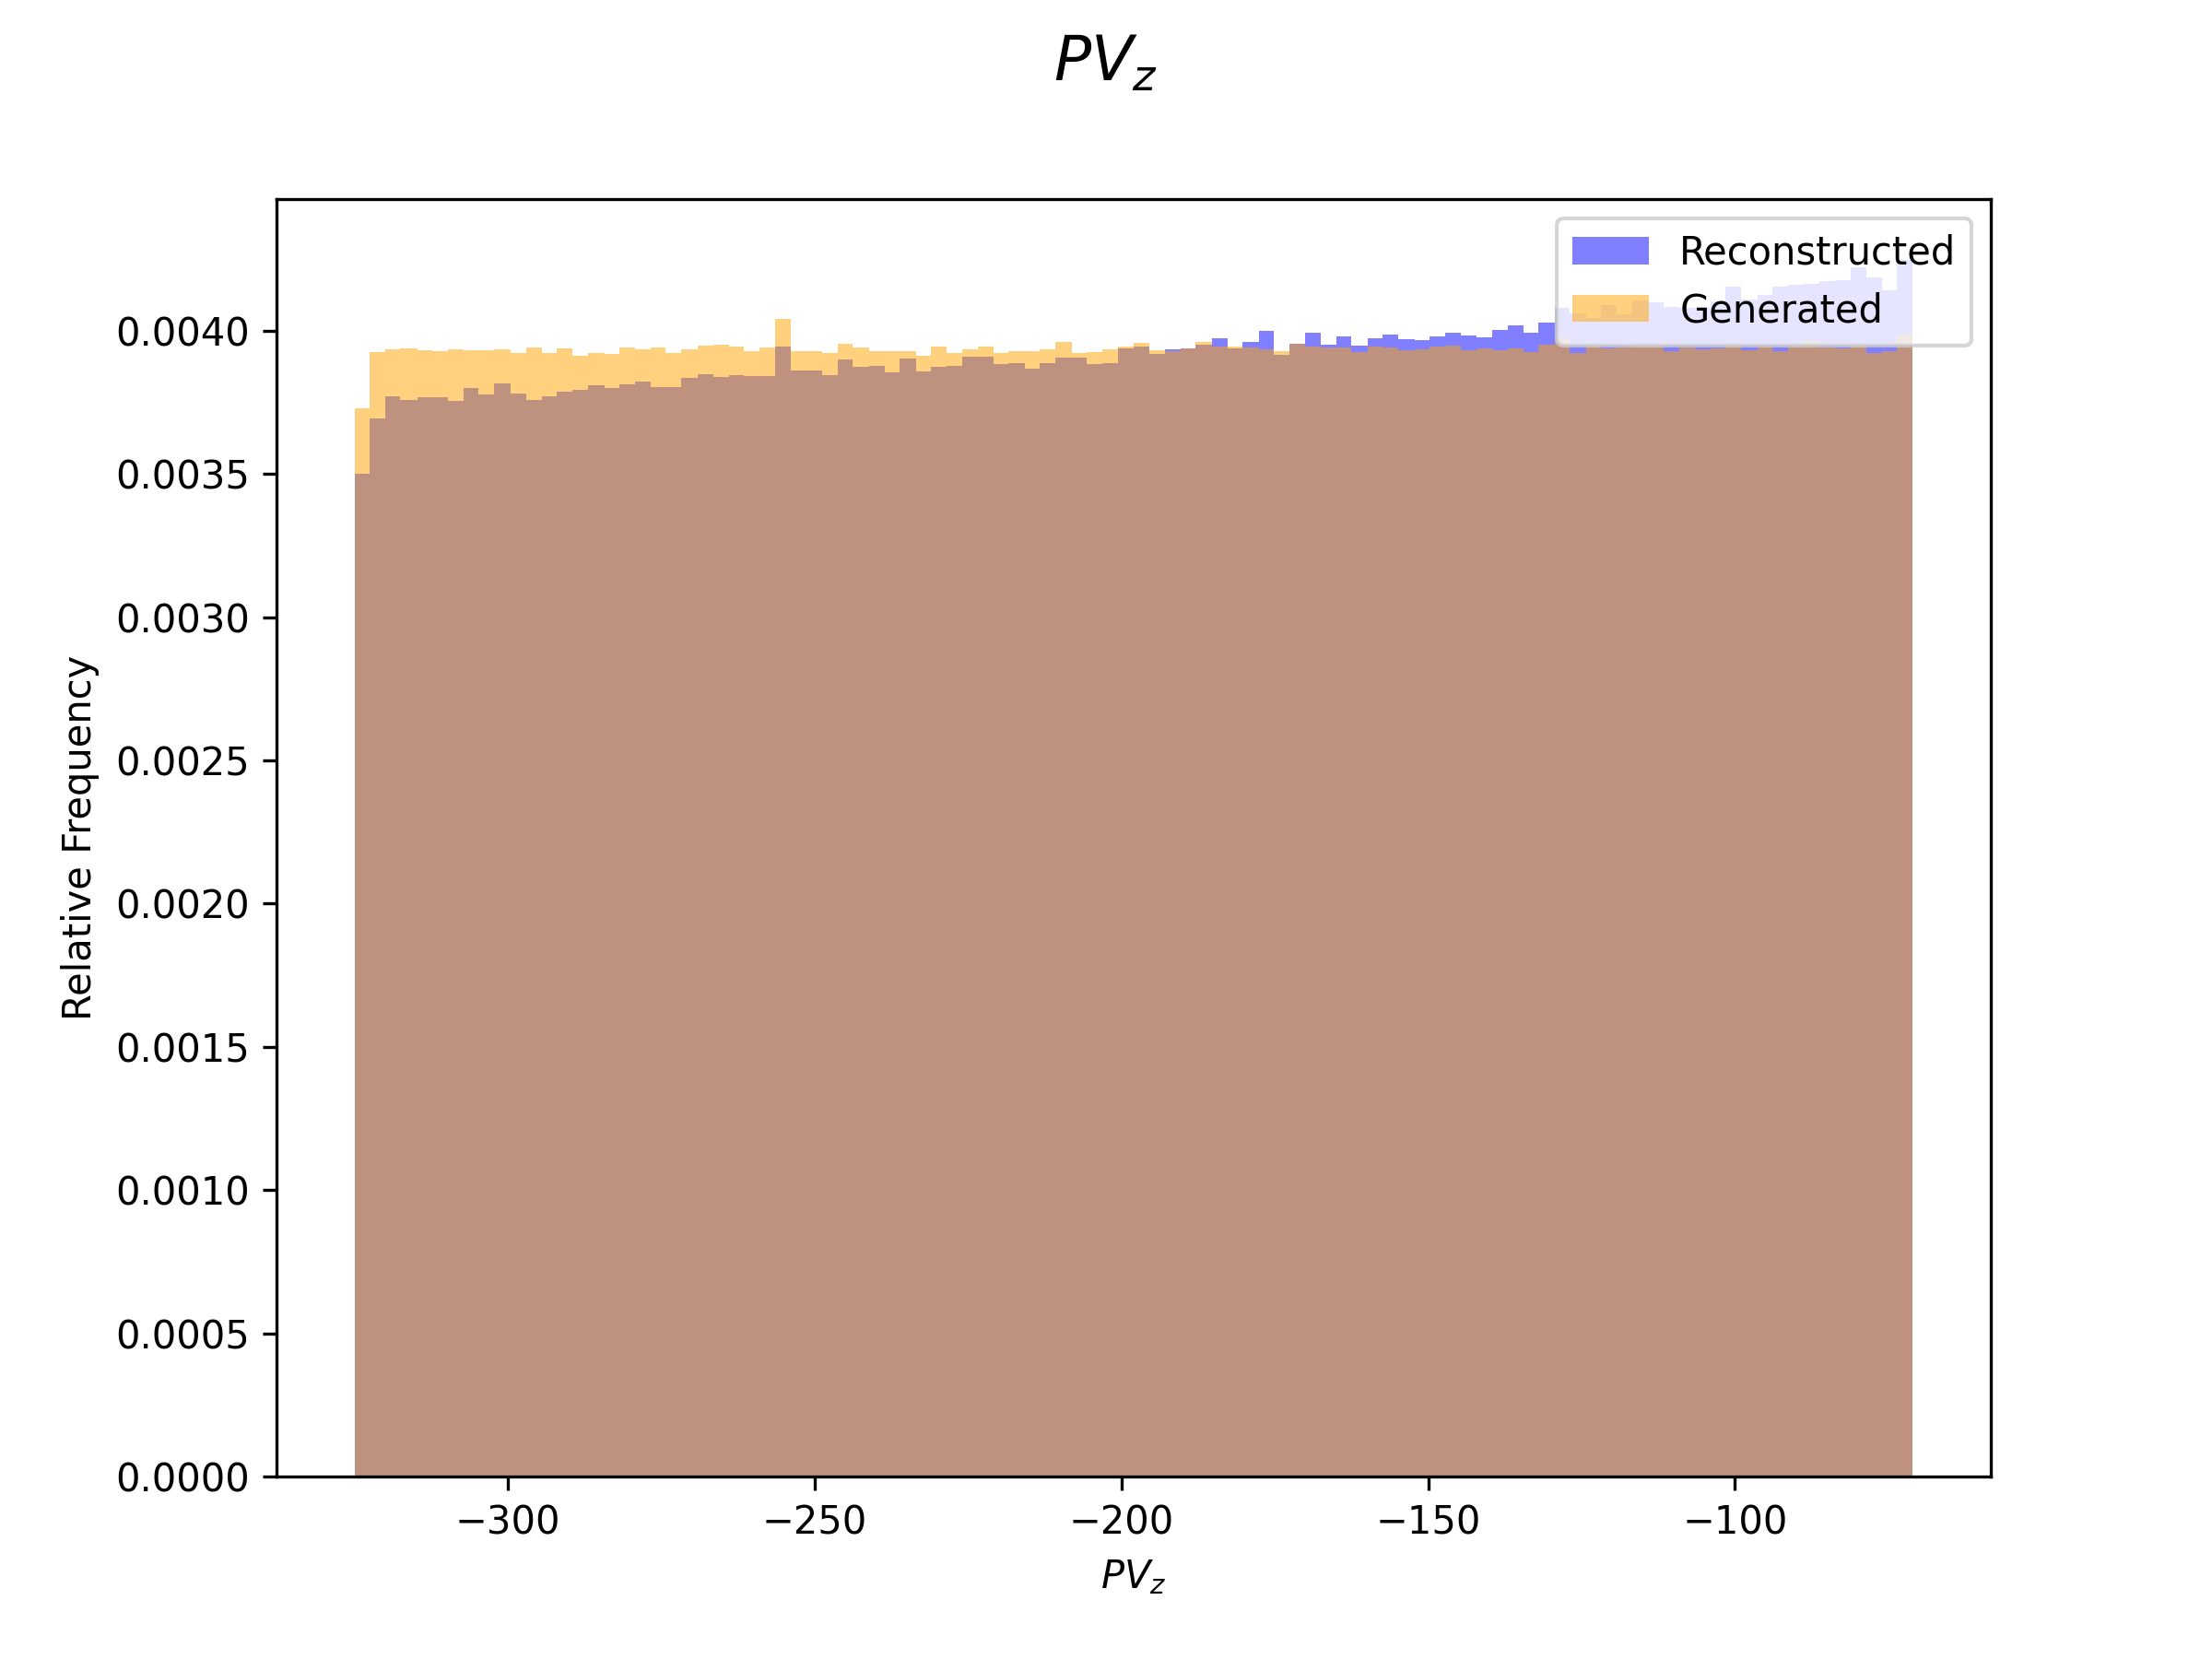
\includegraphics[width=\textwidth]{graphs/hadr_PV_z.png}
        \caption{Histogram for $PV_z$}
        \label{fig:had_PV_z}
    \end{subfigure}
    \caption{Histograms for $Trig$ and $PV_z$}
\end{figure}


\begin{figure}[H]
    \centering
    \begin{subfigure}[b]{0.45\textwidth}
        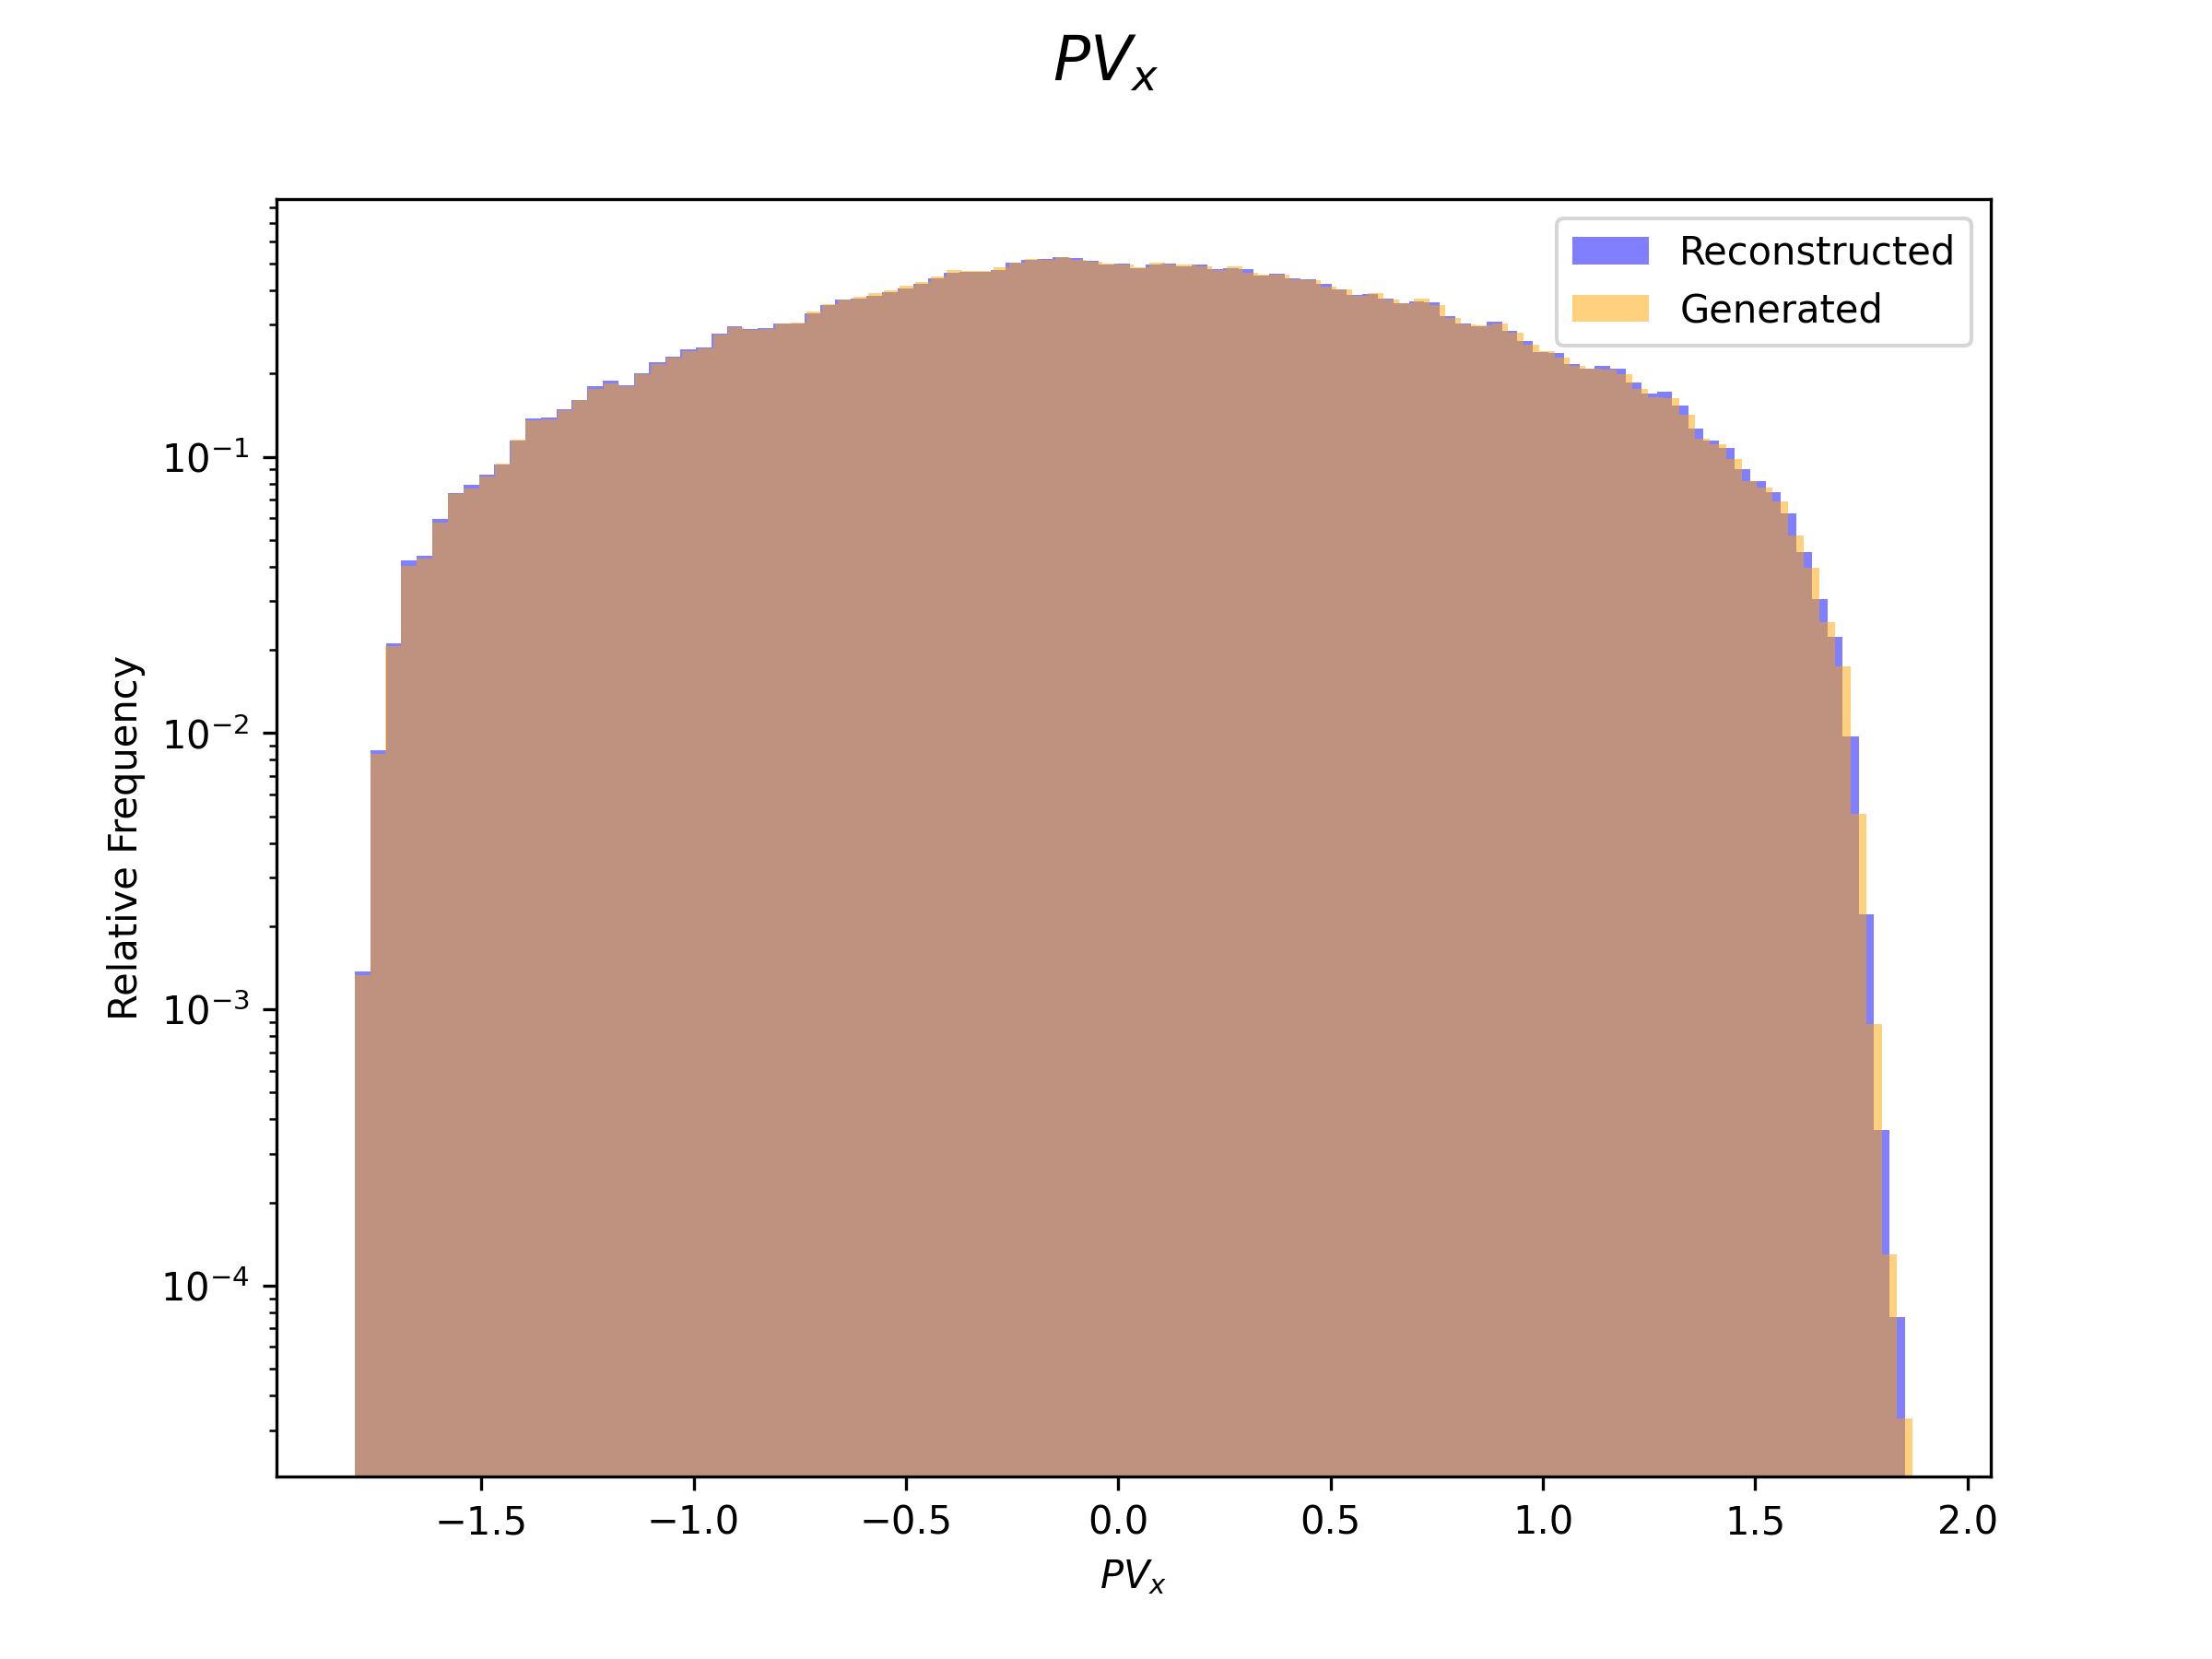
\includegraphics[width=\textwidth]{graphs/hadr_PV_x.png}
        \caption{Histogram for $PV_x$}
        \label{fig:had_PV_x}
    \end{subfigure}
    \hfill
    \begin{subfigure}[b]{0.45\textwidth}
        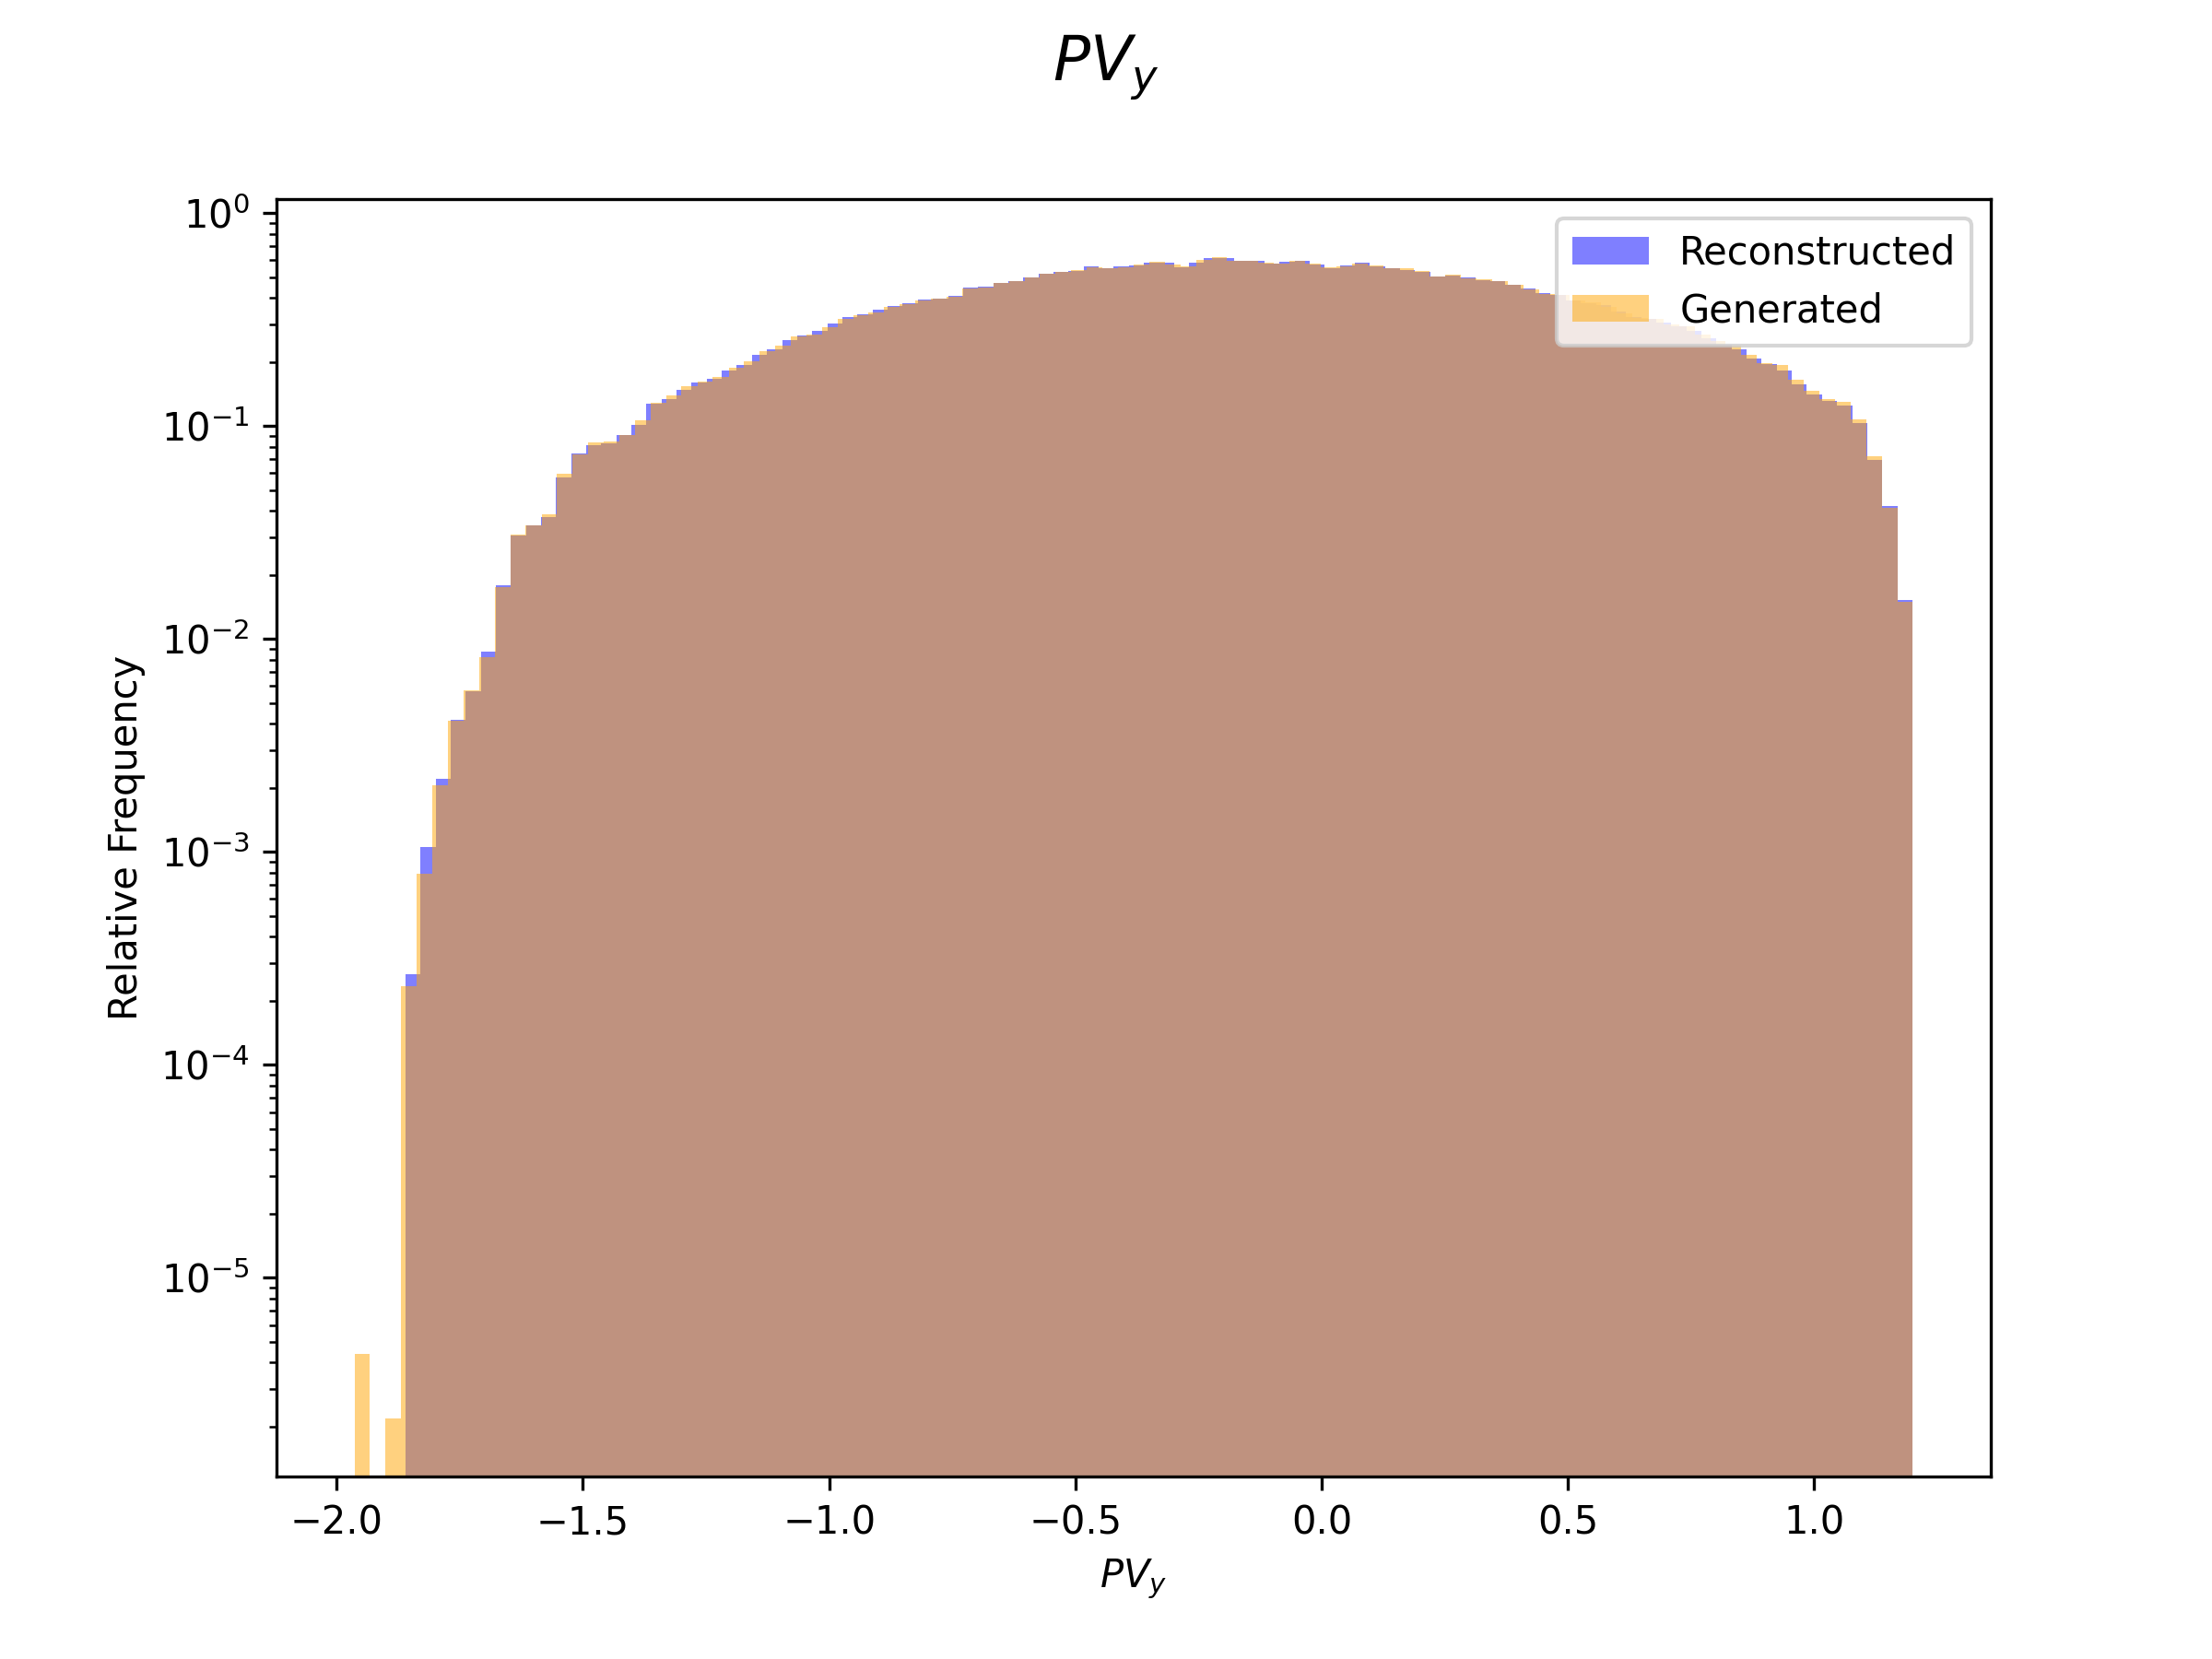
\includegraphics[width=\textwidth]{graphs/hadr_PV_y.png}
        \caption{Histogram for $PV_y$}
        \label{fig:had_PV_y}
    \end{subfigure}
    \caption{Histograms for $PV_x$ and $PV_y$}
\end{figure}

\begin{figure}[H]
    \centering
    \begin{subfigure}[b]{0.45\textwidth}
        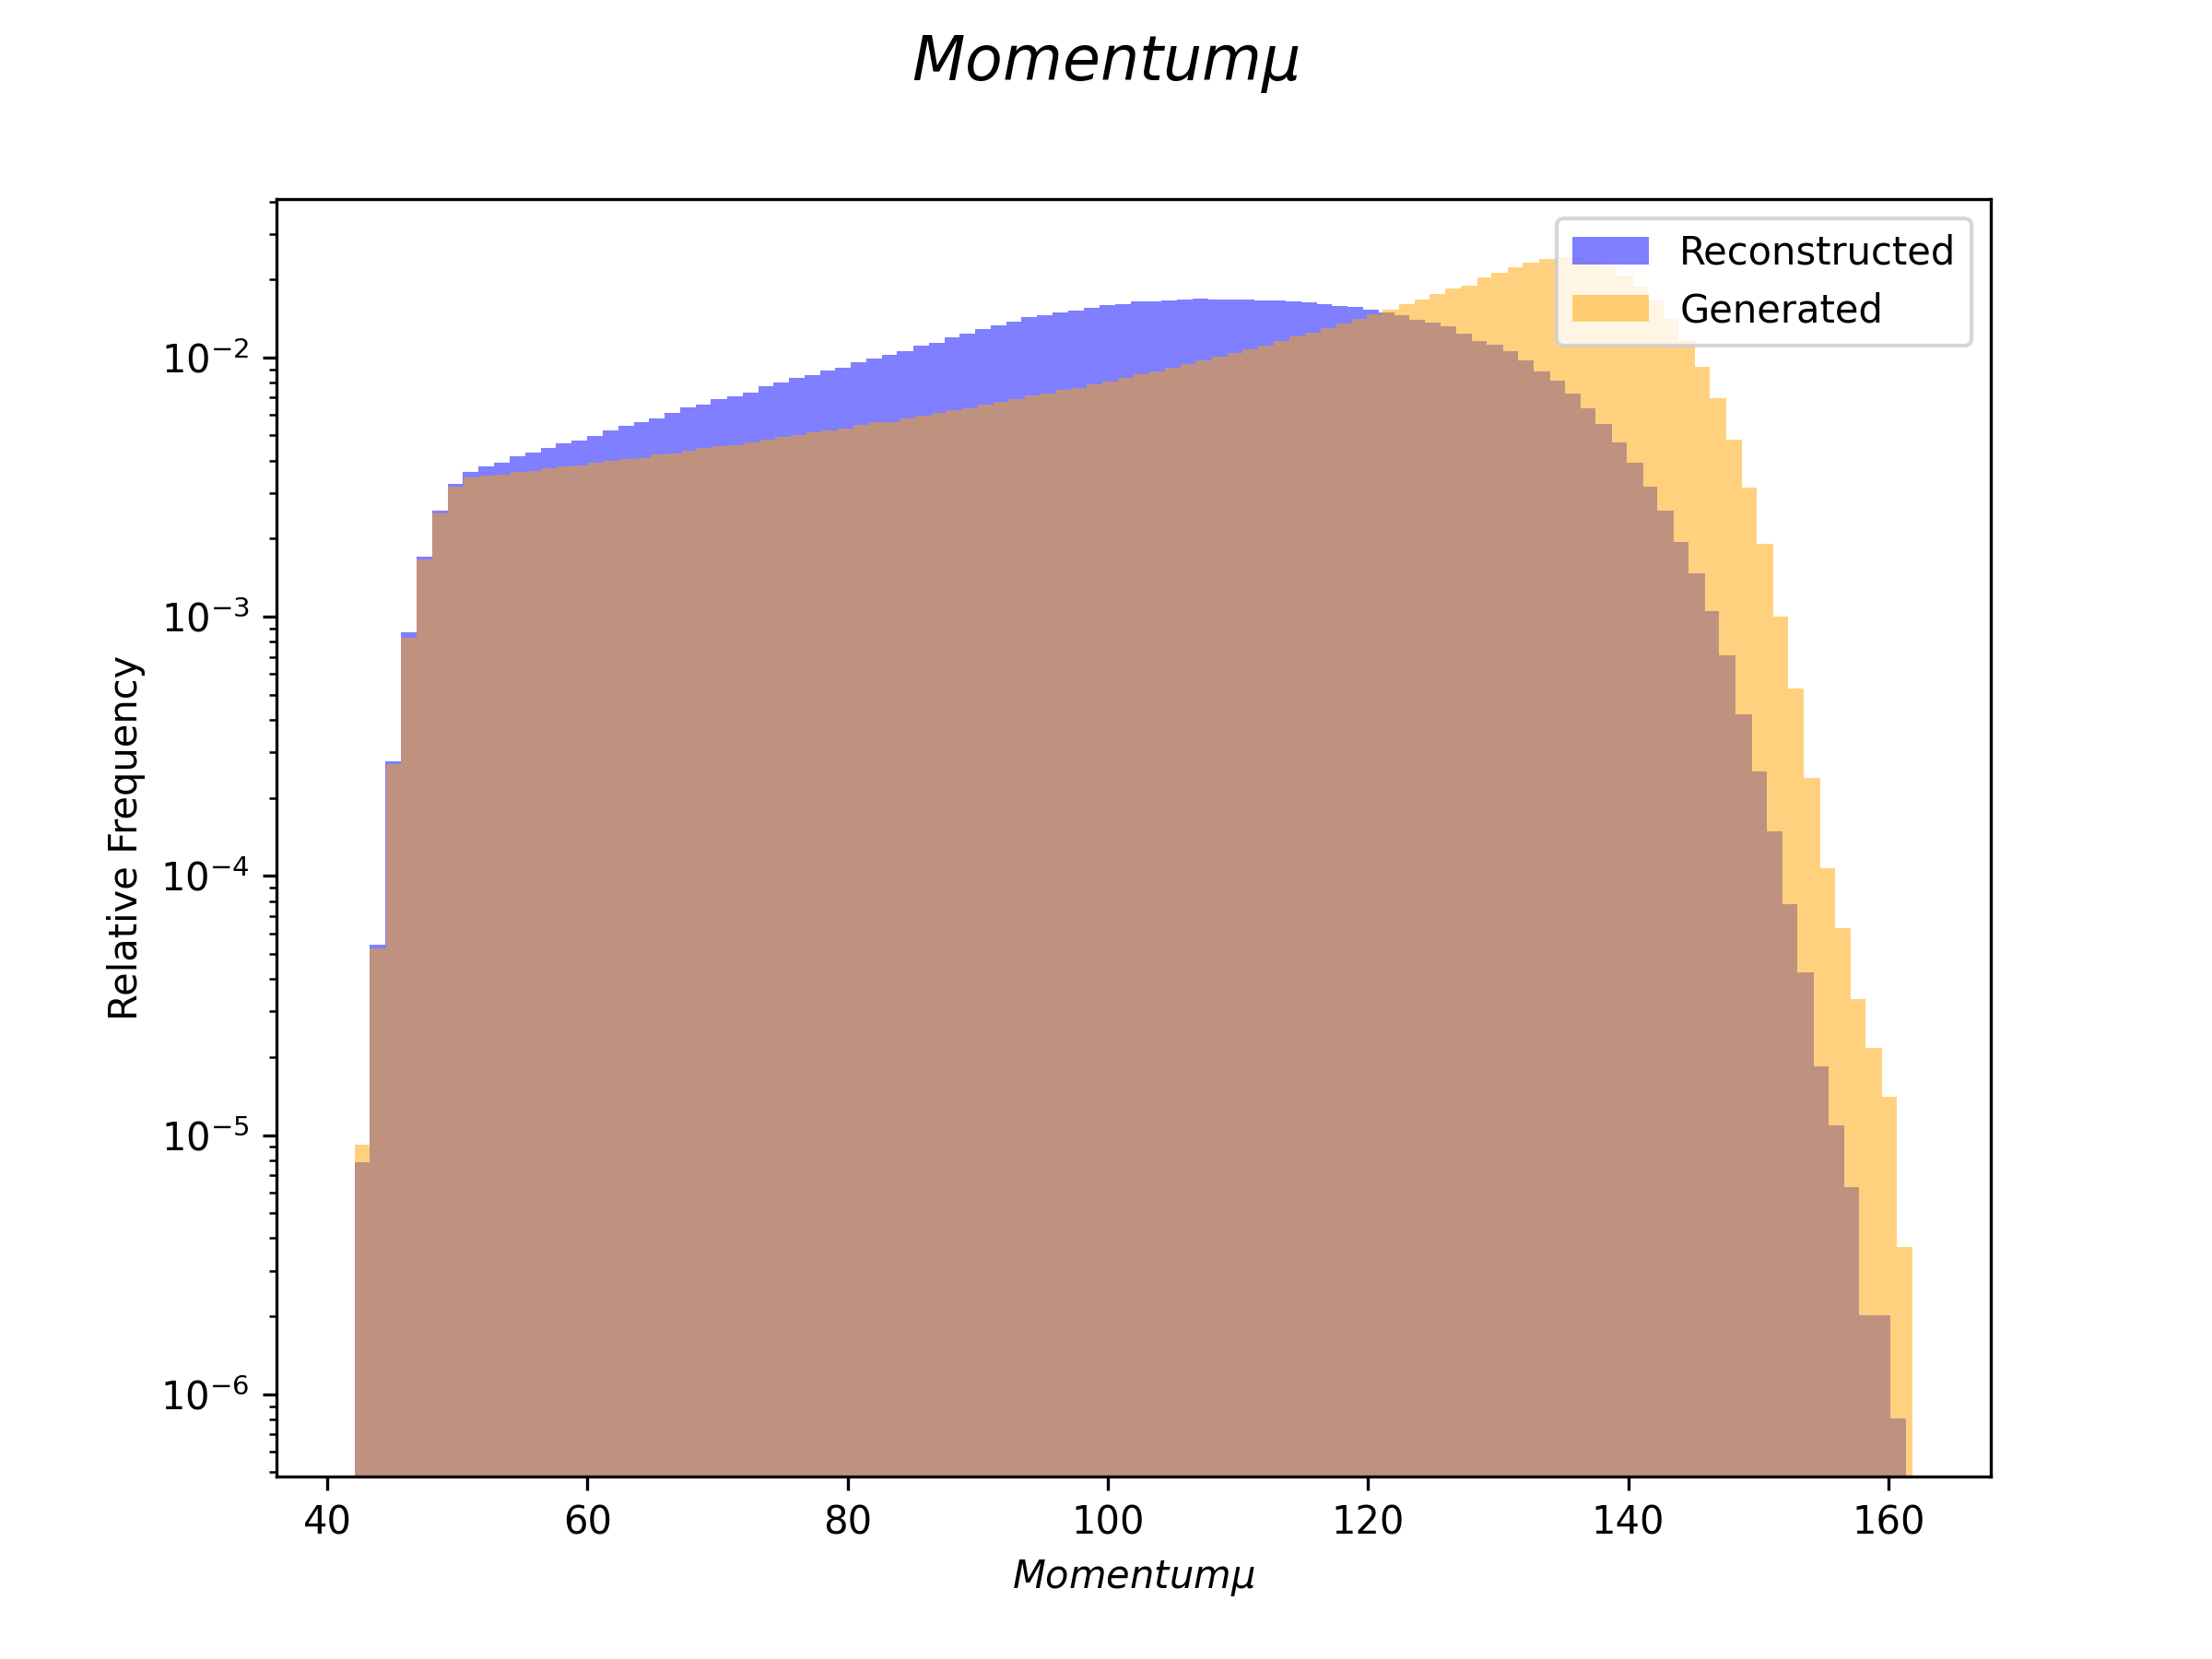
\includegraphics[width=\textwidth]{graphs/hadr_Momentum_mu.png}
        \caption{Histogram for $Mom_{mu}$}
        \label{fig:had_Momentum_mu}
    \end{subfigure}
    \hfill
    \begin{subfigure}[b]{0.45\textwidth}
        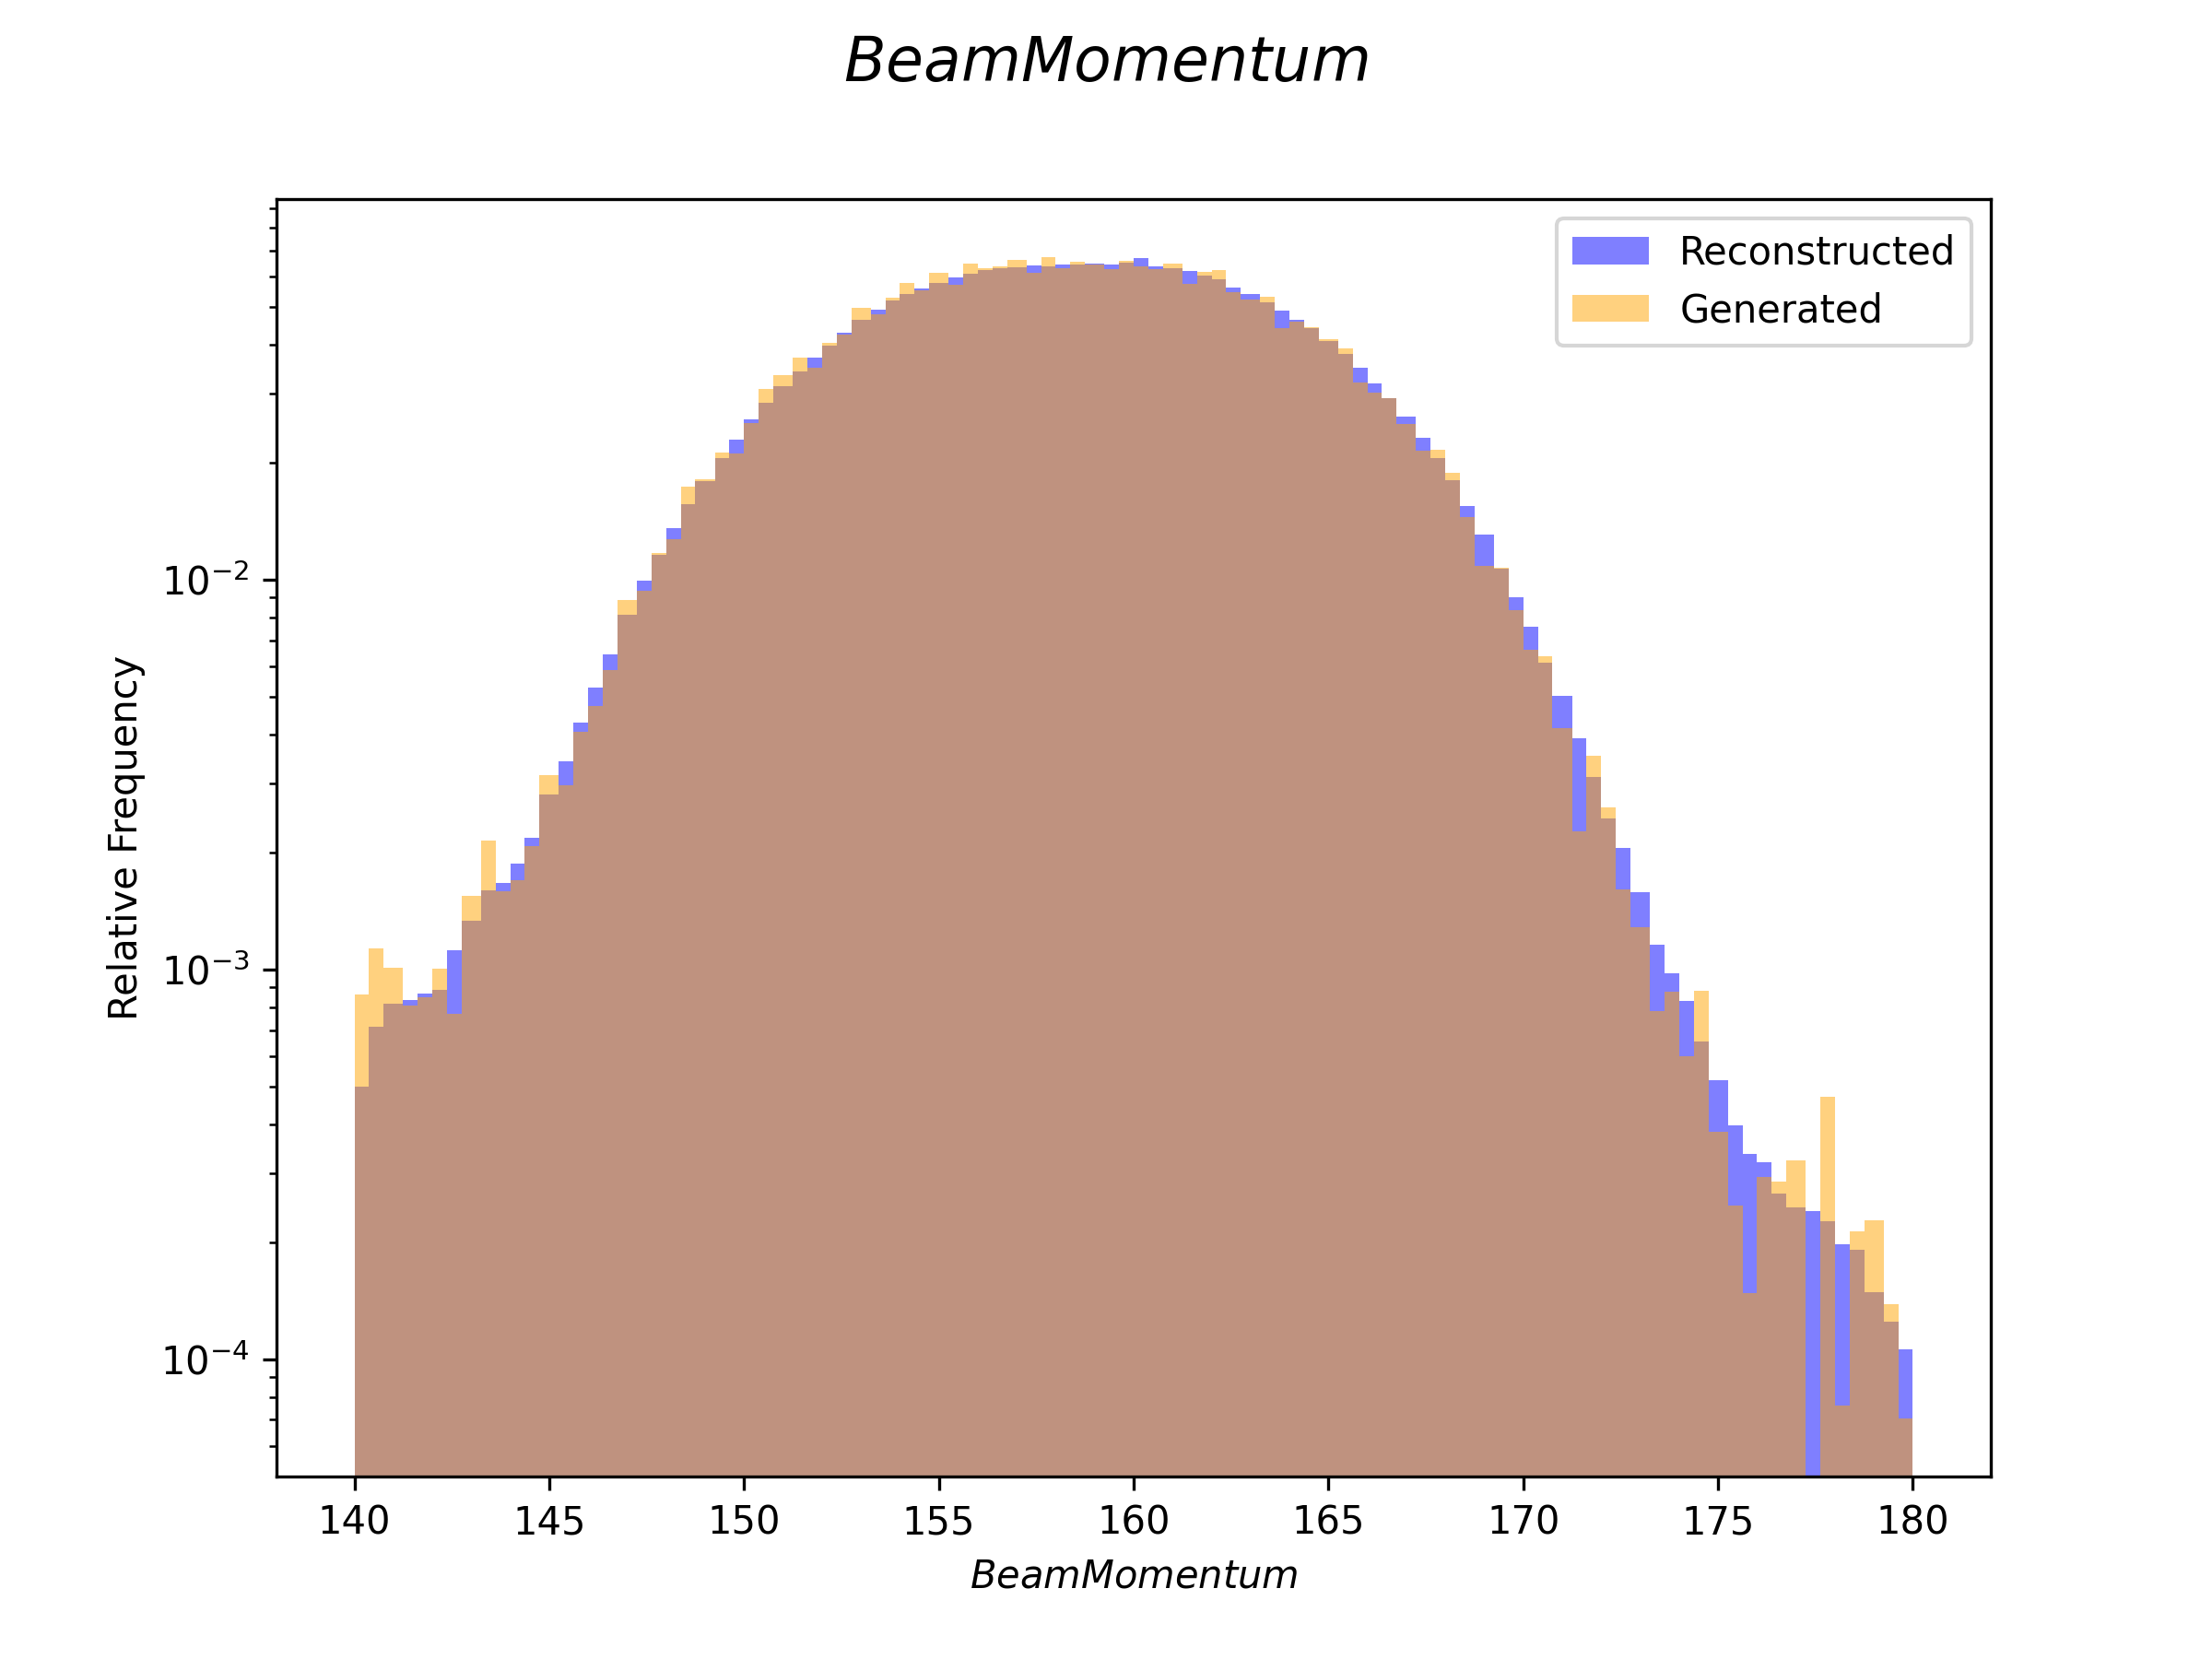
\includegraphics[width=\textwidth]{graphs/hadr_Beam_Momentum.png}
        \caption{Histogram for $Mom_{mup}$}
        \label{fig:had_Momentum_mup}
    \end{subfigure}
    \caption{Histograms for $Mom_{mu}$ and $Mom_{mup}$}
\end{figure}

\begin{figure}[H]
    \centering
    \begin{subfigure}[b]{0.45\textwidth}
        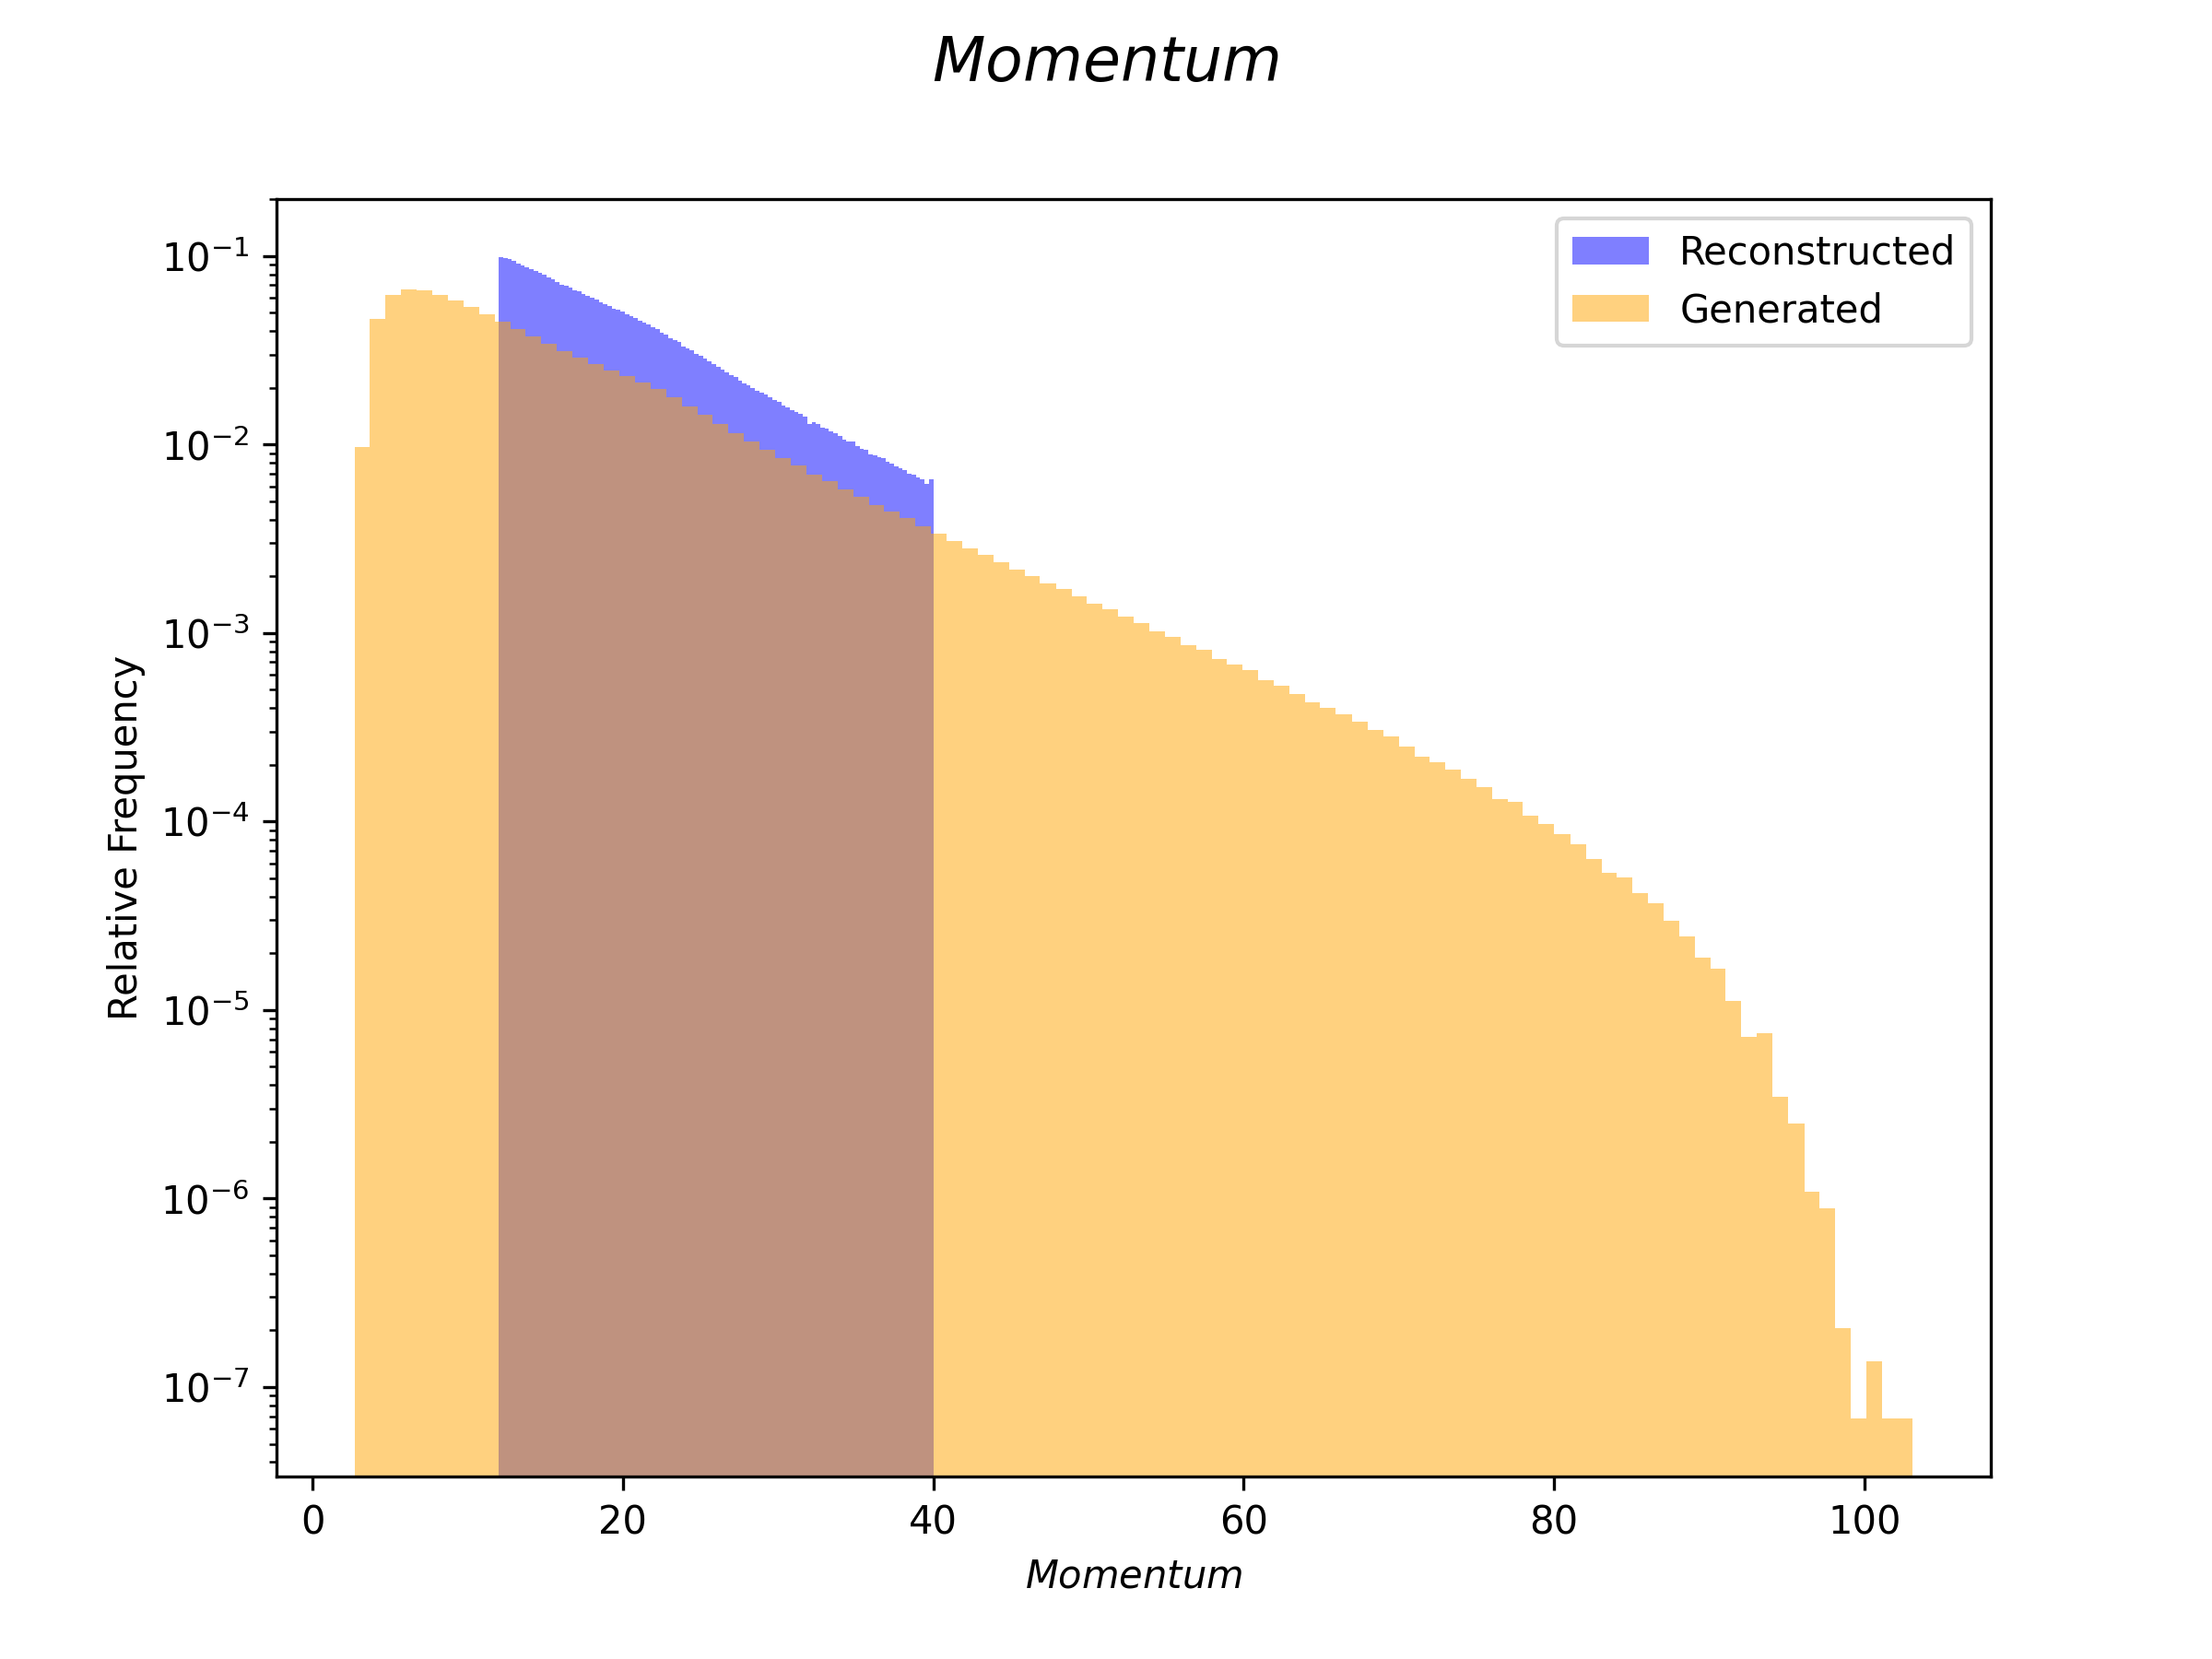
\includegraphics[width=\textwidth]{graphs/hadr_Momentum.png}
        \caption{Histogram for $d_xd_zmup$}
        \label{fig:had_Angle_mu_2}
    \end{subfigure}
    \hfill
    \begin{subfigure}[b]{0.45\textwidth}
        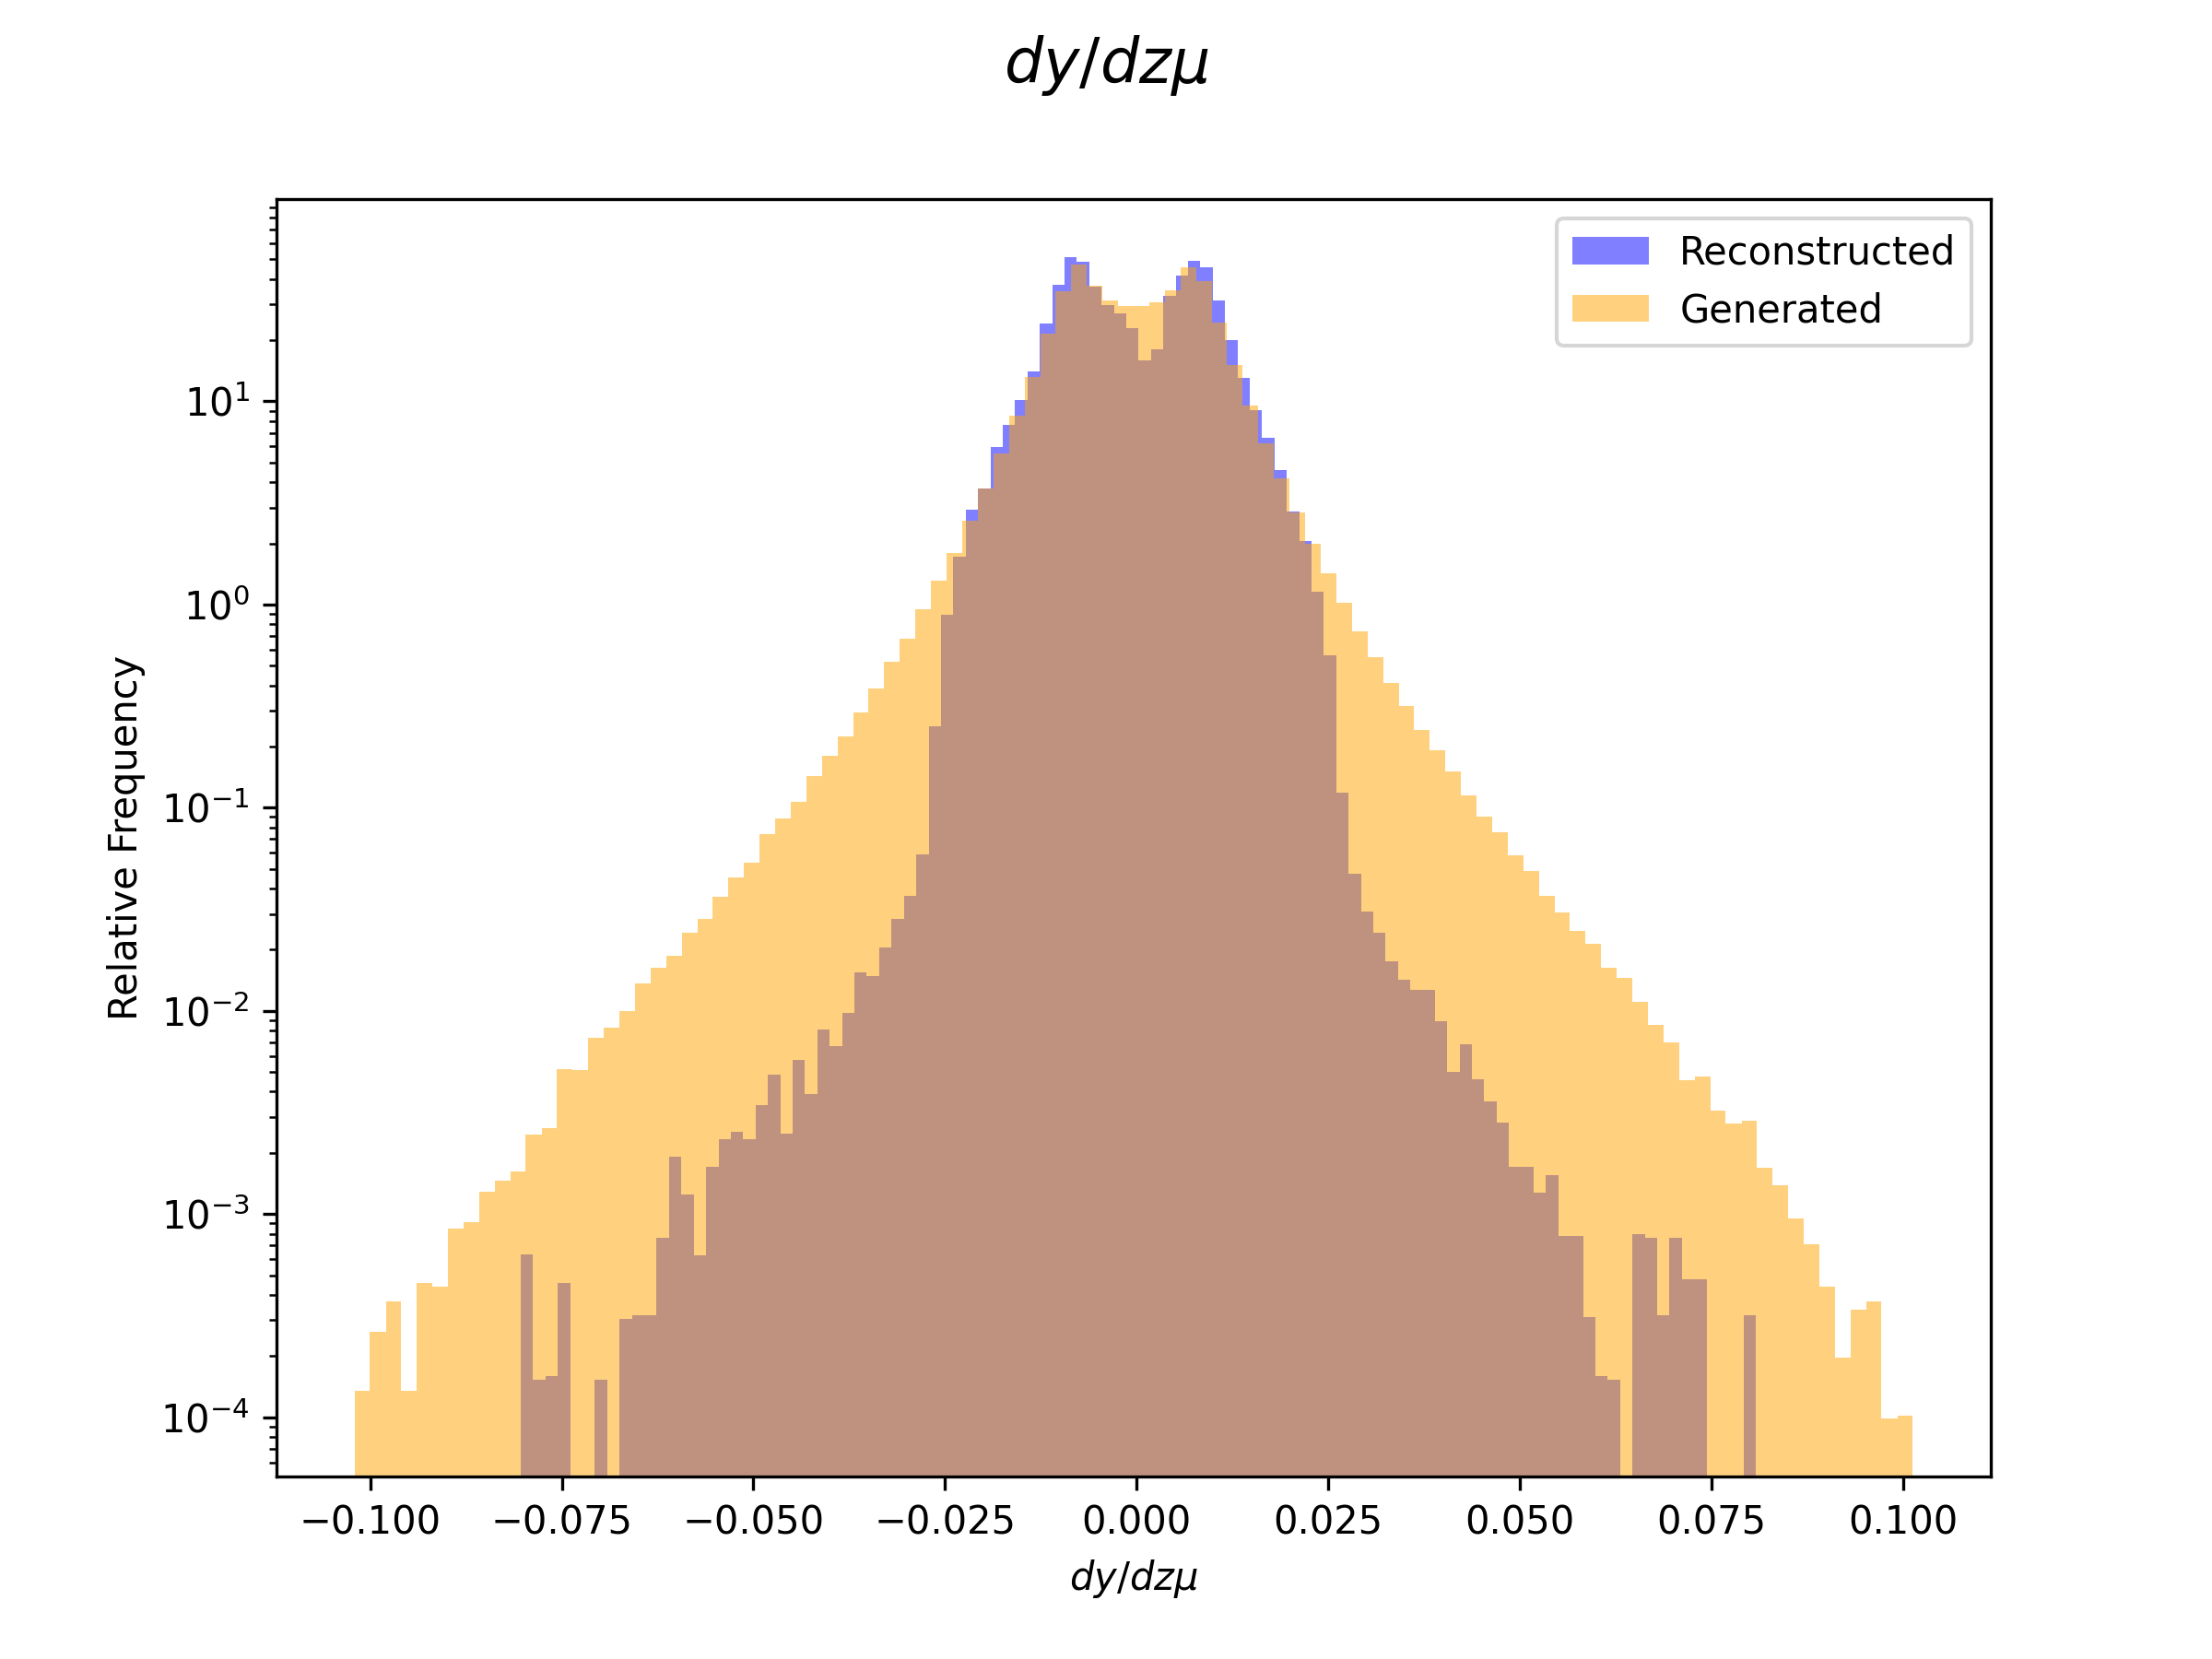
\includegraphics[width=\textwidth]{graphs/hadr_dy_dz_mu.png}
        \caption{Histogram for $d_yd_z \mu p$}
        \label{fig:had_Angle_u_3}
    \end{subfigure}
    \caption{Histograms for $d_xd_zmup$ and $d_yd_z \mu p$}
\end{figure}

\begin{figure}[H]
    \centering
    \begin{subfigure}[b]{0.45\textwidth}
        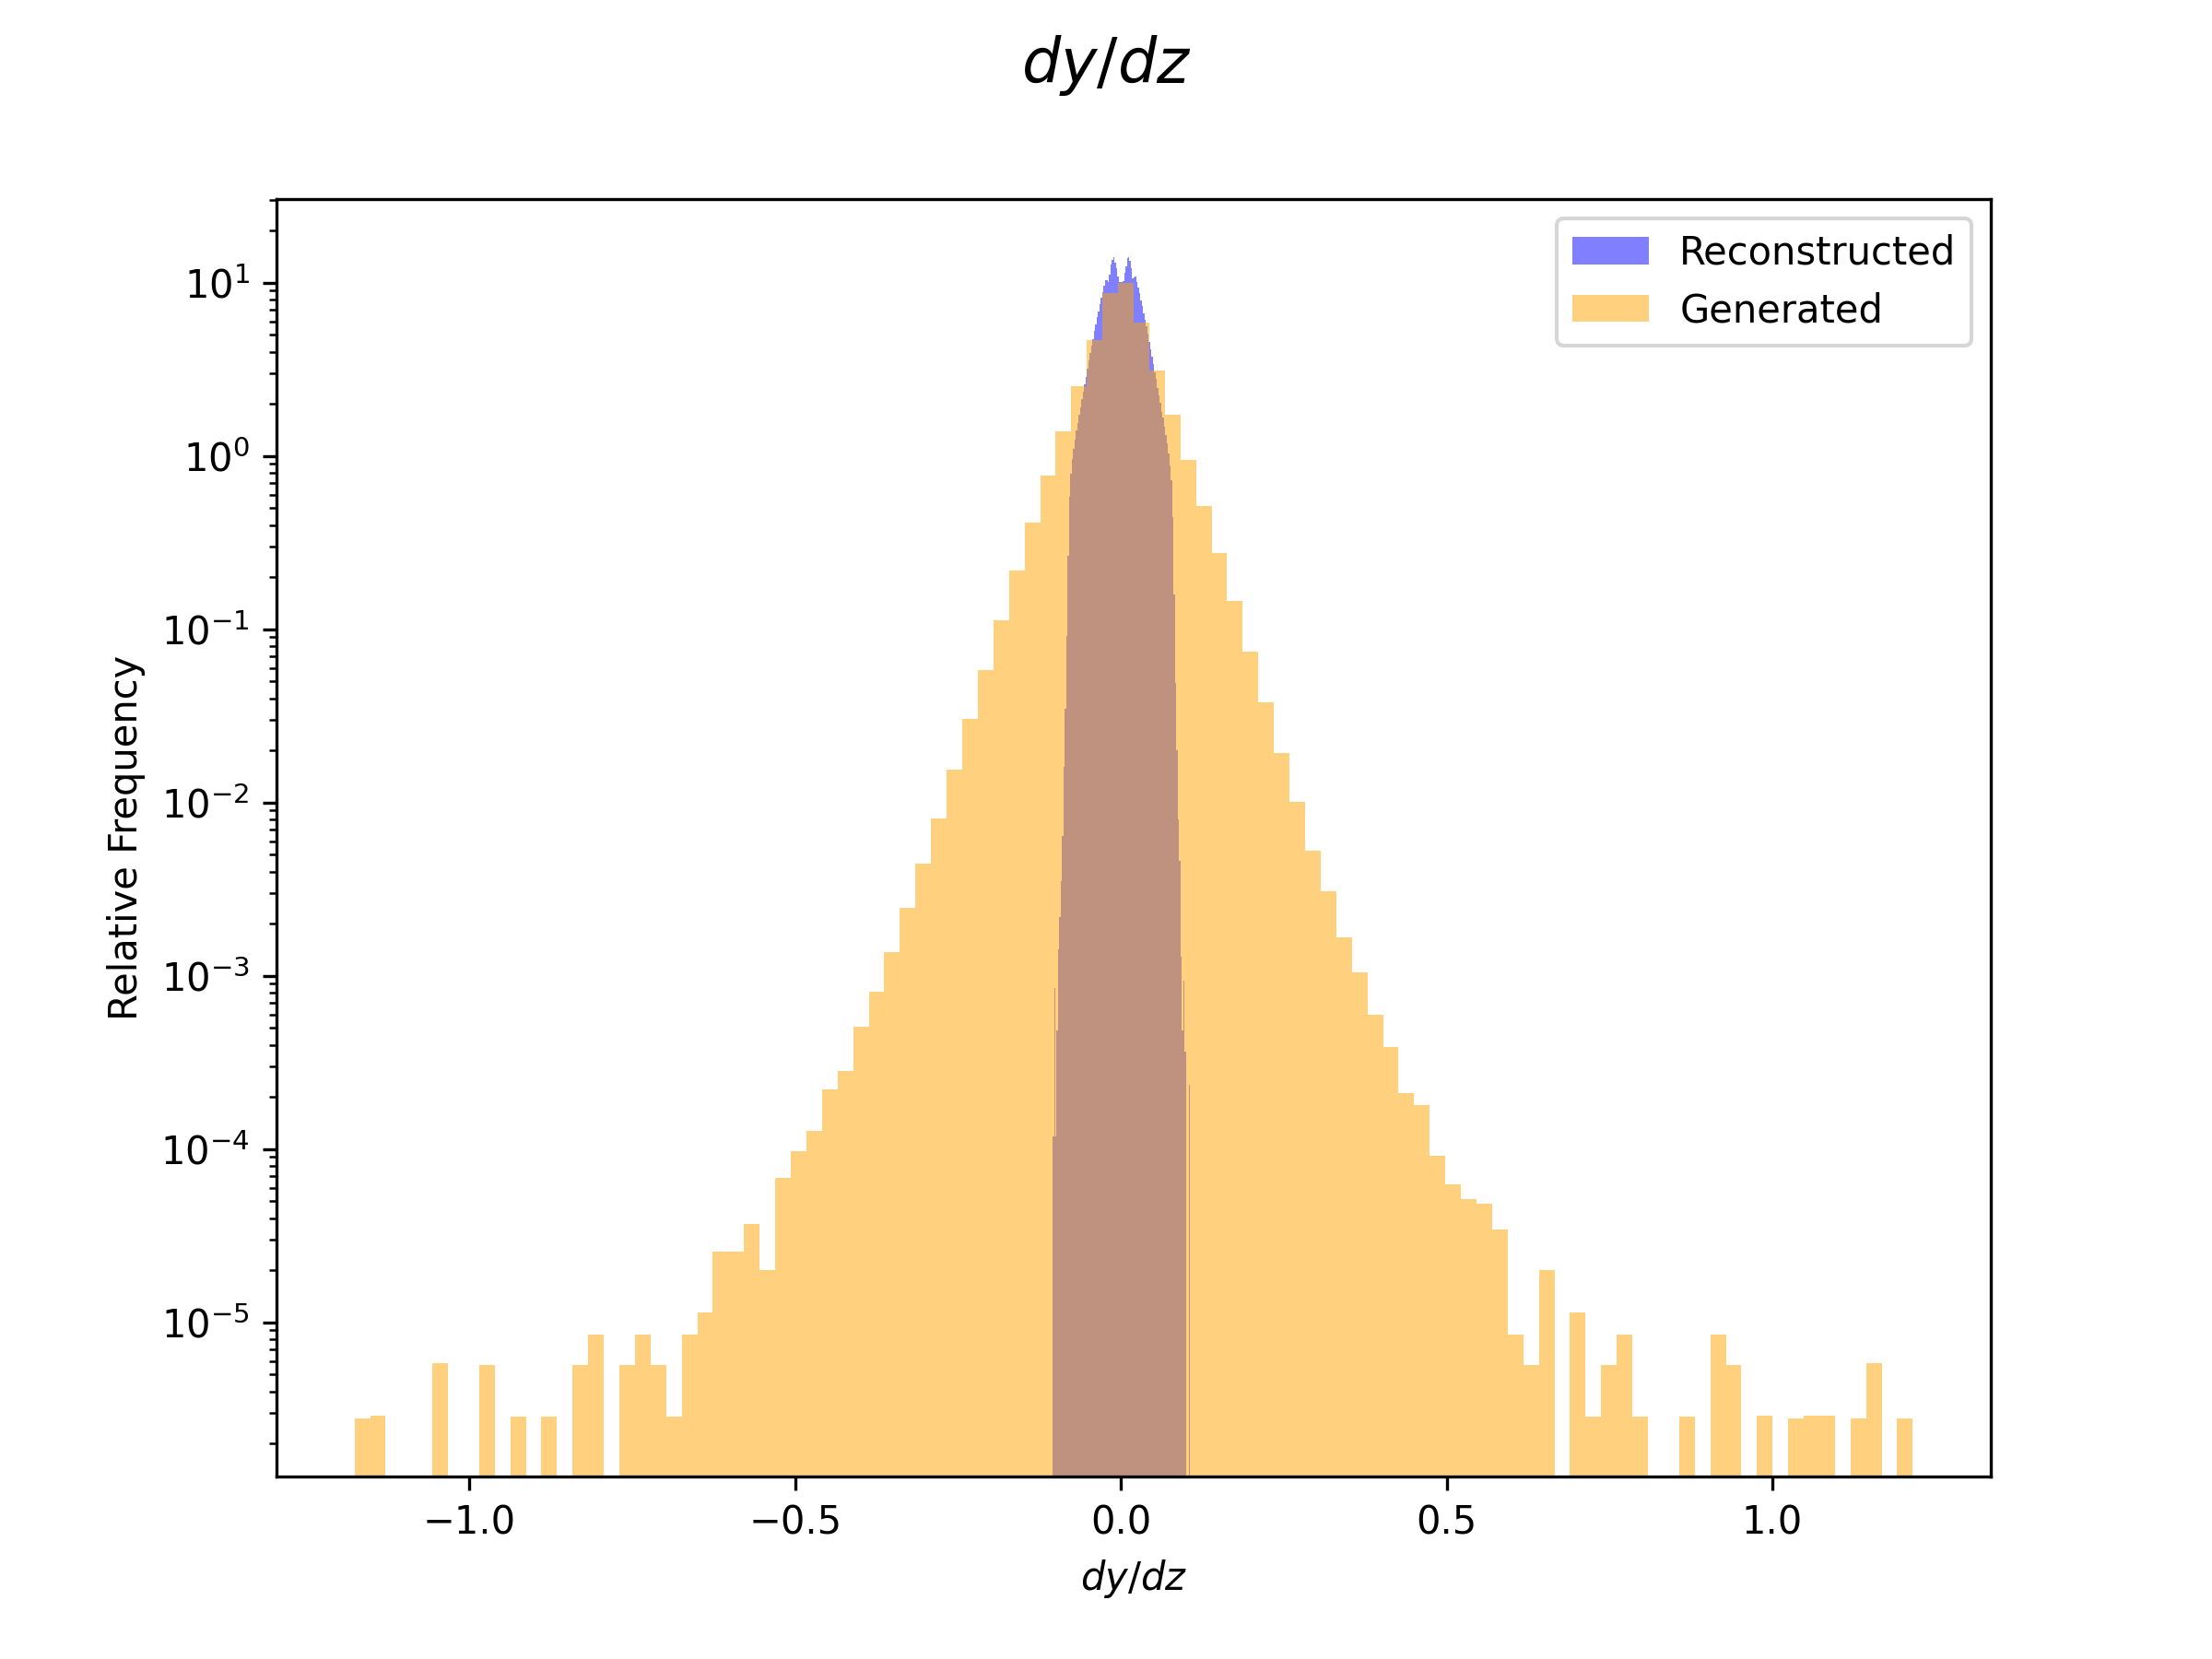
\includegraphics[width=\textwidth]{graphs/hadr_dy_dz.png}
        \caption{Histogram for $d_yd_z$}
        \label{fig:had_Angle_m}
    \end{subfigure}
    \hfill
    \begin{subfigure}[b]{0.45\textwidth}
        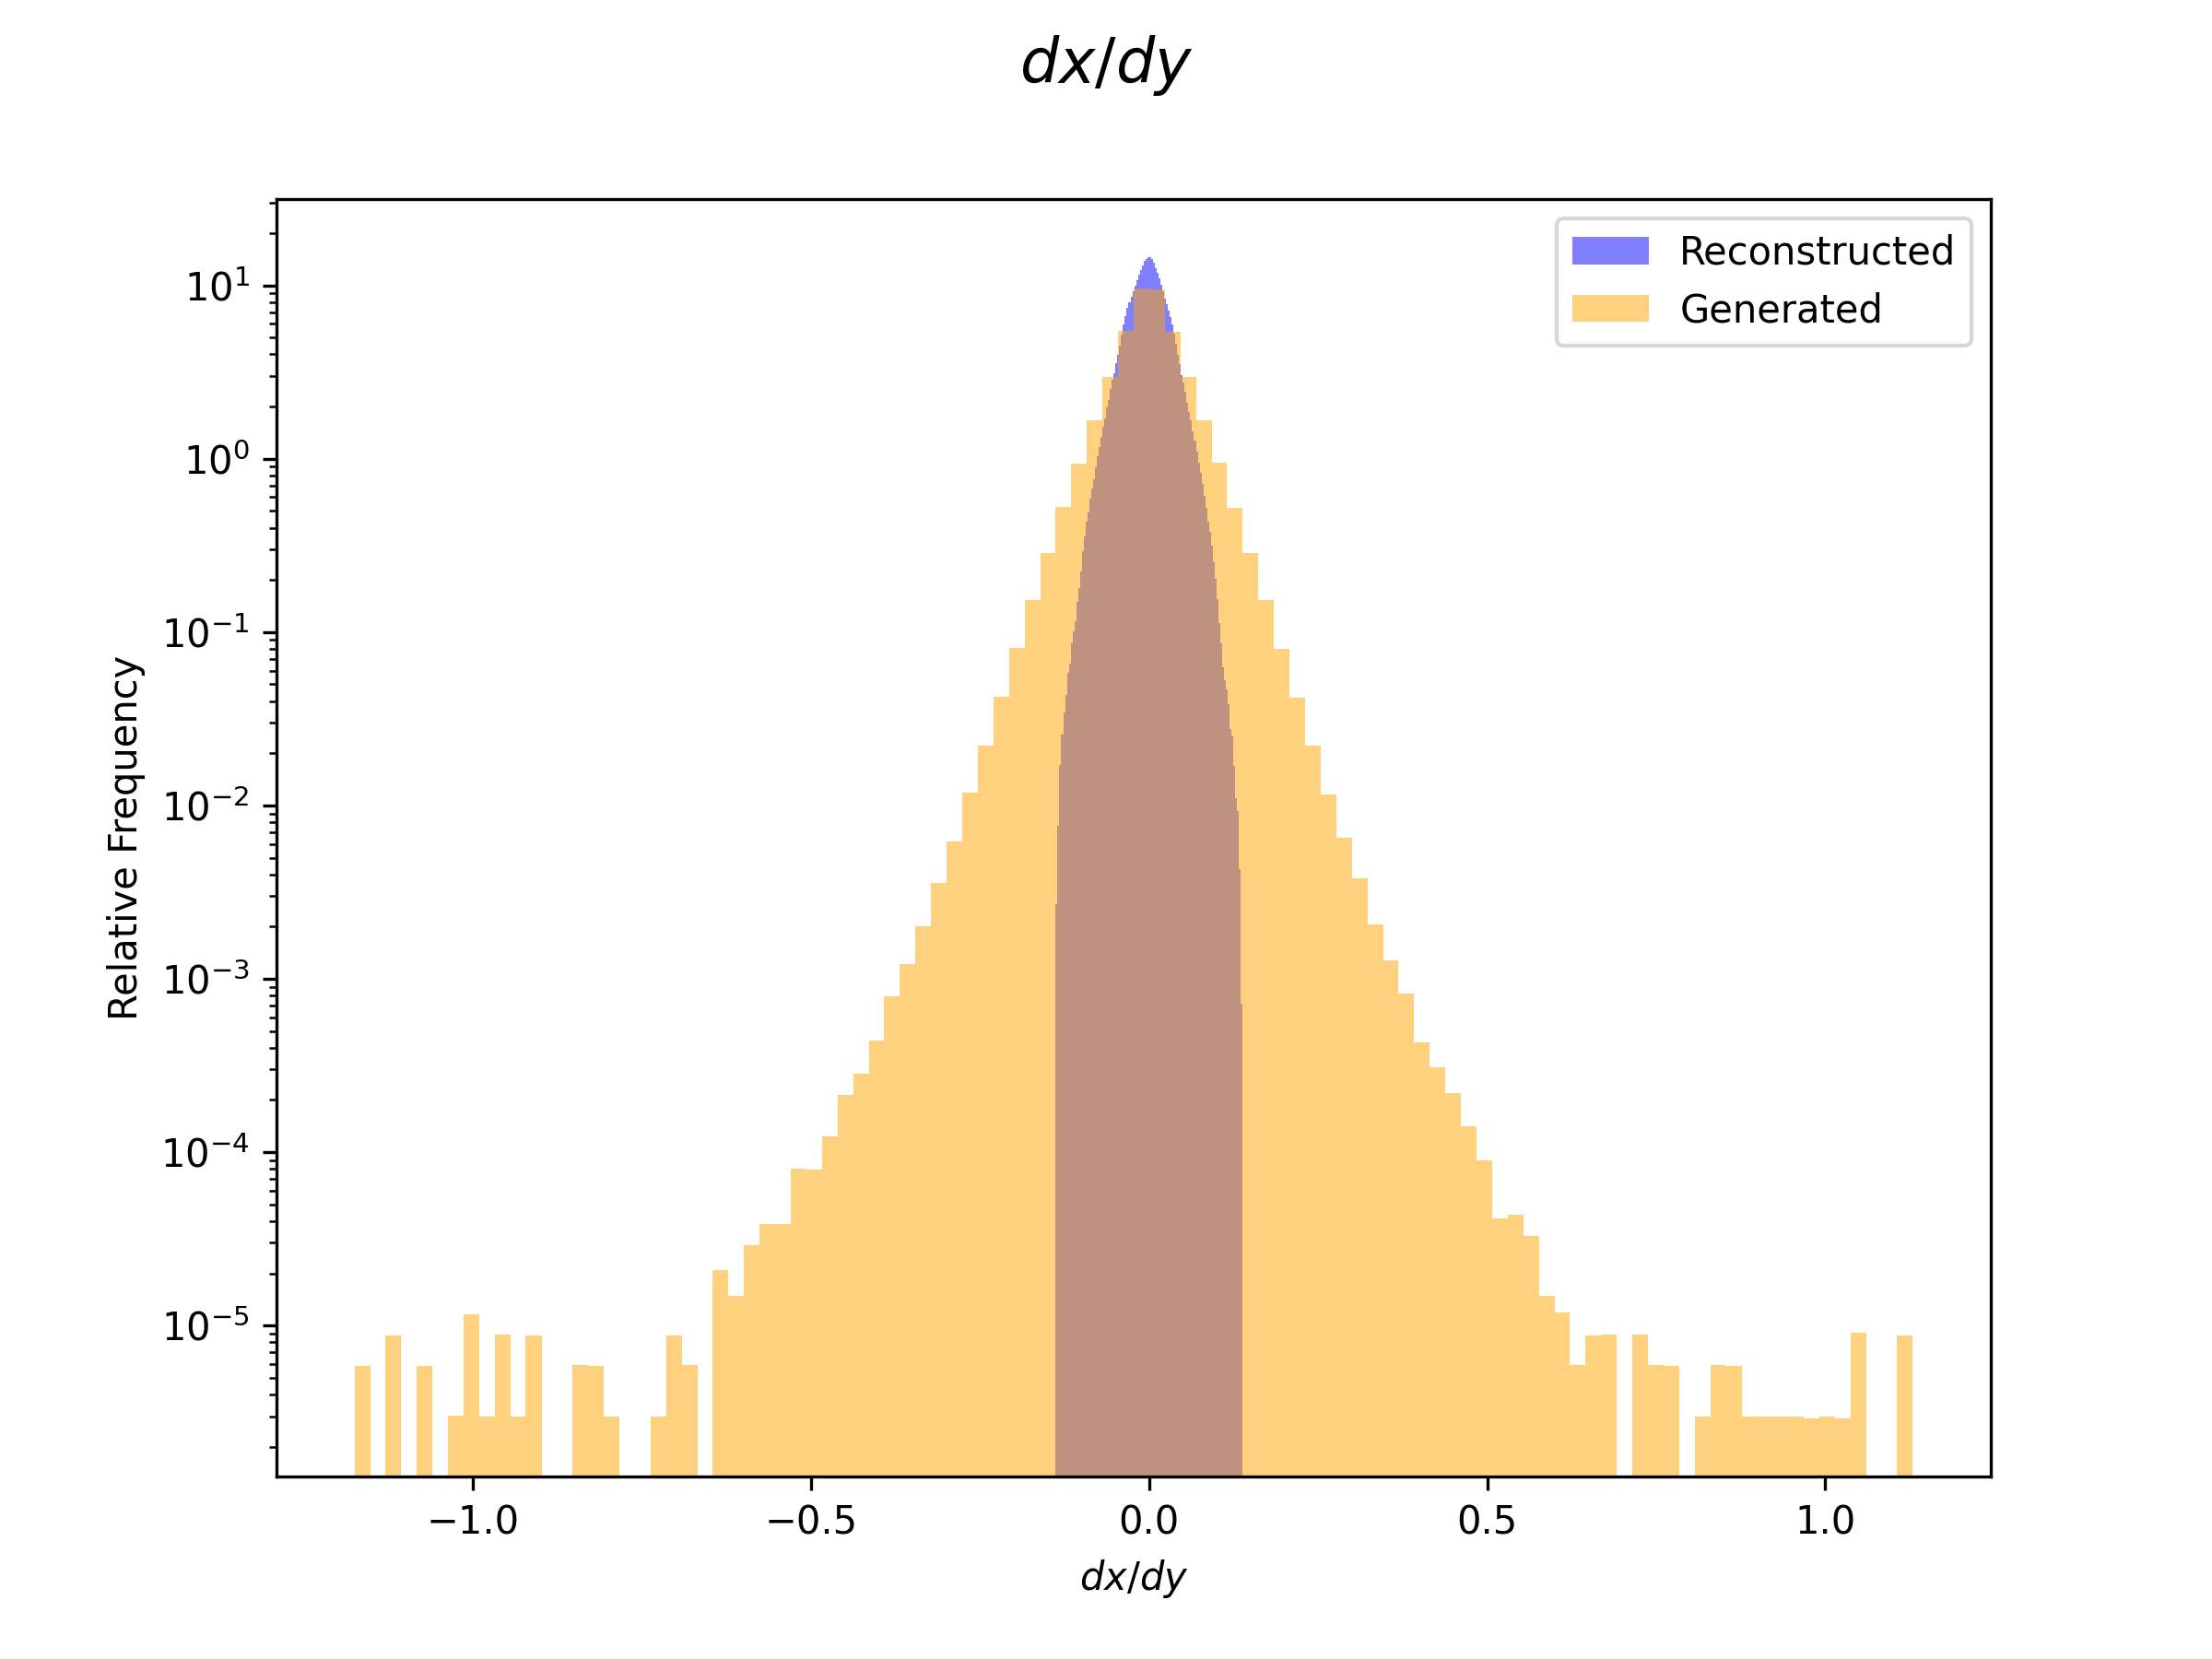
\includegraphics[width=\textwidth]{graphs/hadr_dx_dy.png}
        \caption{Histogram for $d_xd_z$}
        \label{fig:had_Angle}
    \end{subfigure}
    \caption{Histograms for $d_yd_z$ and $d_xd_z$}
\end{figure}

\begin{figure}[H]
    \centering
    \begin{subfigure}[b]{0.45\textwidth}
        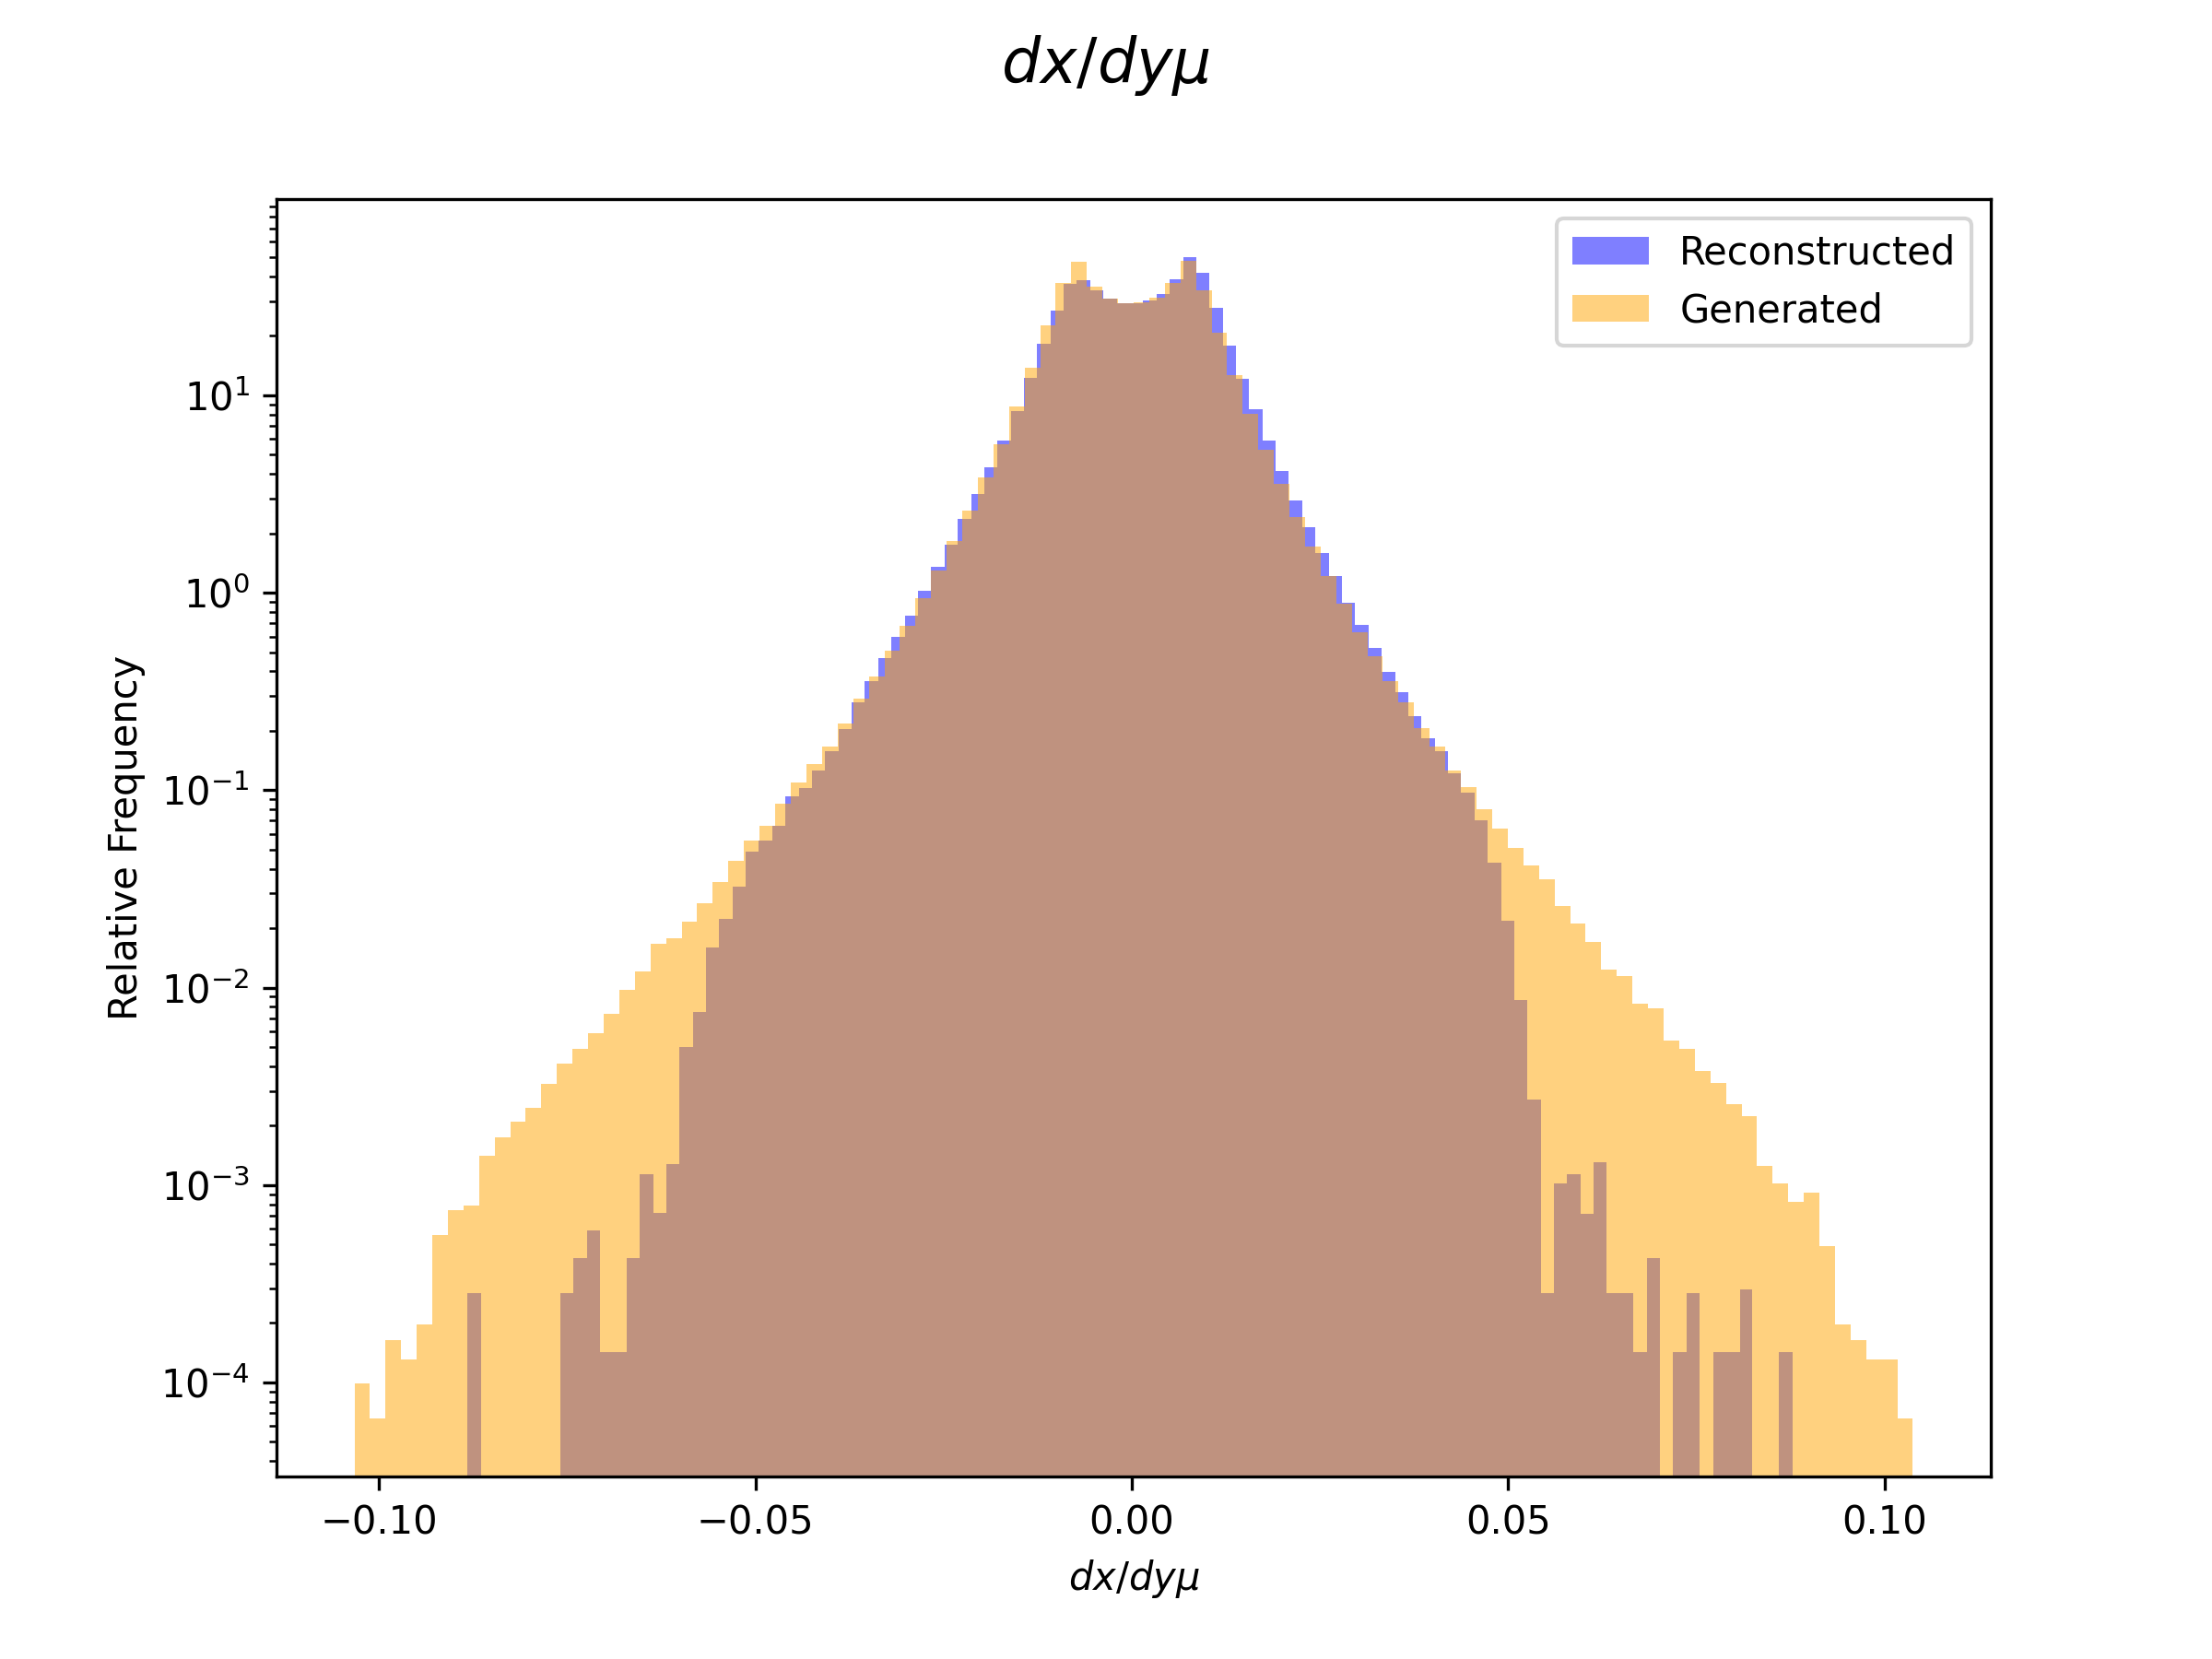
\includegraphics[width=\textwidth]{graphs/hadr_dx_dy_mu.png}
        \caption{Histogram for $d_xd_z \mu$}
        \label{fig:had_Angle_mu}
    \end{subfigure}
    \hfill
    \begin{subfigure}[b]{0.45\textwidth}
        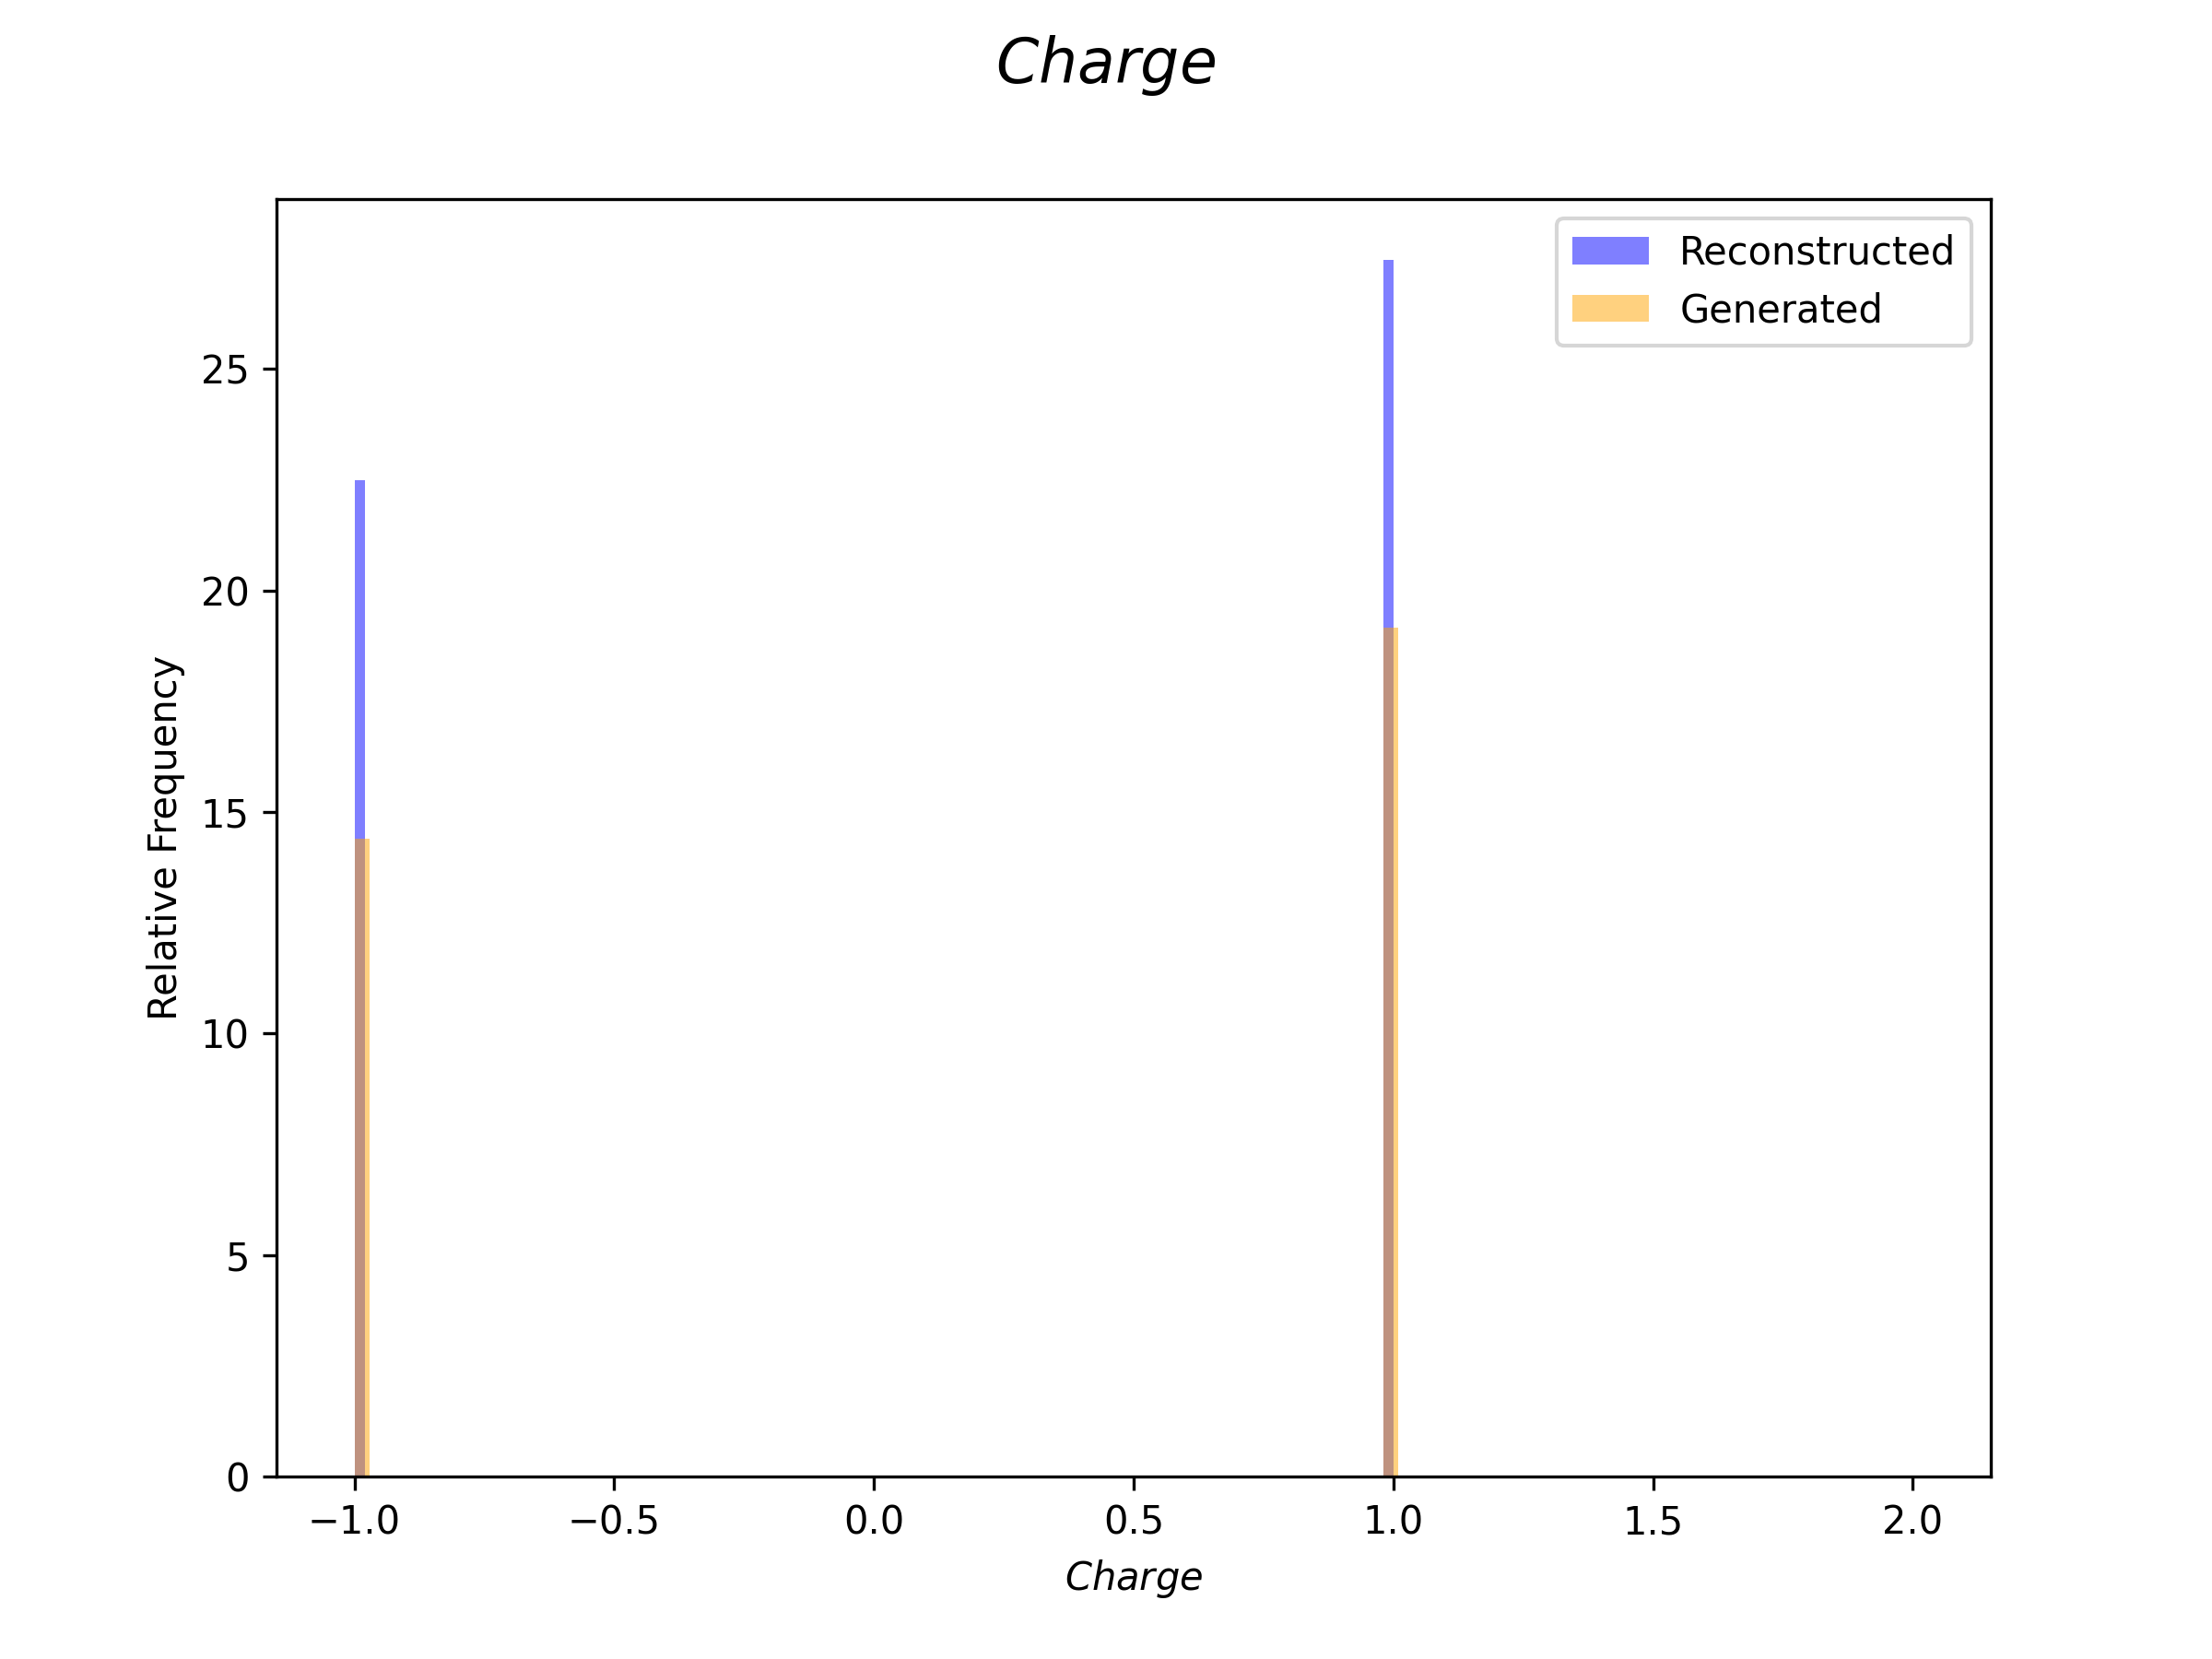
\includegraphics[width=\textwidth]{graphs/hadr_Charge.png}
        \caption{Histogram for Charge}
        \label{fig:had_mom}
    \end{subfigure}
    \caption{Histograms for $d_xd_z \mu$ and Charge}
\end{figure}

For the Hadrons events, we are going to use a 3D tensor for the $X$, $Y$ and $Z$ variables to further evaluate the performance of the models (explained in section METER AQUI).
Since we cannot plot a histogram that allows us to visualize this '3D histogram', no image will be presented here, but the it will be used in the chi-squared test.
One could plot several 2D histograms, one for each $Z$ value, but that would be very time consuming and not very practical.


\subsection{Correlation between Variables}
In order to check if there is any correlation between the variables, we plotted the correlation matrix with the Pearson Coefficient for the Inclusive and Hadrons events.
This is important because if there is a high correlation between two variables, it means that they are redundant, and therefore, one of them can be removed, 
which simplifies the training of the Neural Network, reduces the number of parameters (reducing the training time) and avoids overfitting.
The results are shown in the figures below:

\begin{figure}[H]
    \centering
    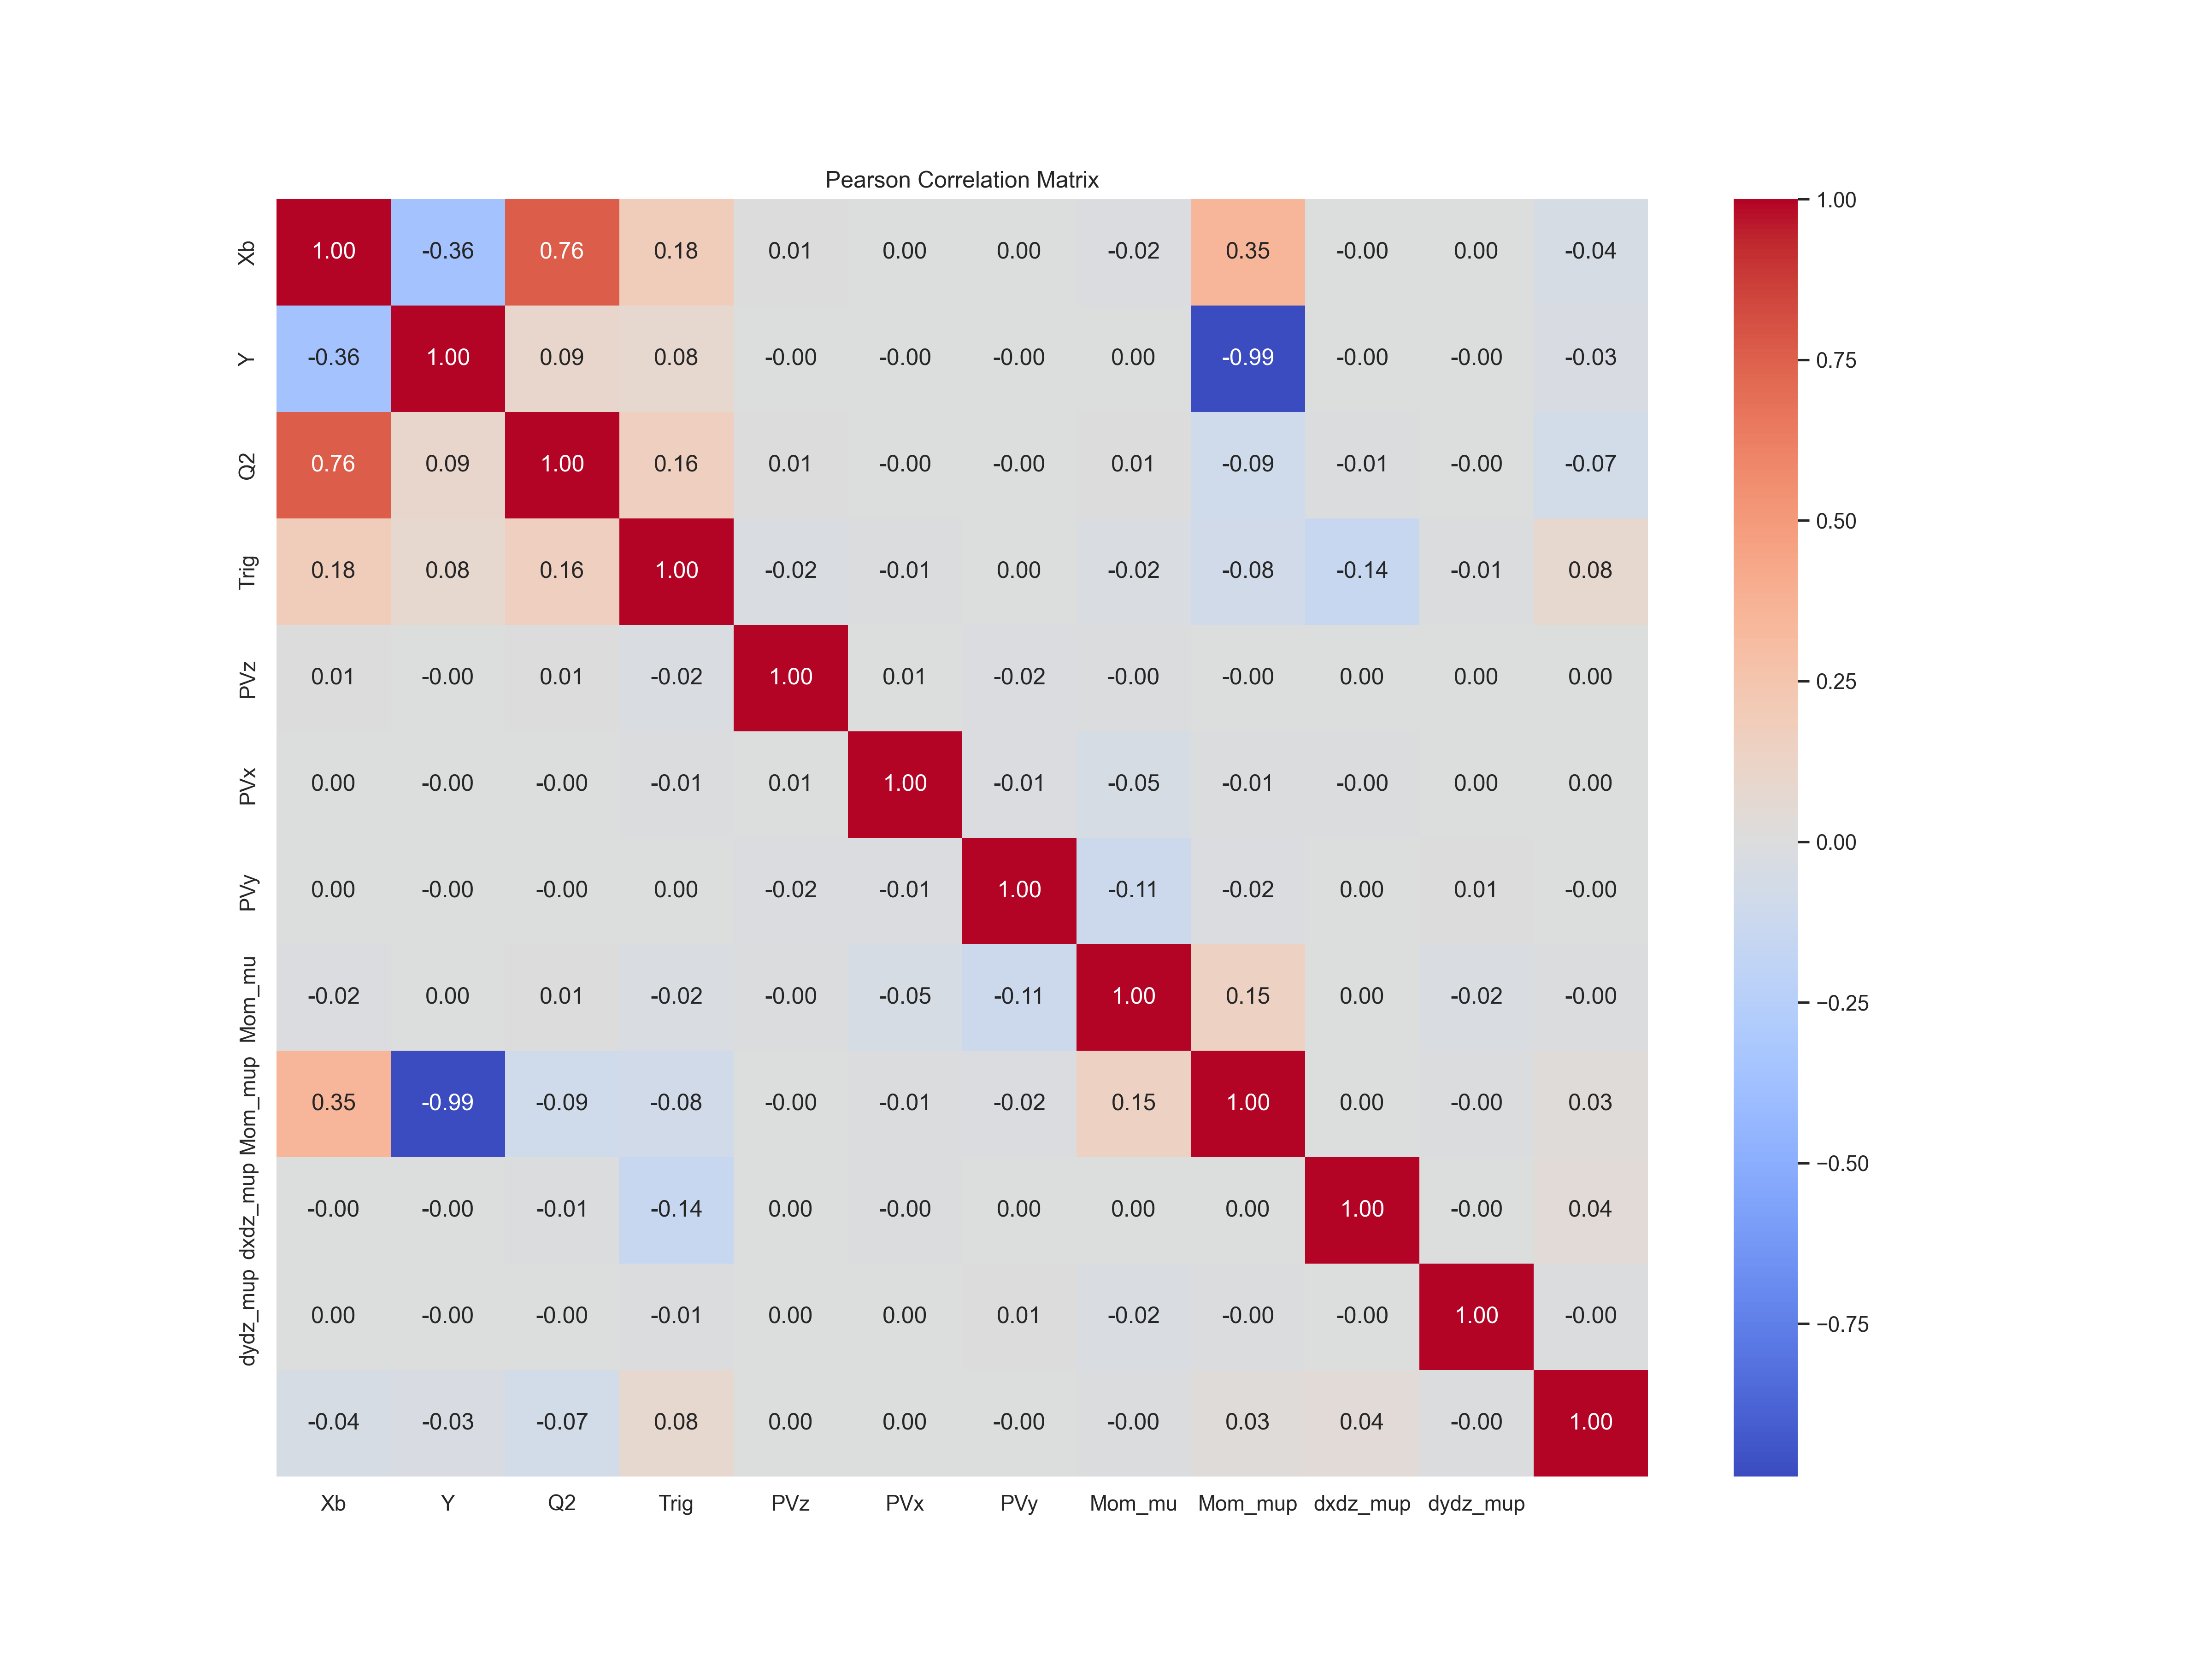
\includegraphics[width=0.9\textwidth]{graphs/inclusive_correlation_matrix.png}
    \caption{Correlation Matrix for the Inclusive Events}
    \label{fig:inclusive_correlation_matrix}
\end{figure}

\begin{figure}[H]
    \centering
    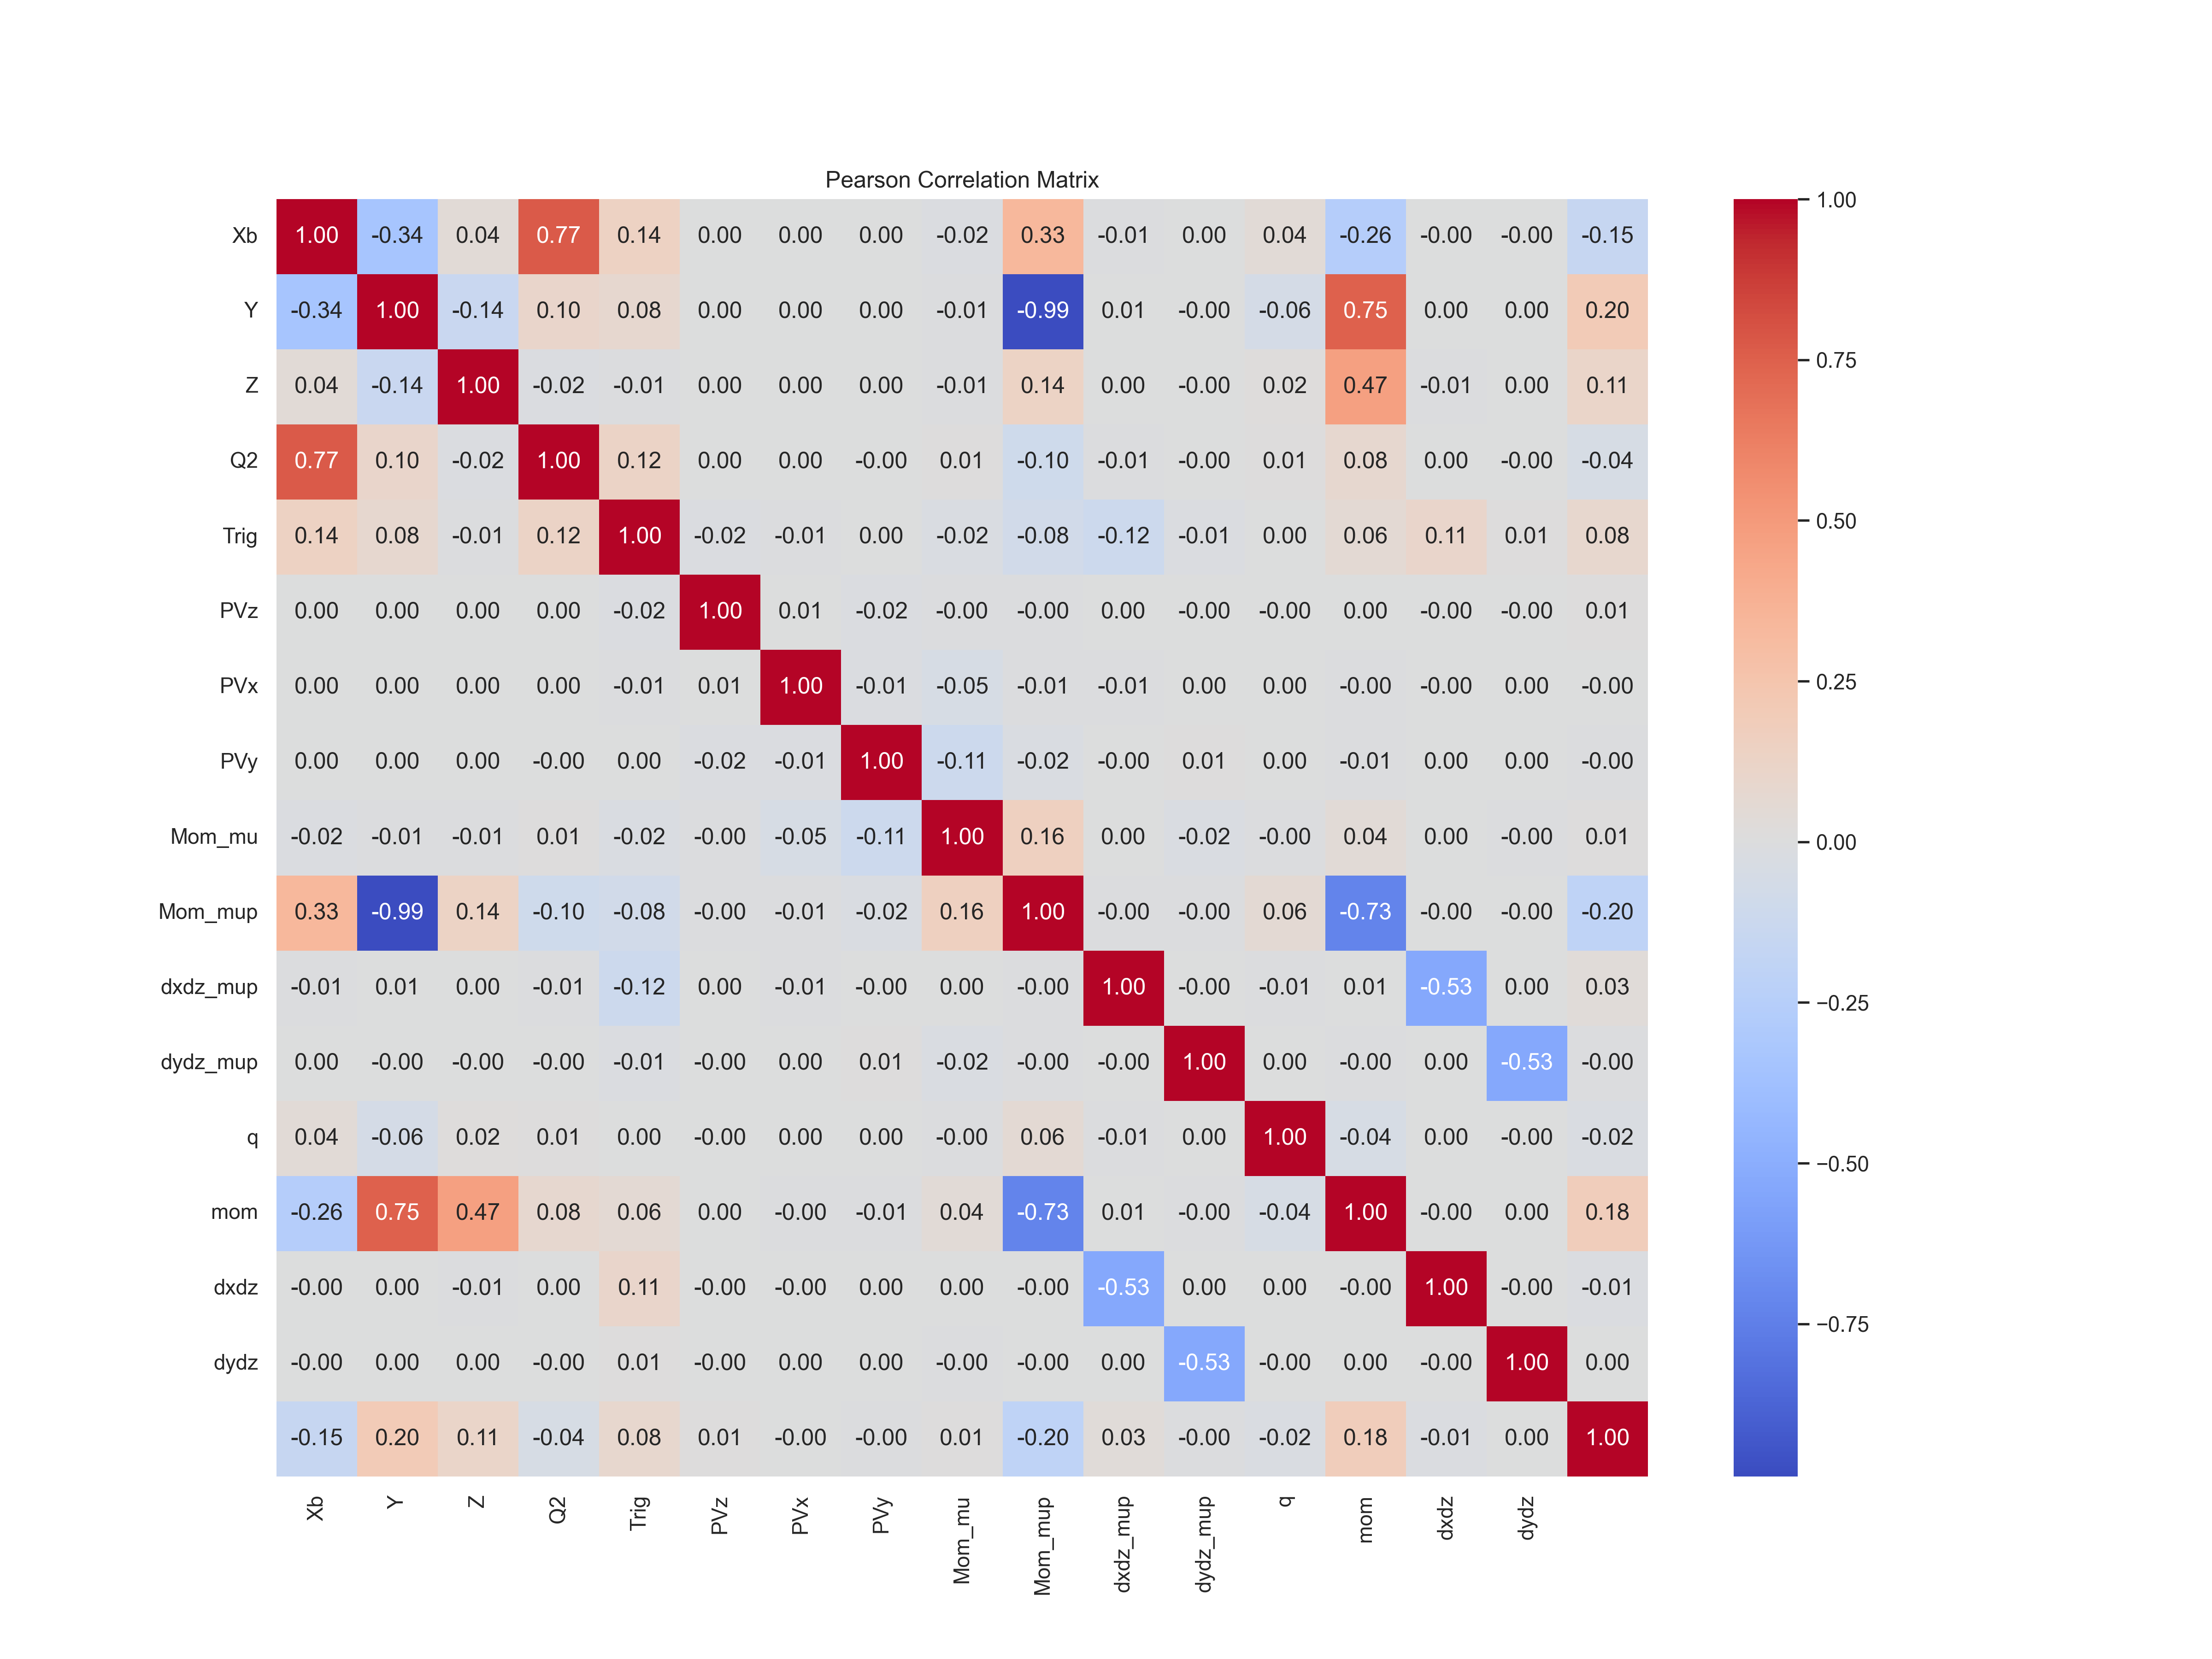
\includegraphics[width=0.9\textwidth]{graphs/hadron_correlation_matrix.png}
    \caption{Correlation Matrix for the Hadron Events}
    \label{fig:hadron_correlation_matrix}
\end{figure}


As seen in the figures above, there is a high correlation between $Y$ and $Mom_{mup}$, with
a pearson correlation coefficient of -0.99 for both types of events. Therefore, one of them can be removed from the training
of the Neural Network. Since $Mom_{mup}$ and $Y$ have the same correlation coefficient, we decided to remove $Mom_{mup}$ from the training of the Neural Network,
since from the physics point of view, $Y$ is more important than $Mom_{mup}$, since it is the variable that gives us the virtual photon energy fraction of the initial momentum. 

\subsection{Weighting}
As previously mentioned, the datasets from the Monte Carlo and the reconstructed data exhibit variations in the number of events. The Monte Carlo dataset contains a larger number of events compared to the reconstructed data. Consequently, we needed to address this disparity to ensure fair and effective training and testing of the Neural Network.

Our approach involved a two-step process. Initially, we trained the Neural Network using only a small percentage of the data to fine-tune the hyperparameters. Subsequently, we performed the main training using the entire dataset and tested the model with the full dataset. However, due to the differing event counts in each dataset, it was imperative to balance the data during both stages of training and testing.

While fine-tuning the hyperparameters, it was not feasible to utilize an equal count of events from the Reconstruction and Generation datasets, given their inherent numerical differences. Therefore, our solution involved using a proportional representation by employing percentages of the data. This approach is crucial because using an event count-based method would result in varying proportions of accepted and rejected events in the training and testing datasets, which could skew the model's performance evaluation.


\section{Neural Network Architecture and Training}

\subsection{Models Architecture, Hyperparameters and Metrics}

\subsubsection{Architecture of the Models}

For the Neural Networks models we used the PyTorch framework, which is an open source machine learning library based on the Torch library, used for applications such as computer vision and natural language processing.
For the models architecture, two different models were used, one with 3 hidden layers, two GELU activation functions and two dropout layers, and another with 6 hidden layers, 5 GELU activation functions and 3 dropout layers.
The choice of the number of hidden layers and the number of neurons in each layer was done by trial and error, and the same applies to the choice of the dropout rate. 
The GELU activation function was chosen because it is the one that gave the best results, and the same applies to the choice of the optimizer, which was the Adam optimizer.
These two models were chosen because they are the ones that gave the best results and also because there was the need to see the difference between a not so deep model and a deeper model.
The hyperparameters used for the training of the models were the following:
\begin{itemize}
    \item Learning Rate: 0.01
    \item Epochs: 10
    \item Batch Size: 1
\end{itemize}

For the loss function, we used the Binary Cross Entropy Loss, which is the most common loss function used for binary classification problems.
Despite the fact that this set of data might be familiar with a binary classification problem, since we are trying to predict if an event will be accepted or rejected,
we are not doing a binary classification problem, since we are not trying to classify the events, but rather predict the acceptance of the COMPASS/AMBER.
Therefore, there was no need to round the output of the Neural Network to 0 or 1, since the output of the Neural Network is a number between 0 and 1, which represents the probability of the event being accepted.

\subsection{Evaluation of the Models}

During the training of the models, we printed the accuracy and the loss as metrics to evaluate part of the performance of the models.
But since the accuracy and loss are not the best metrics to evaluate the performance of the models in this type of problem, the chi-squared test was used to evaluate the performance of the models.
The chi-squared test is a statistical hypothesis test that is used to evaluate how well a set of data fits a model. In this case, the model is the Neural Network, and the data is the data used for the training and testing of the Neural Network.
For this particular case, the chi-squared was applied to:
\begin{itemize}
    \item Hadrons: 3D histogram with $X$, $Y$ and $Z$ variables
    \item Inclusive: 2D histogram with $X$ and $Y$ variables
\end{itemize}

The chi-squared used was defined as:

\begin{equation}
    \chi^2 = \sum_{i=1}^{N} \frac{(\frac{r - A_{nn}}{g - A_{nn}})^2}{err}
\end{equation}
    
where $r$ is the number of reconstructed events in the bin, $g$ is the number of generated events in the bin, $A_{nn}$ is the output of the Neural Network for the bin and $err$ is the error of the bin, which is defined as:

\begin{equation}
    err = \frac{1}{g^2}\sqrt{(\frac{2r^2 + g^2}{g^2})^2}
\end{equation}

For Inclusive events, we anticipate a chi-squared value of approximately 45. It's worth noting that the expected value should theoretically be 60 since there are 60 bins. However, due to certain bins appearing to be empty, we are expecting a somewhat lower value.

In the case of Hadron events, we are looking for a chi-squared value of roughly 400. Similarly, the theoretical expected value would be 780, corresponding to the number of bins. Nonetheless, given the presence of apparently empty bins, we anticipate a reduced value.

\subsection{Training, Testing and Results}

During the model training process, an 80\% portion of the dataset was dedicated to training, while the remaining 20\% was allocated for testing. Notably, both models underwent training and testing with the same dataset to ensure a fair basis for comparison.

Throughout the training phase, metrics like accuracy and loss were monitored to assess the models' performance. However, the primary focus was on tracking the chi-squared values, which played a crucial role in identifying the best models.

It's worth noting that the chi-squared values exhibited some instability during training. To account for this, models with chi-squared values were preserved for post-training model selection. This approach allowed for the selection of the best models after considering the chi-squared performance.

Multiple iterations of training were carried out due to the previously mentioned chi-squared instability. To gain insights into the training process, accuracy and loss metrics for both training and testing were plotted and visualized, as depicted in the figure below:

For the Hadron events: 
\begin{figure}[H]
    \centering
    \begin{subfigure}[b]{0.45\textwidth}
        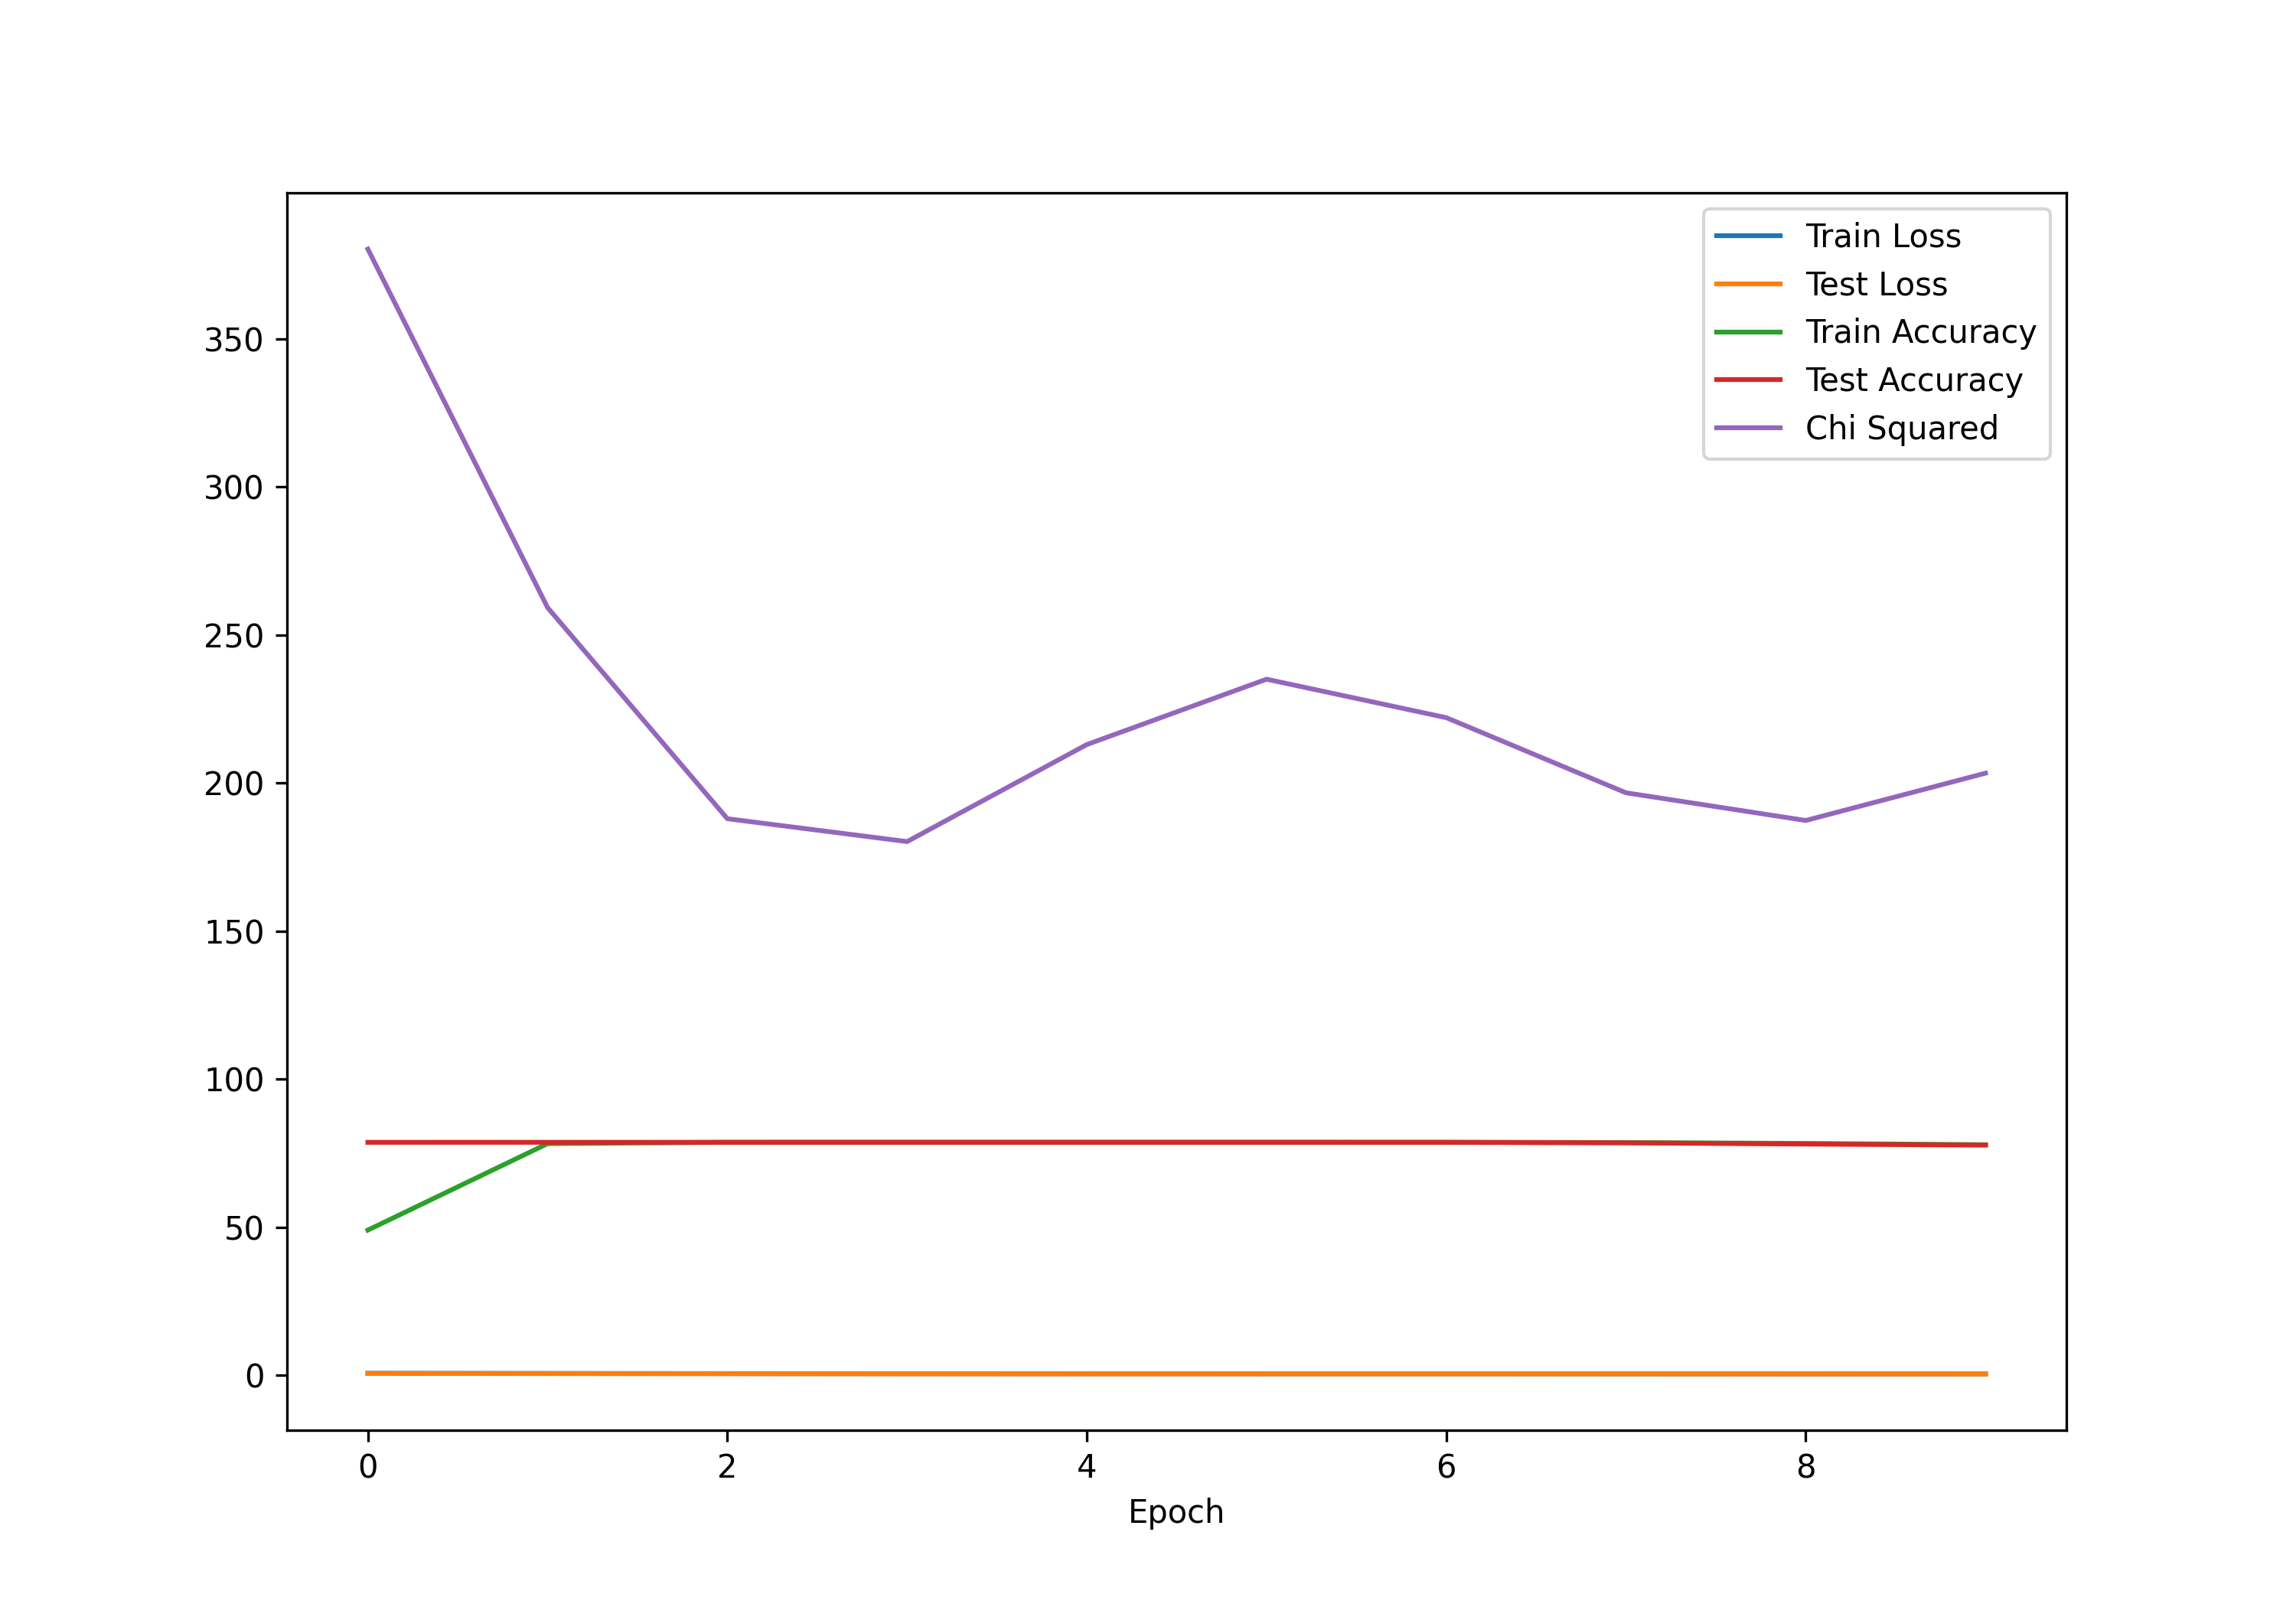
\includegraphics[width=\textwidth]{graphs/nn_hadrons_metrics.png}
        \caption{Shallow Model for Hadron}
        \label{fig:accuracy_loss_hadr}
    \end{subfigure}
    \hfill
    \begin{subfigure}[b]{0.45\textwidth}
        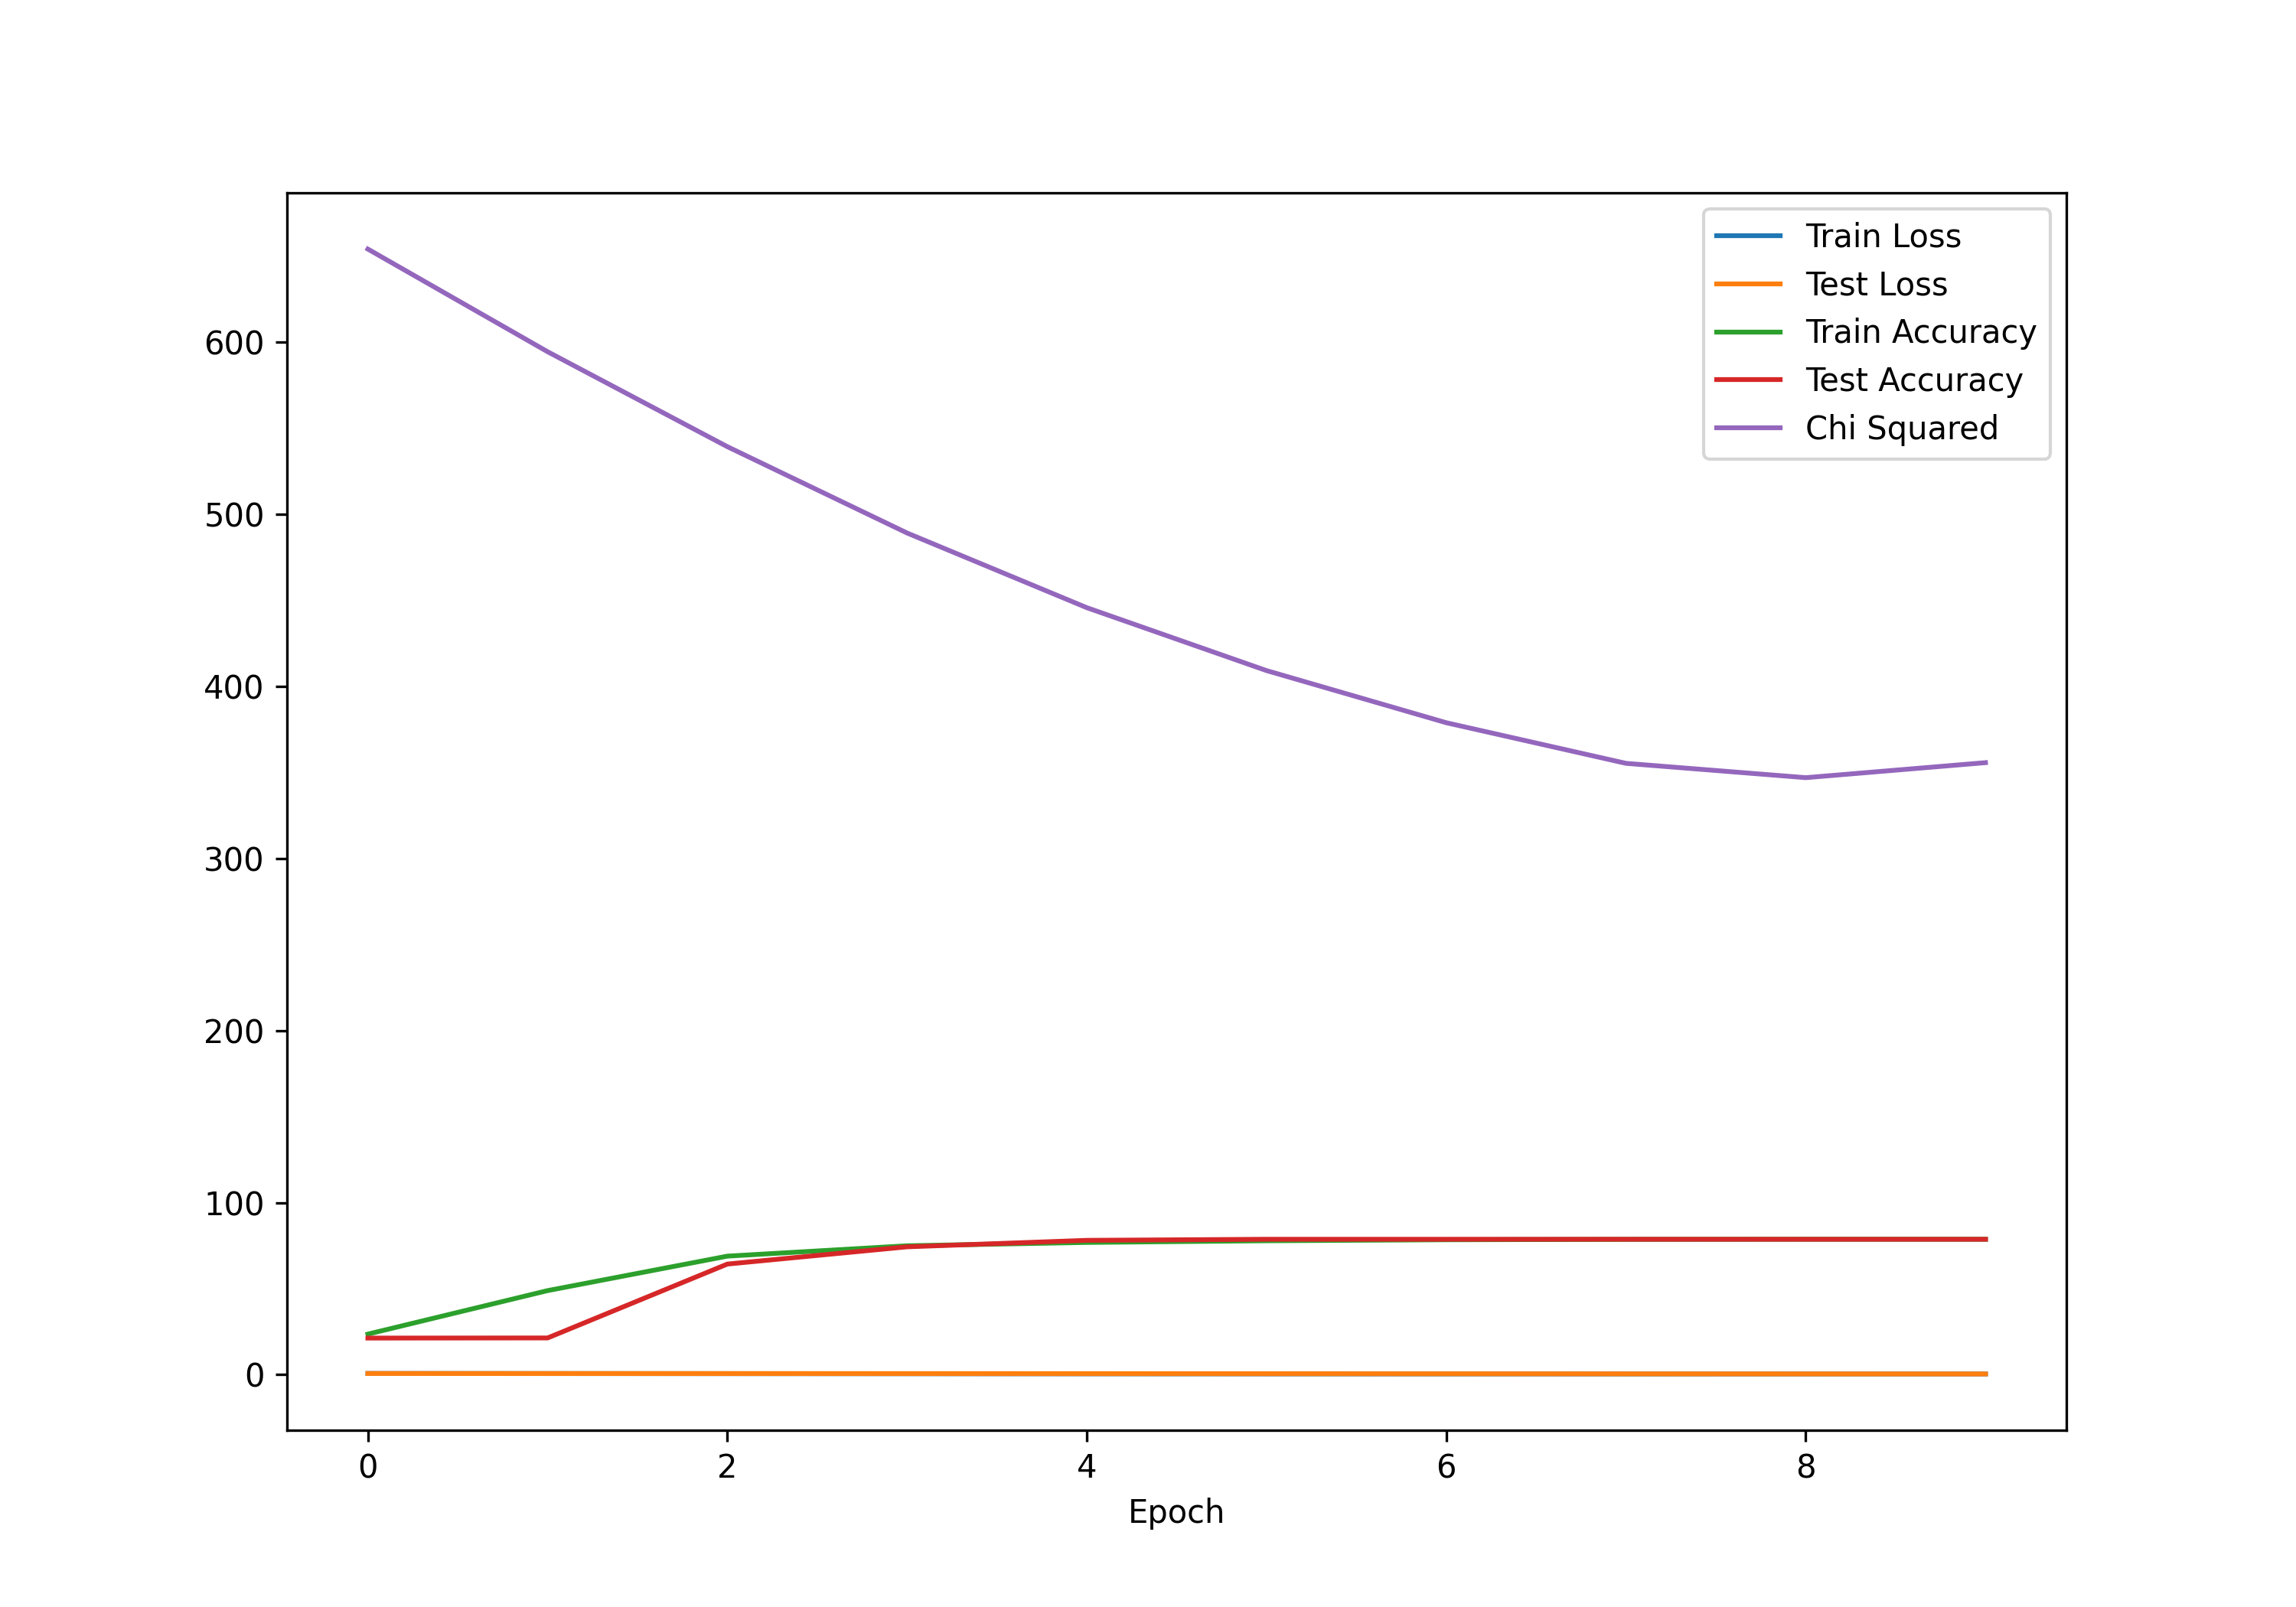
\includegraphics[width=\textwidth]{graphs/nn_hadrons_metrics_deeper.png}
        \caption{Deep Model for Hadron}
        \label{fig:accuracy_loss_hadr_deep}
    \end{subfigure}
    \caption{Comparison of Shallow and Deep Models for Hadron}
\end{figure}

For the Inclusive events:
\begin{figure}[H]
    \centering
    \begin{subfigure}[b]{0.45\textwidth}
        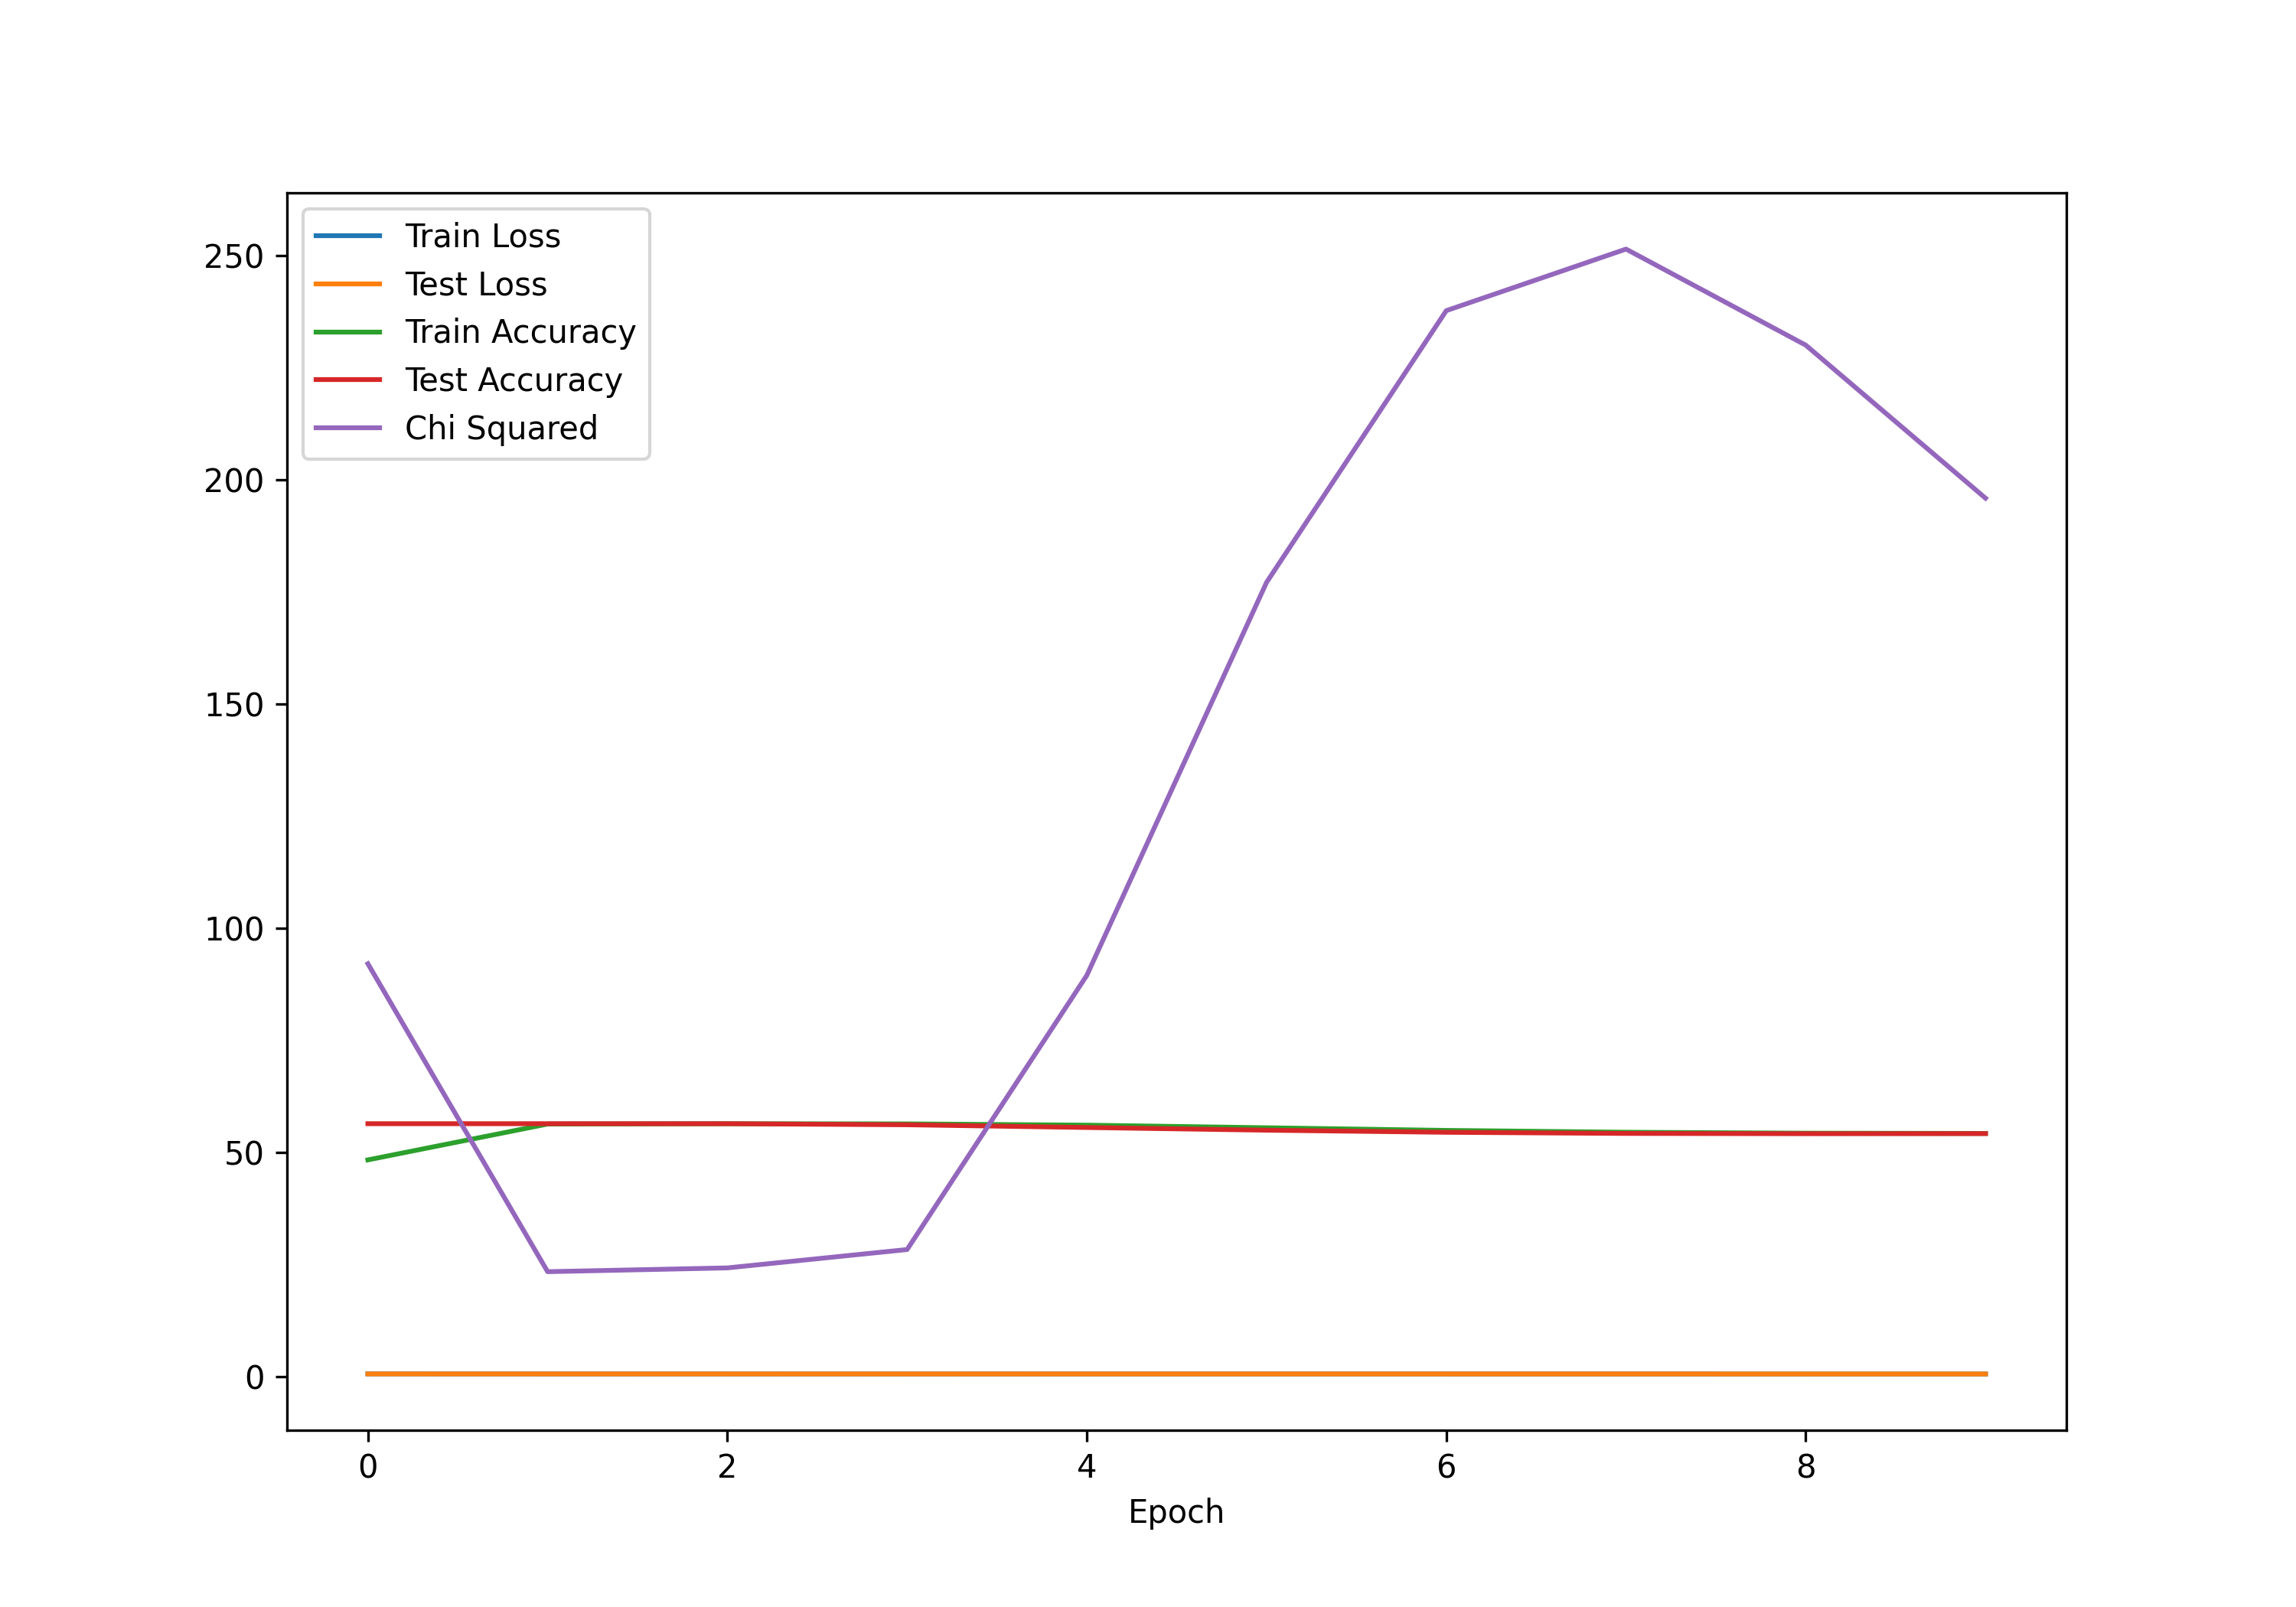
\includegraphics[width=\textwidth]{graphs/nn_incl_metrics.png}
        \caption{Shallow Model for Inclusive}
        \label{fig:accuracy_loss_incl}
    \end{subfigure}
    \hfill
    \begin{subfigure}[b]{0.45\textwidth}
        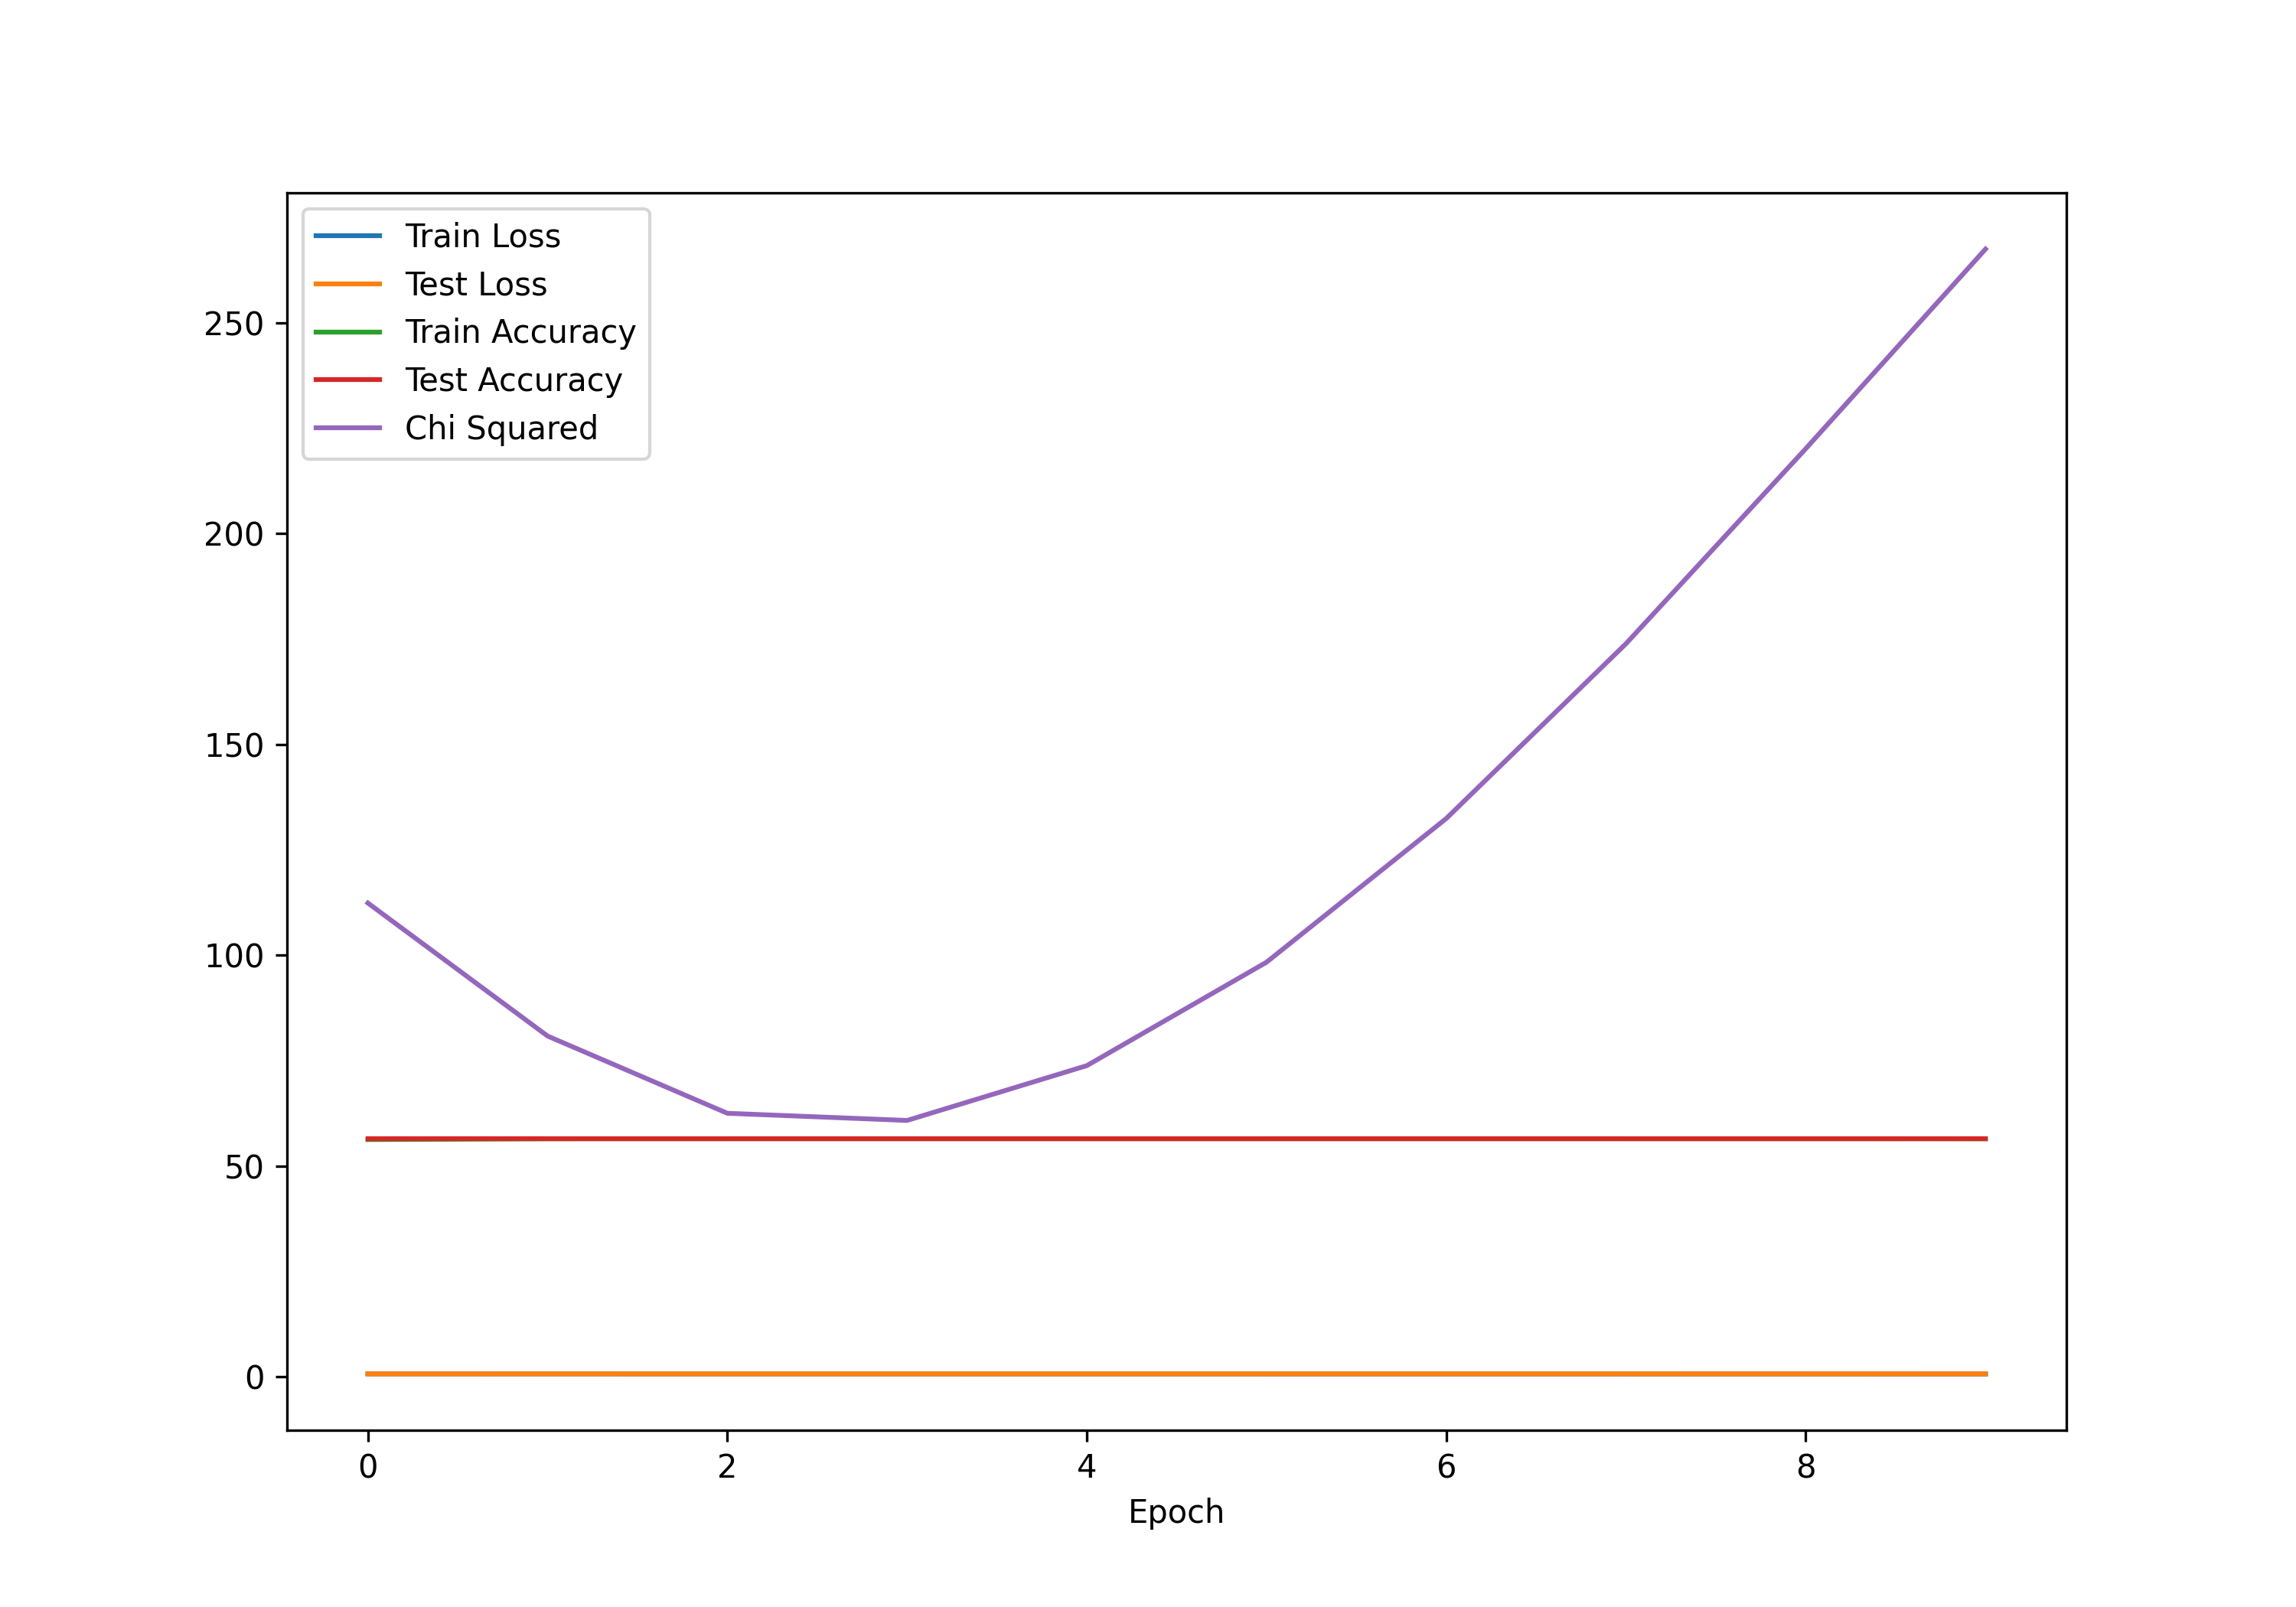
\includegraphics[width=\textwidth]{graphs/nn_incl_metrics_deeper.png}
        \caption{Deep Model for Inclusive}
        \label{fig:accuracy_loss_incl_deep}
    \end{subfigure}
    \caption{Comparison of Shallow and Deep Models for Inclusive}
\end{figure}



Please keep in mind that the image presented here represents just one of the training sessions.

As observed in the image above, the deeper model exhibited a relatively stable performance but yielded notably high chi-squared values. On the other hand, the less deep model displayed instability but delivered lower chi-squared values. Consequently, we made the decision to discontinue the deeper model and retain the less deep one.

Following multiple training sessions and employing a transfer learning approach—initiating the training process with the weights from the best-performing model among the previous runs—we successfully obtained models that met the required chi-squared criteria.

To evaluate the models, we calculated the mean value of the ratio of counts per bin between the data and the Neural Network output (one can also see this tensors simulating histograms in our code in the files with extenstion generalize.py). The results are presented in the table below:

\begin{table}[H]
    \centering
    \begin{tabular}{c|c}
    \textbf{Inclusive} & \textbf{Hadron} \\ \hline
    1.01702 & 1.28094 \\
    \end{tabular}
\end{table}


As evident from the above means, the model are making accurate predictions regarding the acceptance of COMPASS/AMBER.


\subsection{Genelarization with Other Data}
In order to assess the models' generalization capabilities, we employed a separate dataset and generated histograms for the Neural Network's output concerning both Inclusive and Hadron events.
We then proceeded to divide the output by the True Acceptance and calculated the mean value of the ratio, which is presented in the table below:

\begin{table}[H]
    \centering
    \begin{tabular}{c|c}
    \textbf{Inclusive} & \textbf{Hadron} \\ \hline
    1.00948 & 1.27528 \\ 
    \end{tabular}
\end{table}

As the ration is close to 1, one can say the models are predicting the acceptance of the COMPASS/AMBER as desired.

\section{Structure of the Spectometer}
Out of curiosity, we contemplated the possibility of utilizing the muon and hadron angles to attempt the reconstruction of the detector's structure. It is well understood that when particles interact with physical objects, they may either be absorbed or deflected, leading to a loss in acceptance. As a result, we proceeded to generate histograms for the angles of the muon and the hadron, the results of which can be observed in the figures below:

\begin{figure}[H]
    \centering
    \begin{subfigure}[b]{0.45\textwidth}
        \includegraphics[width=\textwidth]{graphs/incl_angle.png}
        \caption{Structure Reconstruction with Muon Angle}
        \label{fig:muon_angle}
    \end{subfigure}
    \hfill
    \begin{subfigure}[b]{0.45\textwidth}
        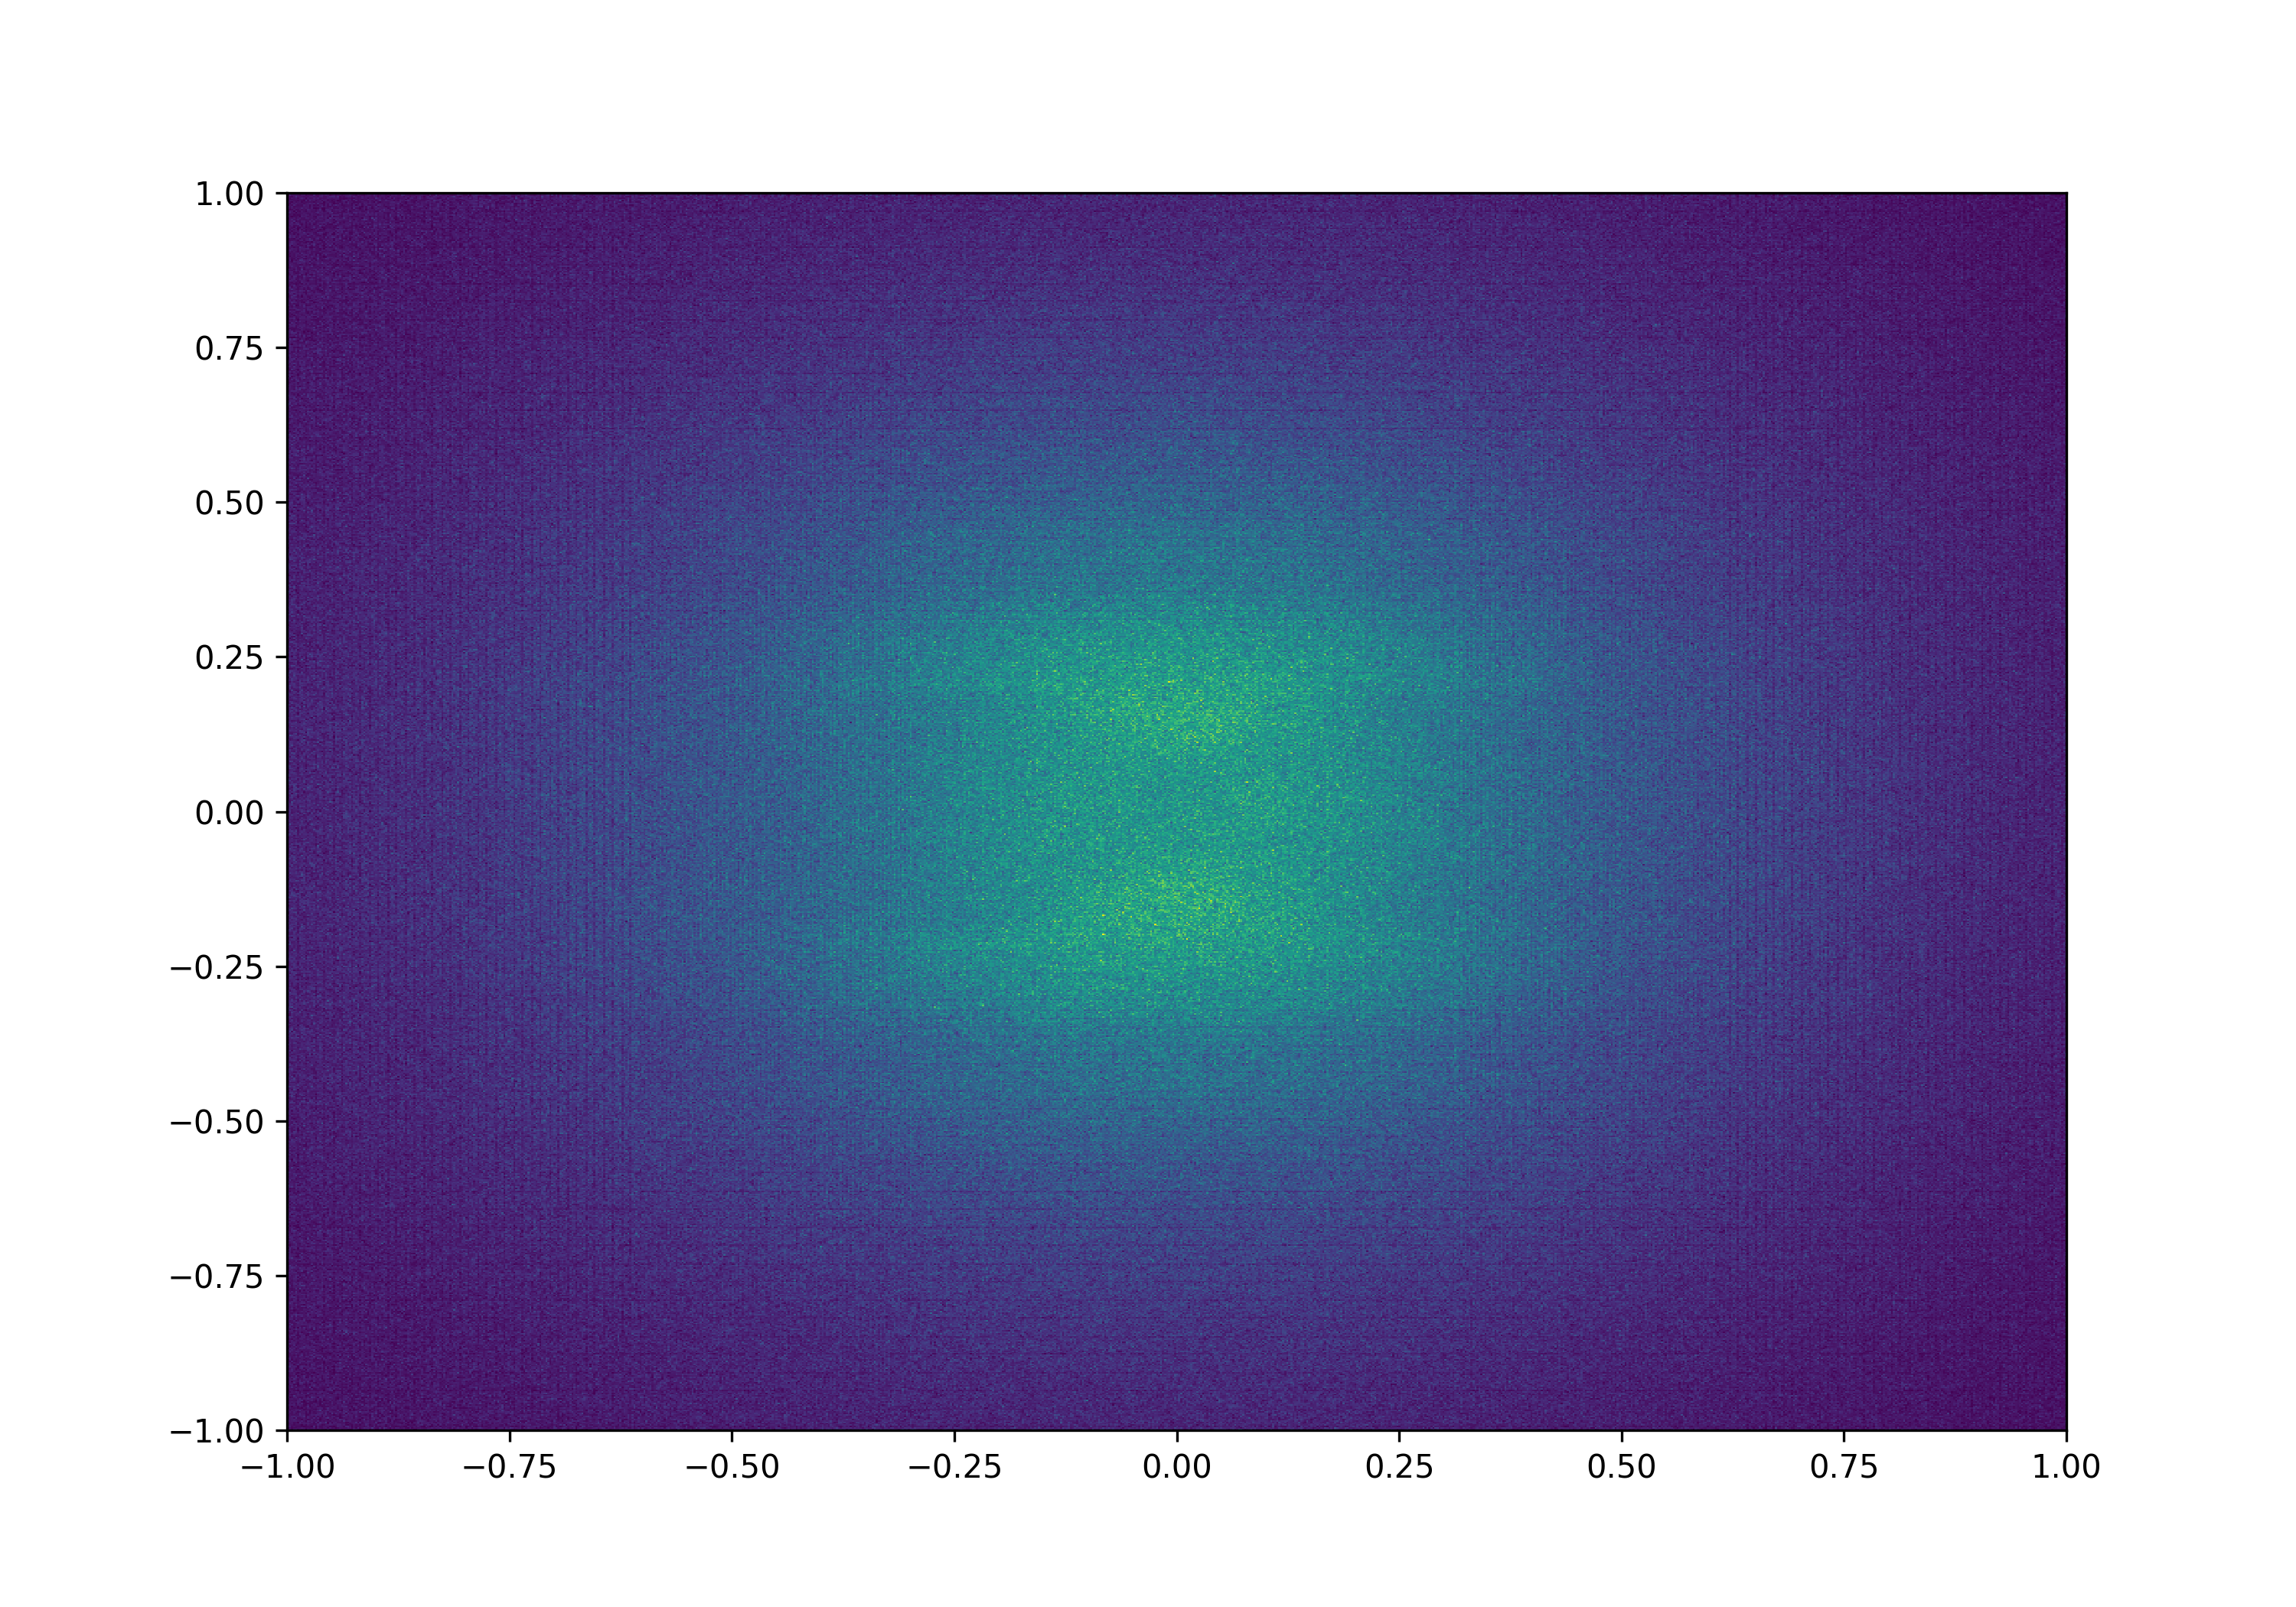
\includegraphics[width=\textwidth]{graphs/hadron_angle.png}
        \caption{Structure Reconstruction with Hadron Angle}
        \label{fig:hadron_angle}
    \end{subfigure}
    \caption{Structure Reconstruction with Muon and Hadron Angles}
\end{figure}

In the figure \ref{fig:hadron_angle} we can see a structure and a rectangular frame. To confirm if indeed it's
the structure of the spectometer, one need to have the real structure of the spectometer and compare it with the histogram.
Unfortunately, we don't have the real structure of the spectometer, so we cannot confirm if the histogram is indeed the structure of the spectometer.

In the figure \ref{fig:muon_angle} we can see kind of a hole in the middle of the histogram, which might indicate that all of the muons are going through the middle of the spectometer and not hitting the outer structure of the spectometer.



\section{Improvements}
This problem is inherently challenging due to the complex nature of the data and the substantial volume of events involved. As such, there is considerable potential for enhancement. One avenue for improvement involves exploring alternative Neural Network architectures, such as Convolutional Neural Networks (CNN), Recurrent Neural Networks (RNN), Graph Neural Networks (GNN), among others. It's worth noting that these architectures were not employed in this project due to constraints related to time, computational resources, and project scope.


\section{Conclusion}



\end{document}